\section{Simulation Results}

We can now test more complex setups by doing Bit Error Rate (BER) analysis.

\subsection{BER stocastic simulation}

\begin{figure}[H]
  \centering
  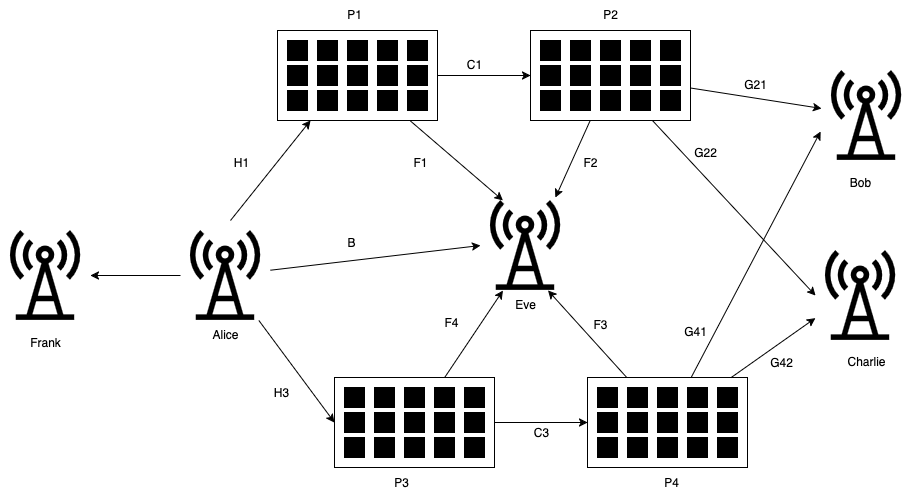
\includegraphics[width=\linewidth]{imgs/complex-situation.png}
  \caption{Complex Setup}
  \label{fig:correlation_sk2}
\end{figure}

For example, here we have a single transmitter \textit{Alice} and multiple receivers. \textit{Frank} is a direct receiver in line of sight. \textit{Bob} and \textit{Charlie} receive the signal from two double RIS reflection. \textit{Eve} receives both the direct signal and the reflecting signal from all RISs. \footnote{It should be noted that if \textit{Eve} is in the same position as \textit{Frank} and receives just the direct signal, our particular framework would not give us physical layer security, and higher layer security would be needed. If instead \textit{Eve} has not line of sight, the message would be completely unreadable from the start, since it would receive random matrixes.}

More in general, we would have $M$ consecutive RIS (in series) that reflect a signal, $J$ legitimate receivers and $Q$ different paths of RIS (in parallel) to send the signal at the same time. \footnote{The paths could have a different number of RIS (for example, a path of three and another of two). The results would still hold.}

We will show simulation results for different combinations of ($M, J$), both with a single and double path. In all scenarios, $K = 2, N = 16, \eta = 0.9$ will be the number of antennas for all actors, the number of reflecting surfaces and the reflection coefficients. We take these parameters to compare the results to the original paper \cite{9328149}.

The direct link and the eavesdropper will try to understand the message by following the equation \eqref{eq:direct_detection}, while the receivers will try to understand it by following the equation \eqref{eq:reflection_detection}.

\subsubsection{Single RIS reflection (M=1)}

\begin{figure}[H]
  \centering
  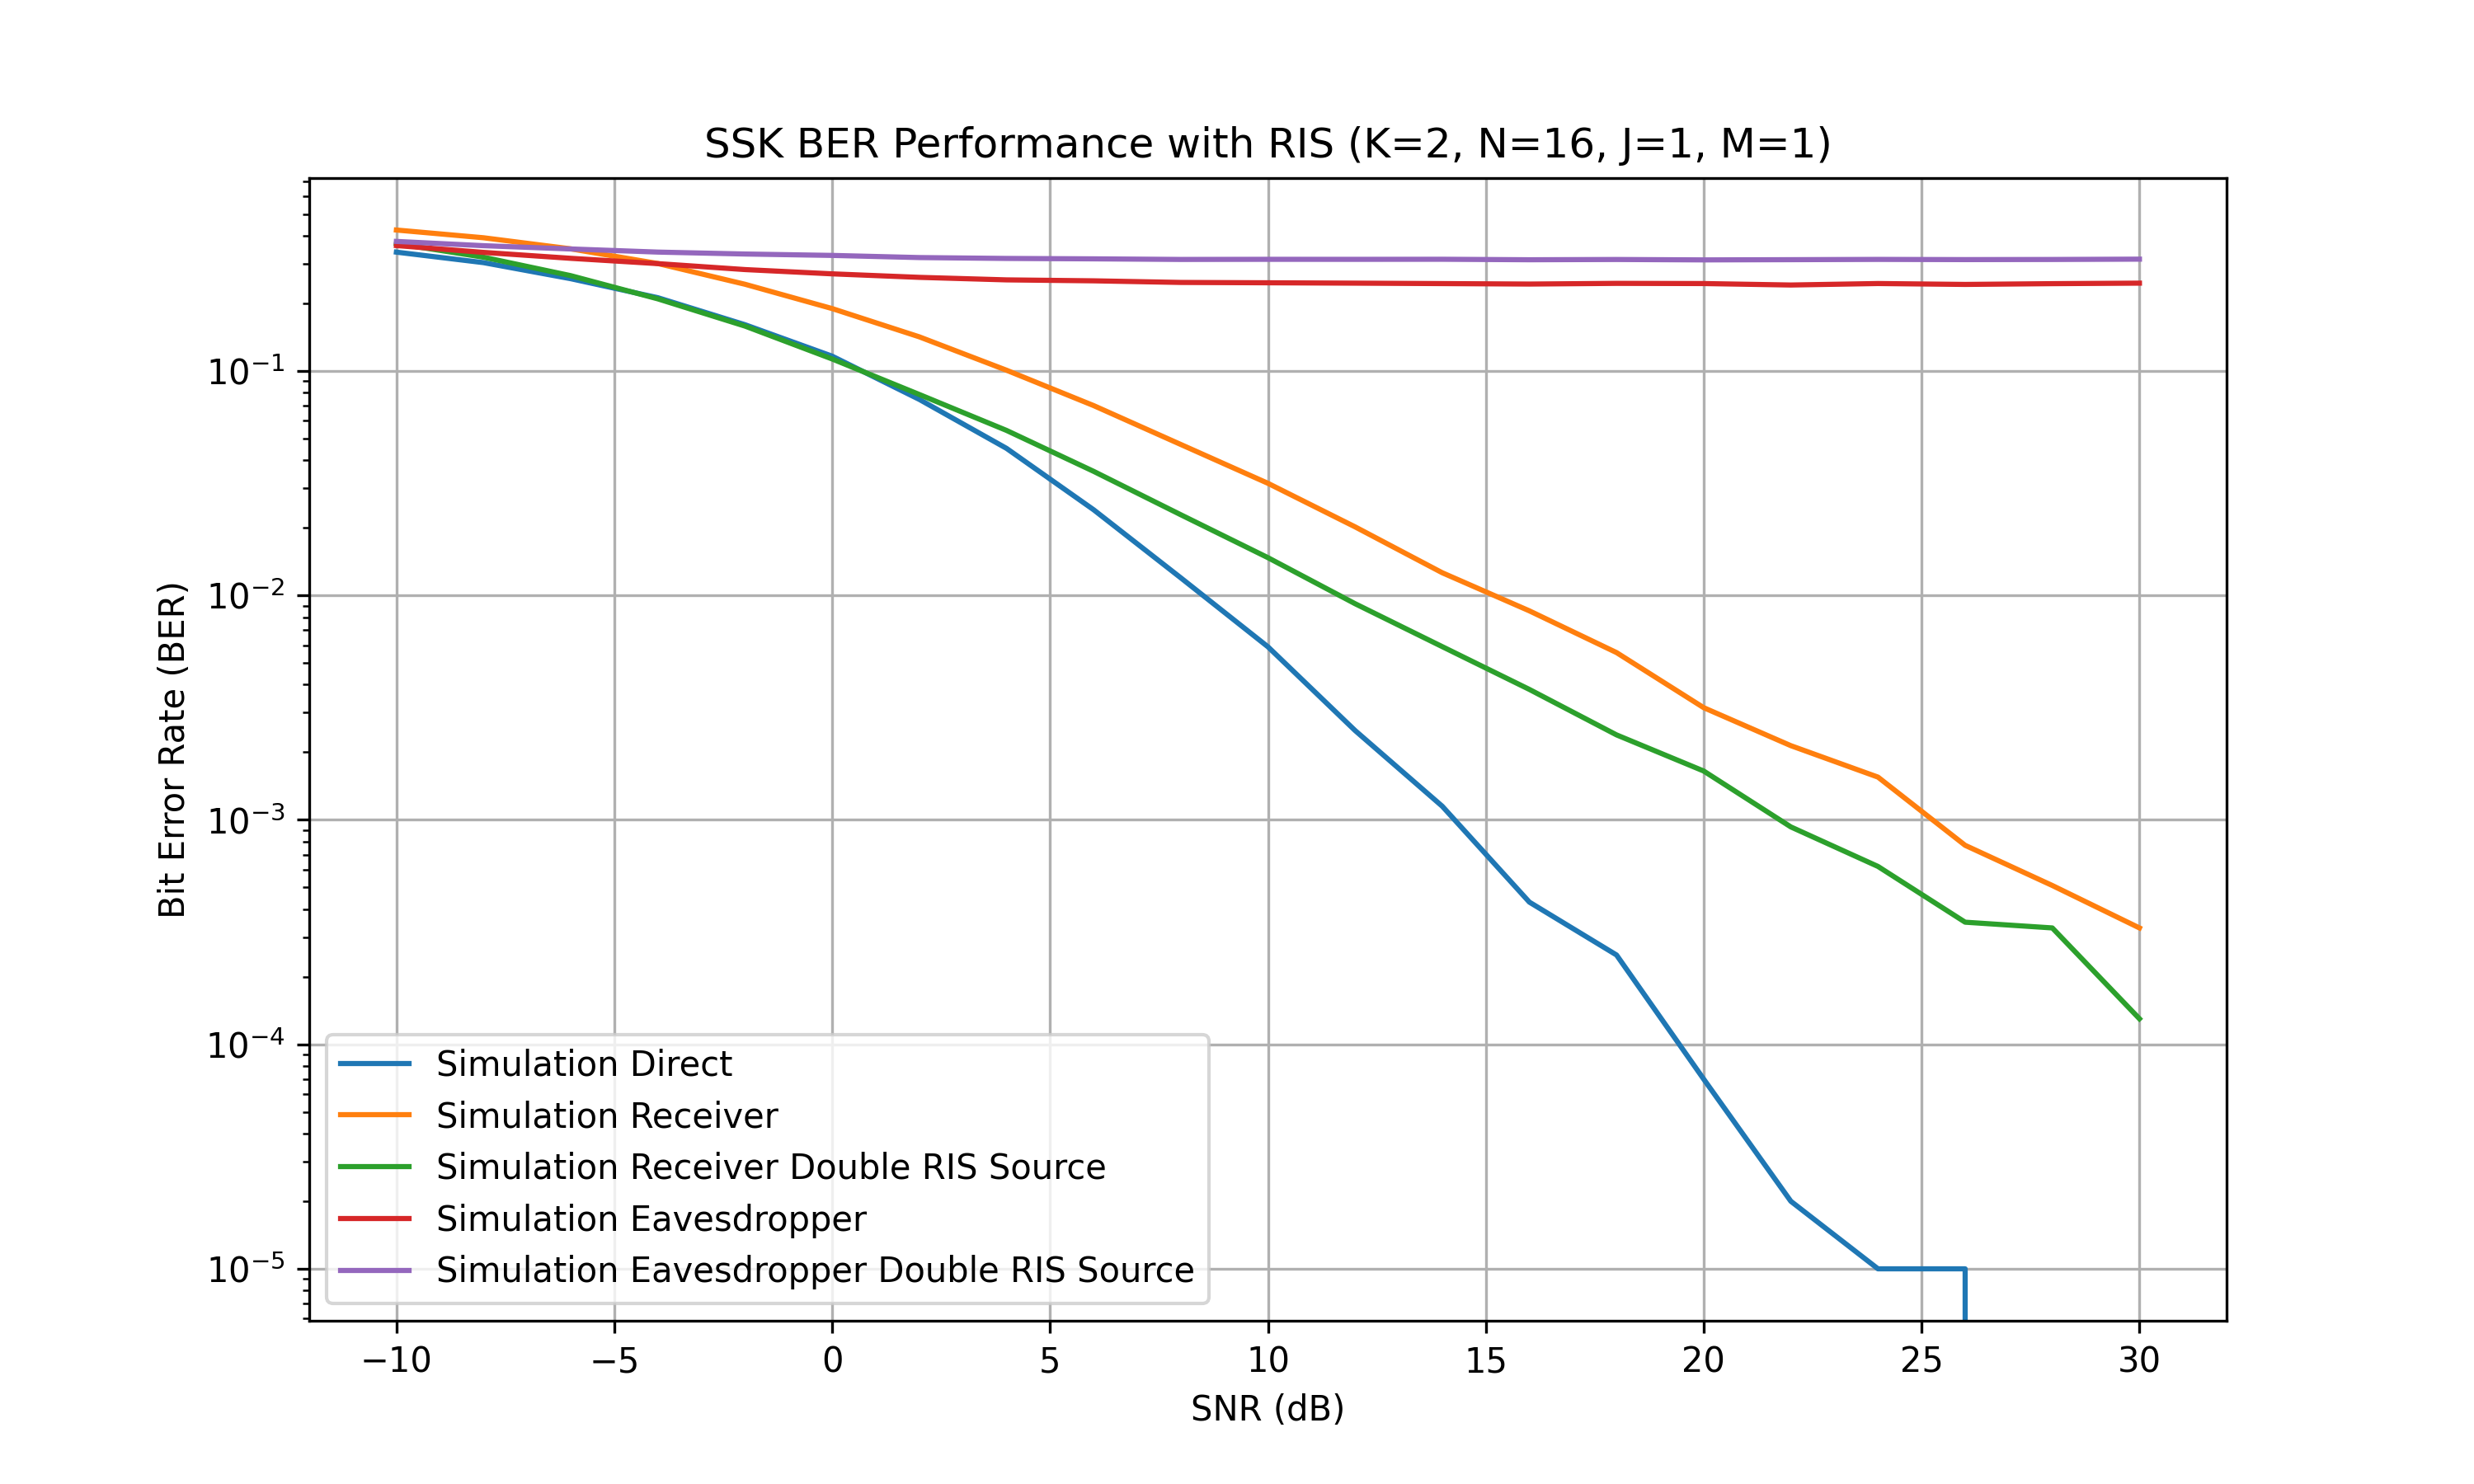
\includegraphics[width=0.9\linewidth]{imgs/ber-simulations/SSK BER Performance with RIS (K=2, N=16, J=1, M=1).png}
  \caption{SSK BER Performance with RIS (K=2, N=16, J=1, M=1)}
  \label{fig:simulation_j1_m1}
\end{figure}

We can see in ($M=1, J=1$) the results match with \cite{9328149}, for both \textit{Simulation Receiver} and \textit{Simulation Eavesdropper}.
\textit{Simulation Direct} is the strongest possible path, mainly because of the reflection loss due to $\eta$.
Combining two different RIS in parallel (\textit{Double RIS Source}) gives better signal to the receiver, while disturbing more the signal to the eavesdropper.

\begin{figure}[H]
  \centering
  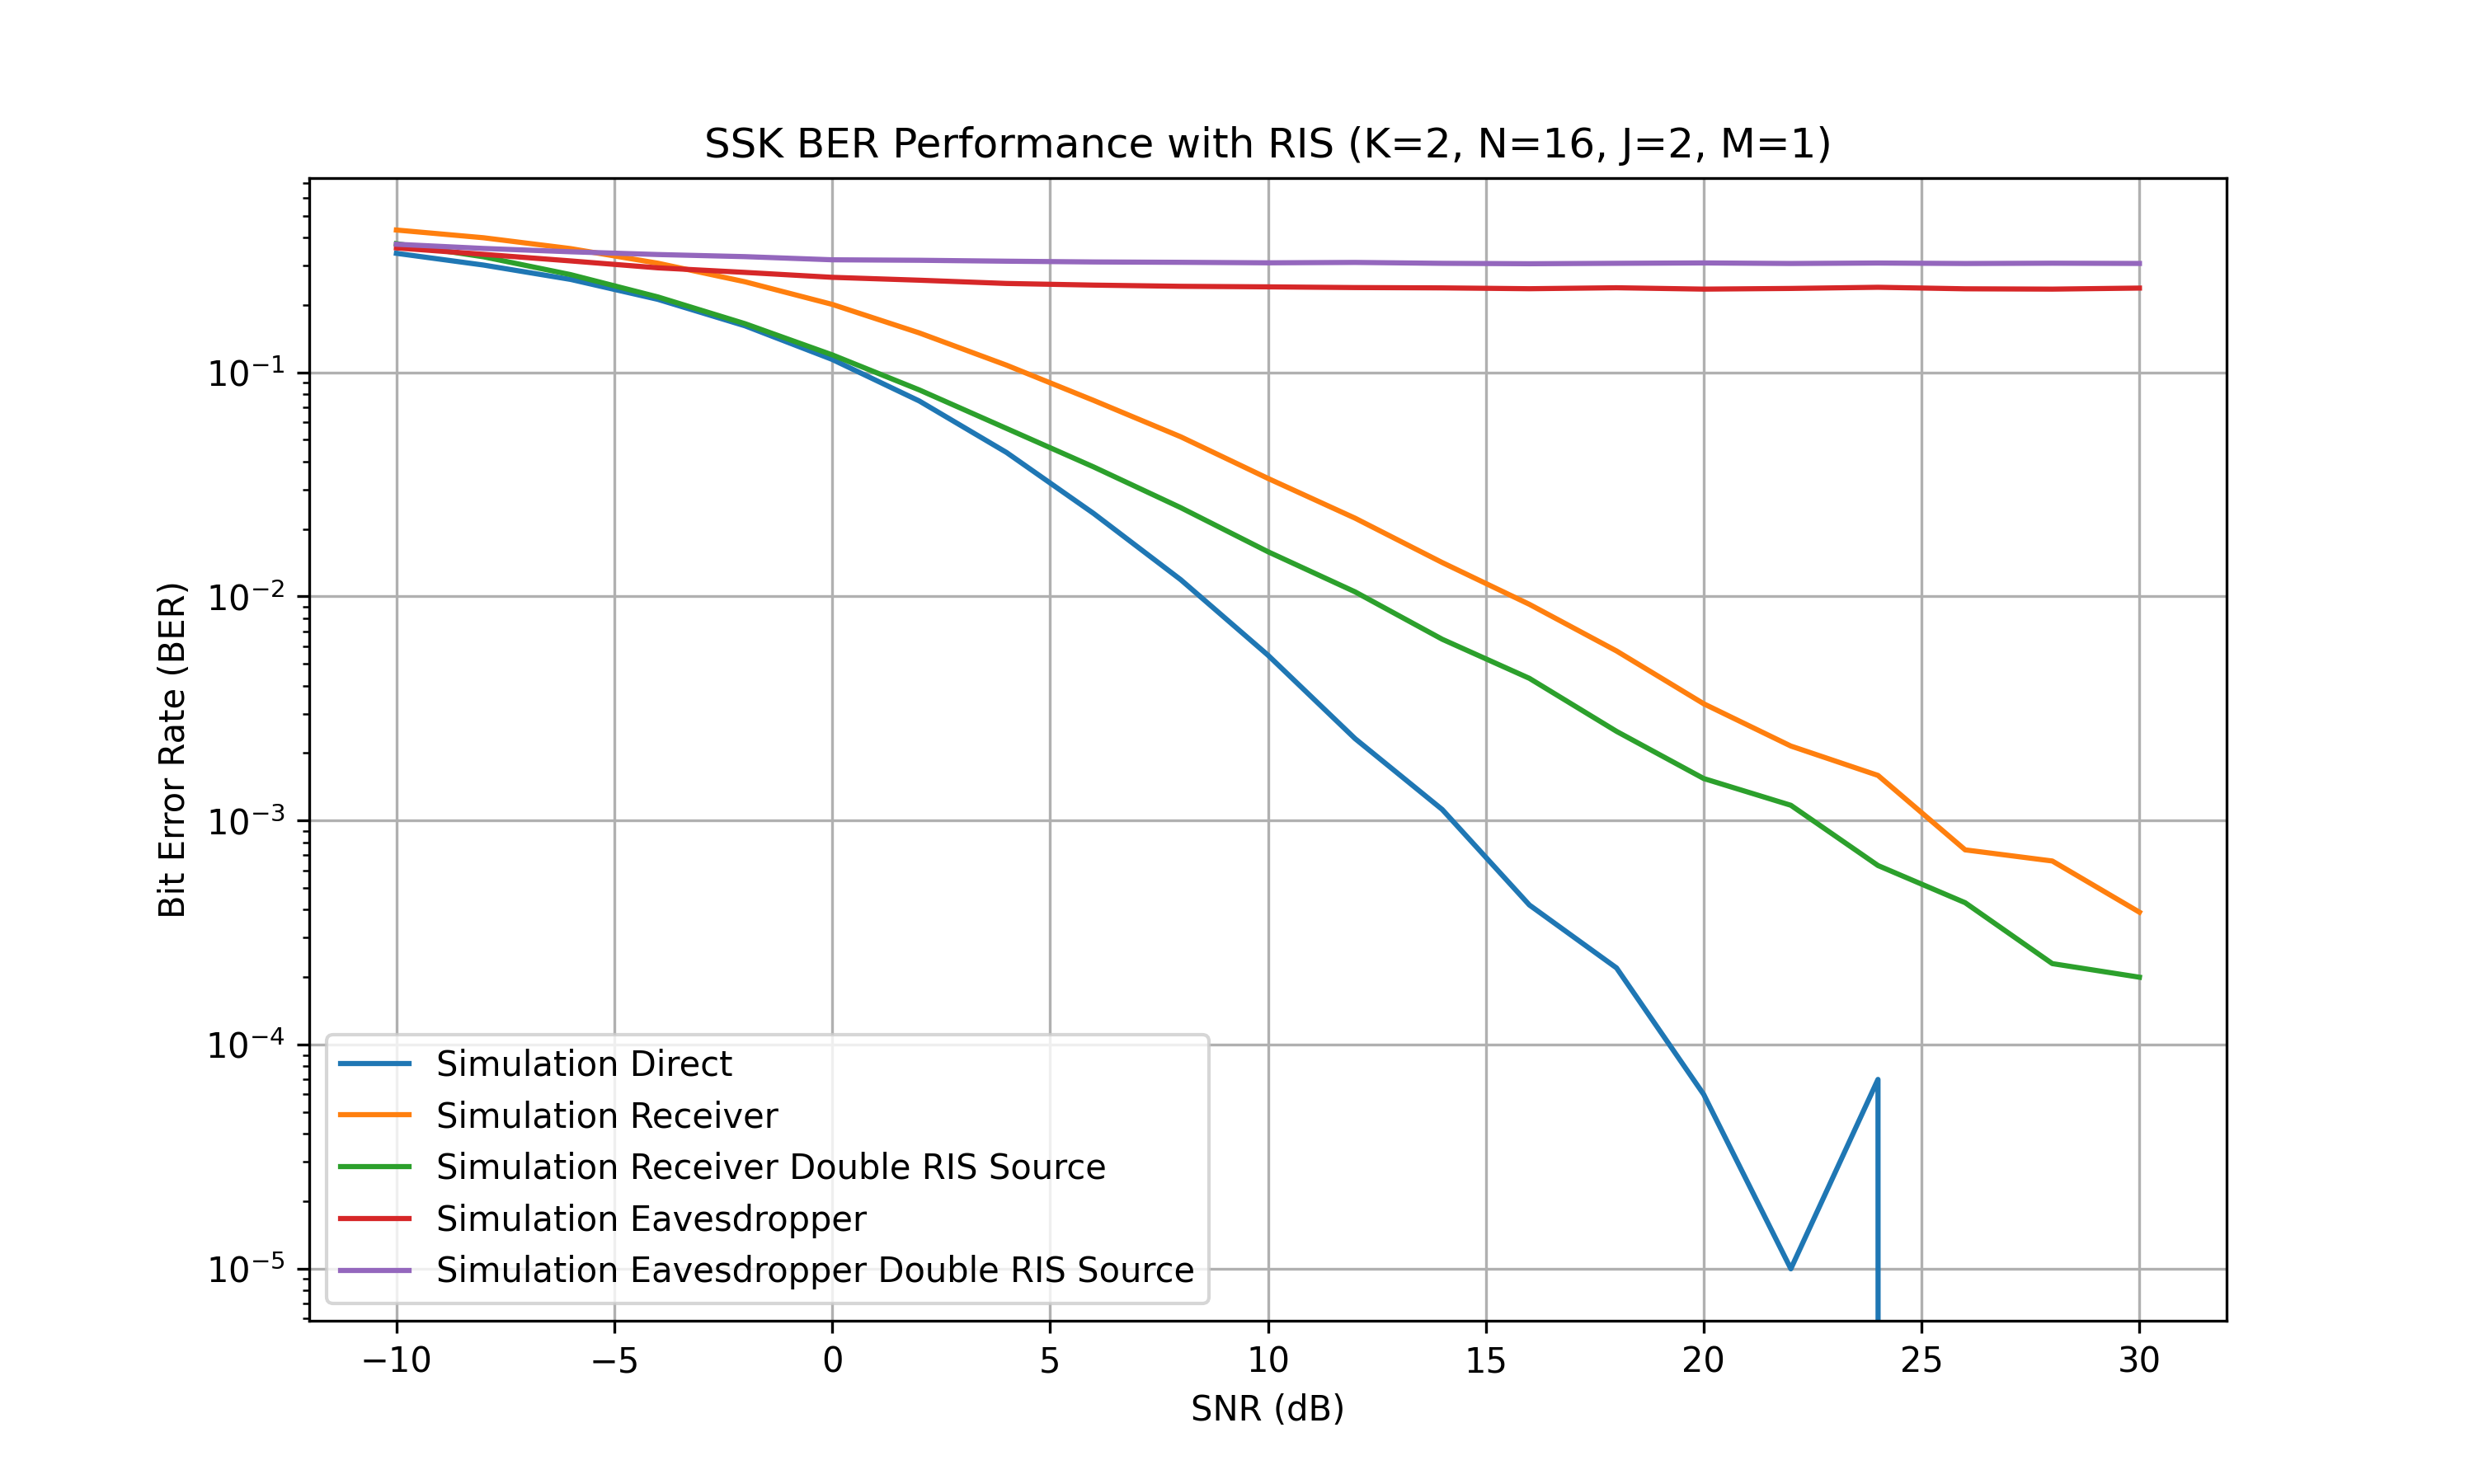
\includegraphics[width=0.9\linewidth]{imgs/ber-simulations/SSK BER Performance with RIS (K=2, N=16, J=2, M=1).png}
  \caption{SSK BER Performance with RIS (K=2, N=16, J=2, M=1)}
  \label{fig:simulation_j2_m1}
\end{figure}

Increasing the number of receivers does not influence the result of our framework: the receivers still get a good signal depending on the SNR, while the eavesdropper is not getting an advantage in understanding the message.

\subsubsection{Double RIS reflection (M=2)}

\begin{figure}[H]
  \centering
  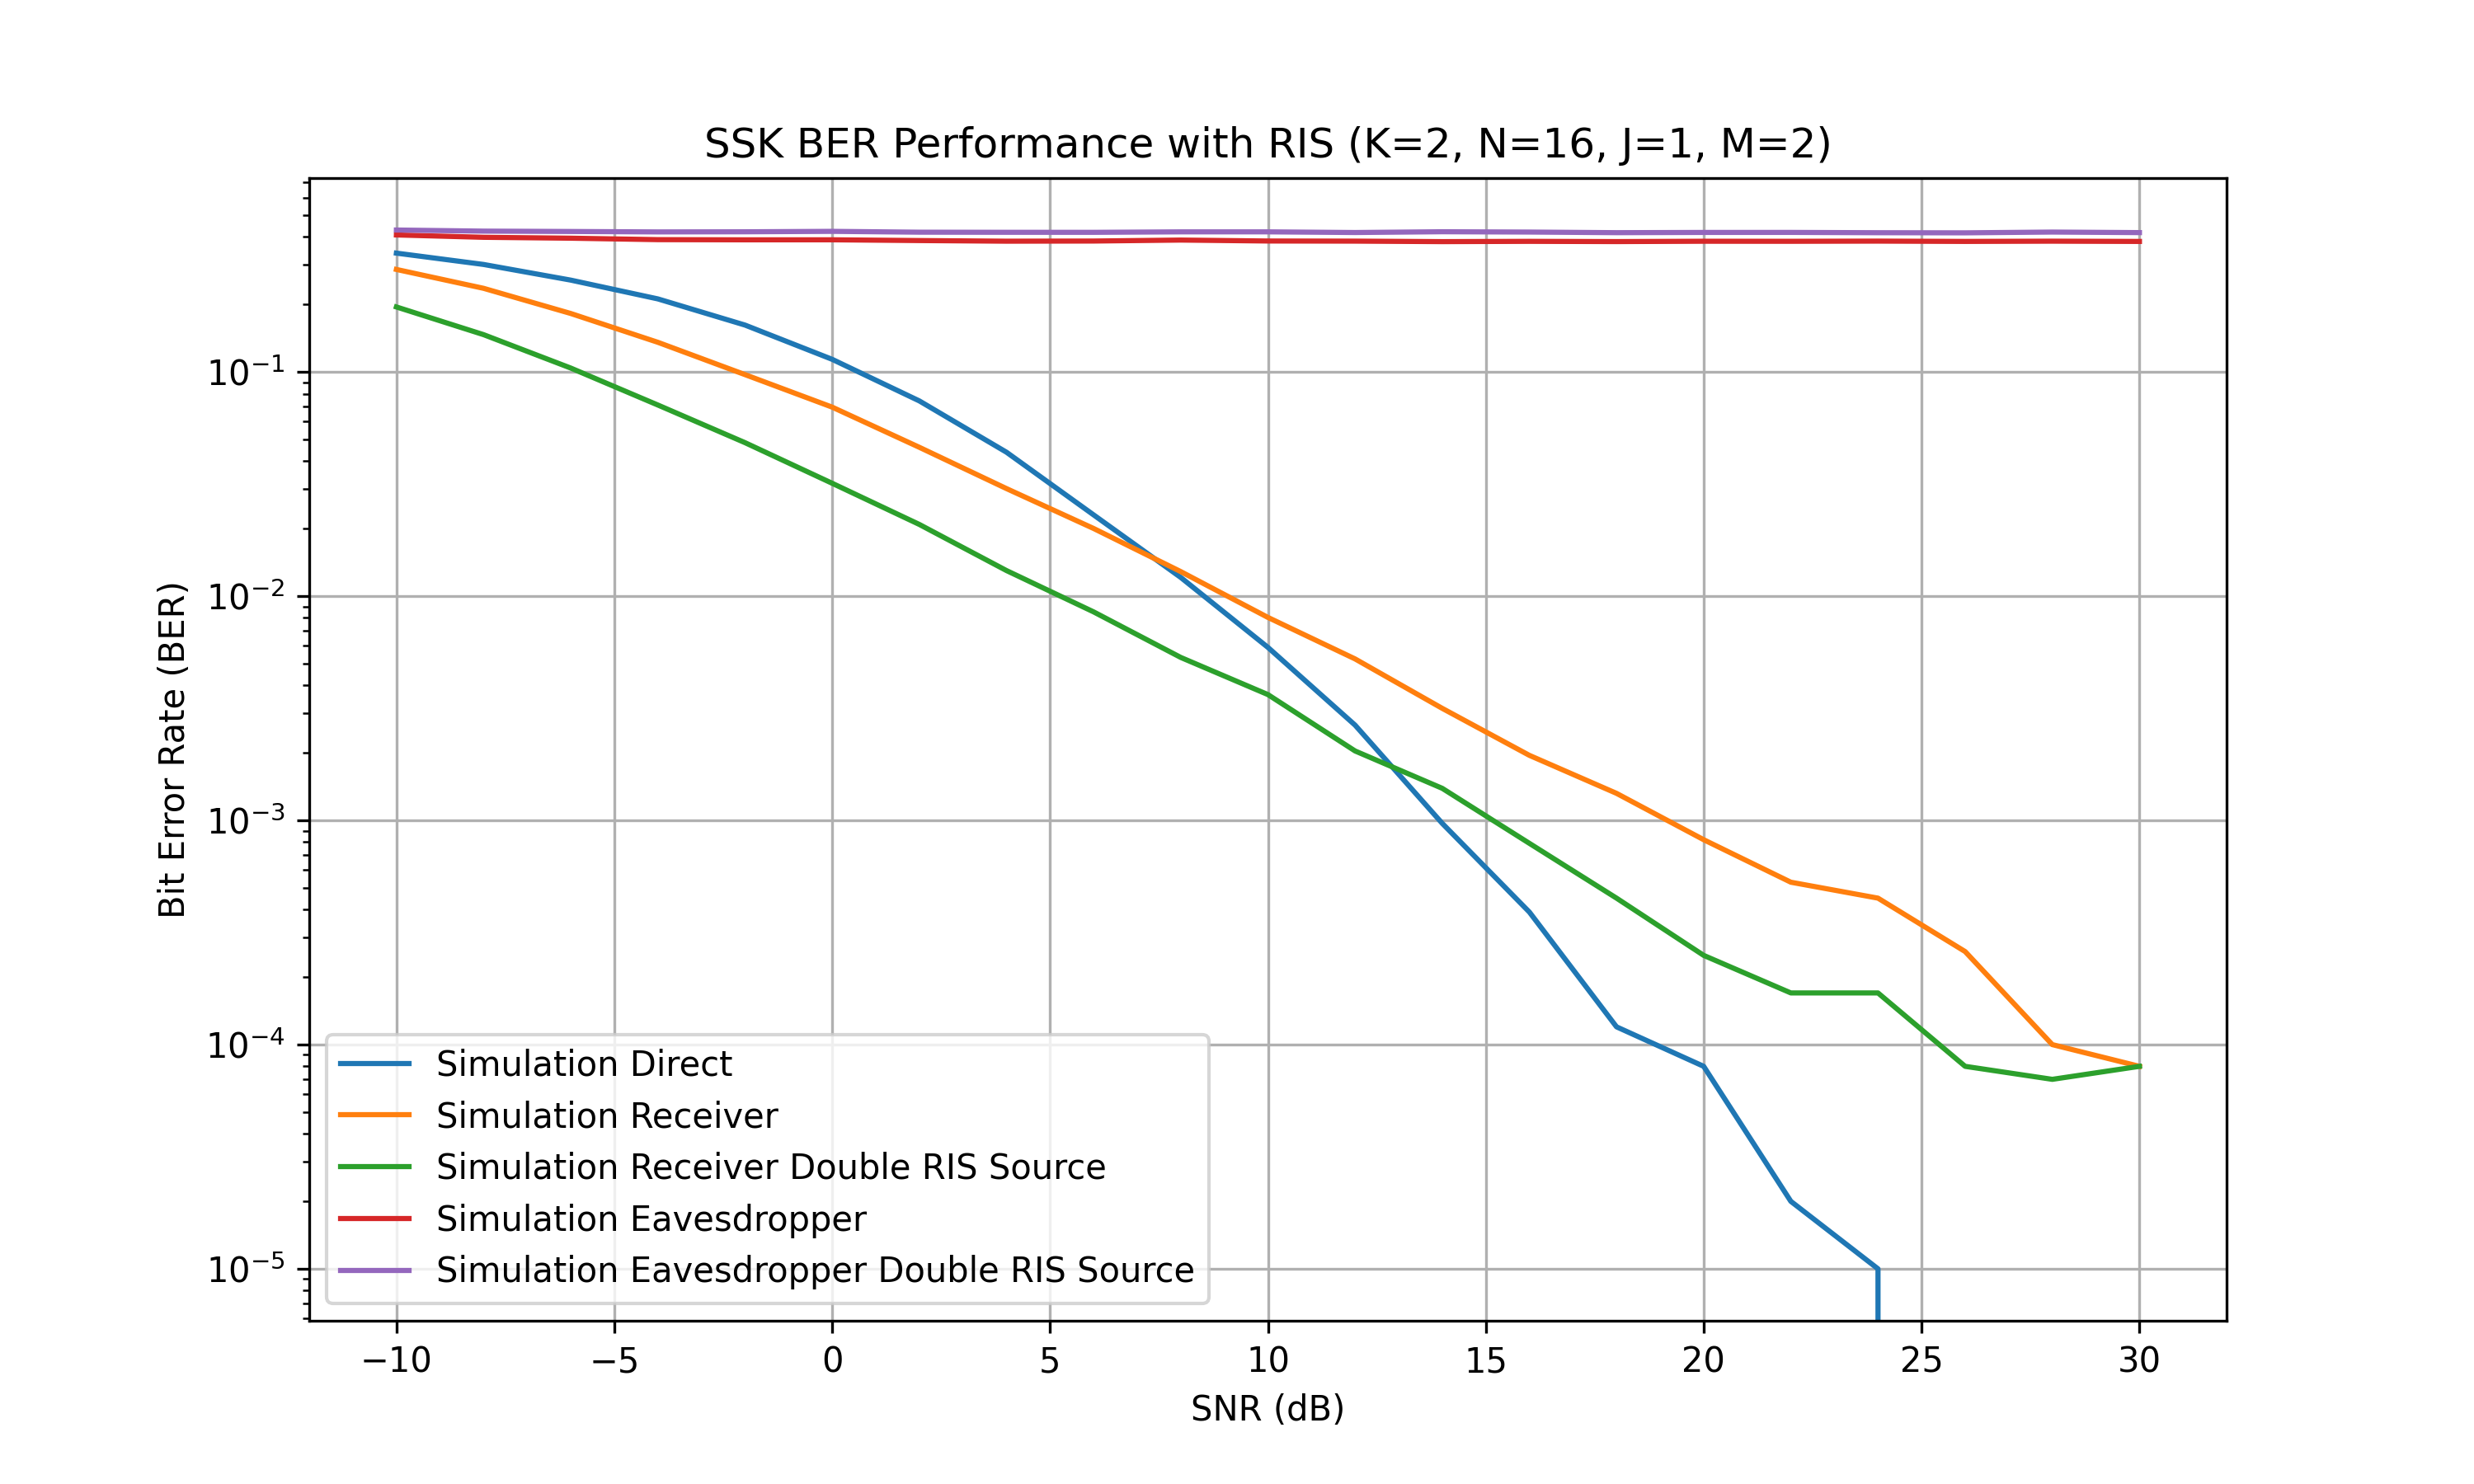
\includegraphics[width=0.9\linewidth]{imgs/ber-simulations/SSK BER Performance with RIS (K=2, N=16, J=1, M=2).png}
  \caption{SSK BER Performance with RIS (K=2, N=16, J=1, M=2)}
  \label{fig:simulation_j1_m2}
\end{figure}

With multiple RIS in series, the eavesdropper get a worse signal because of the double interference of the 2 RIS.
% \textbf{(TODO: Why the receiver is getting a better signal? Should it not be worse? Check normalization of the signal)}

\begin{figure}[H]
  \centering
  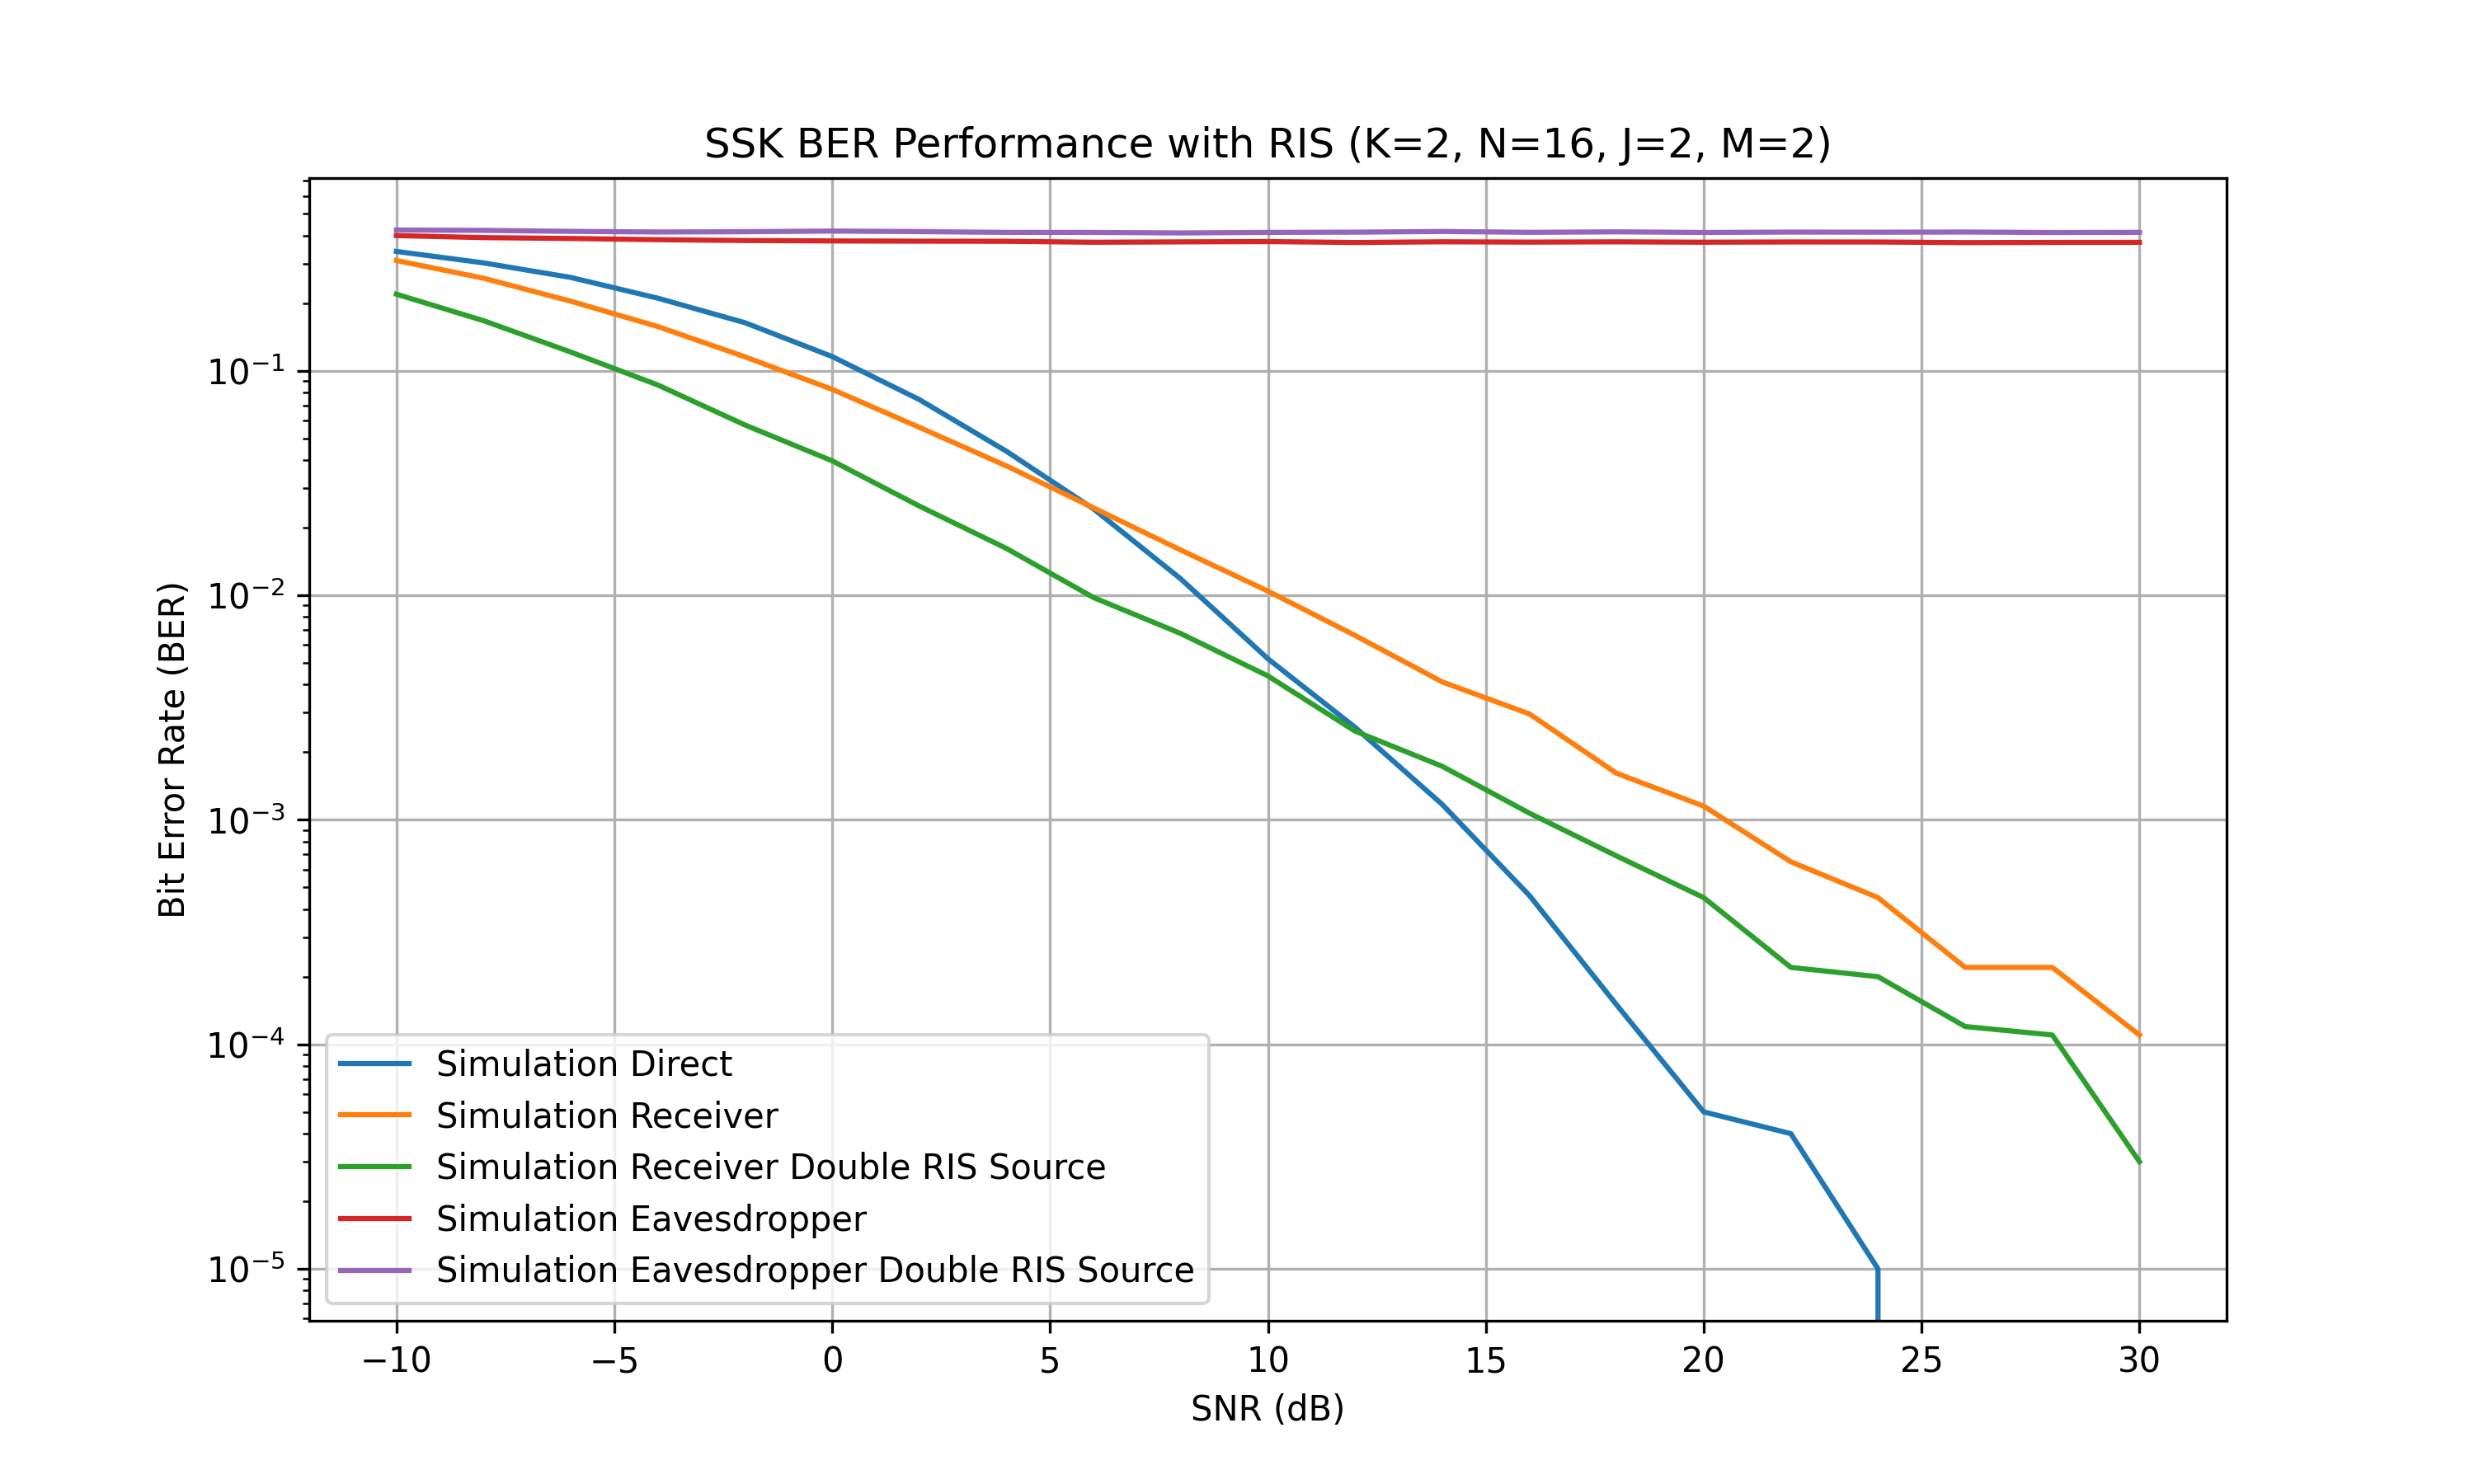
\includegraphics[width=0.9\linewidth]{imgs/ber-simulations/SSK BER Performance with RIS (K=2, N=16, J=2, M=2).png}
  \caption{SSK BER Performance with RIS (K=2, N=16, J=2, M=2)}
  \label{fig:simulation_j2_m2}
\end{figure}

Combining all together, our properties still hold strong.

\newpage
\subsection{BER realistic scenario simulation}

We can now simulate our framework in a realistic scenario. We first need to model the channel gain $H$ and the path loss, based on the distance between the actors. We will define $\lambda$ as the wavelenght of the signal, and $d$ as the distance between two actors.

\subsubsection{Channel gain calculation}

We model the Rician fading \cite{Rician_fading} matrix $\bm{\Xi}$, to consider possible fading due to multipath interference. Using the Shape Parameter $\tau$, defined as the ratio of the power contributions by line-of-sight path to the remaining multipaths, and the Scale parameter $\xi$, defined as the total power received in all paths, we can calculate

\begin{equation}
  \nu^2 = \frac{\tau \xi}{1 + \tau}
\end{equation}
\begin{equation}
  \sigma^2 = \frac{\xi}{2(1 + \tau)}
\end{equation}

and we can generate $\bm{\Xi}$ by creating a random complex matrix where the real and the imaginary values are extracted from a gaussian distribution $C(\frac{\nu}{\sqrt{2}}, \sigma)$ \cite{Rice_distribution}

Then, given an actor $r$ with $n_r$ antennas disposed as a \textit{uniform linear array}, we can define the \textit{unit spatial signature in the directonal cosine $\Omega = cos \phi$} \cite{Fundamentals_Wireless_Communication_chapter7} as

\begin{equation}
  e_r(\Omega) = \frac{1}{\sqrt{n_r}}
  \begin{bmatrix}
    1                                \\
    exp(-j2\pi\Delta\Omega)          \\
    exp(-j2\pi2\Delta\Omega)         \\
    \vdots                           \\
    exp(-j2\pi(n_r - 1)\Delta\Omega) \\
  \end{bmatrix}
\end{equation}

where
\begin{itemize}
  \item $\Delta$ is the distance between the antennas (usually $\lambda / 2$)
  \item $\phi$ is the angle of incidence of the line-of-sight onto the actor antenna
\end{itemize}

and we can model the channel gain matrix \cite{Fundamentals_Wireless_Communication_chapter7} as

\begin{equation}
  \bm{H} = \bm{\Xi} \odot \sqrt{n_t n_r} exp(-j2 \pi d / \lambda) e_r(\Omega_r) e_t(\Omega_t)^H
\end{equation}

This equation can be used both for a direct transmission between two actors, or between an actor and a RIS.

\subsubsection{Path loss calculation}

We begin by modeling the free space path loss \cite{Free_space_path_loss} between two points as
\begin{equation}
  \bm{PL} = ((4 \pi / \lambda)^2 d^k)^{-\frac{1}{2}}
\end{equation}
where $k$ is equal to $2$ when the antennas are isontropic % \textbf{(TODO explanation)}

For a direct LOS communication between the transmitter and another actor (either a legitimate receiver or an eavesdropper), the signal received from input $x$ would be

\begin{equation}
  y = \bm{PL}_B * \bm{B}x
\end{equation}

Given a reflected signal with channel gain $GPH$, where
\begin{itemize}
  \item $\bm{G}$ is the communication transmitter-RIS
  \item $\bm{H}$ is the communication RIS-actors
  \item $\bm{P}$ is the RIS reflection coefficient diagonal matrix
\end{itemize}
we have two different LOS communications. We have different way of calculating the total path loss:
\begin{itemize}
  \item we consider the RISs to be active, meaning they amplify the signal received before reflecting it and so they negate the path loss reduction. The signal received would be $y = PL_H * GPHx$. In case of multiple RISs, only the last connection path loss is considered. We will call this as a \textit{active path loss}
  \item we consider two separate path losses, one for each LOS. The signal received would be $y = PL_G * PL_H * \bm{GPH}x$. In case of multiple RISs, we multiply the path loss of all connections. We will call this as a \textit{product path loss}
  \item we consider one single path loss from the sum of the two distances ($d = d_{t-RIS} + d_{RIS-r}$). The signal received would be $y = PL_{G+H} * \bm{GPH}x$. In case of multiple RISs, we add all the distances. We will call this as a \textit{sum path loss}
\end{itemize}

We will see how these different considerations vary the results and the efficacy of the proposed framework.
\begin{itemize}
  \item with \textit{active path loss}, the RIS channel power is of the same order of magnitude as the transmitter channel power, so the direct signal receives significant noise
  \item with \textit{product path loss}, the RIS channel power is orders of magnitude smaller. The message remains hidden in areas without direct line of sight to the transmitter
  \item with \textit{sum path loss}, the disturbance effect is still visible, although less effective. It also the one with the results most similar to the theoretical simulation we made in the previous section.
\end{itemize}

The graphs below show some example situations, and prove our framework does also work in more realistic situations. Below, we used $\lambda = 0.08m, \tau = 0.6, \xi = 1, \eta = 0.9, SNR = 10db, K = 2, N = 16$. Each square represent an actor receiveing the signal (an eavesdropper, or a legitimate receiver if shown), with its own BER.

% \newpage

% \begin{figure}[H]
%   \centering
%   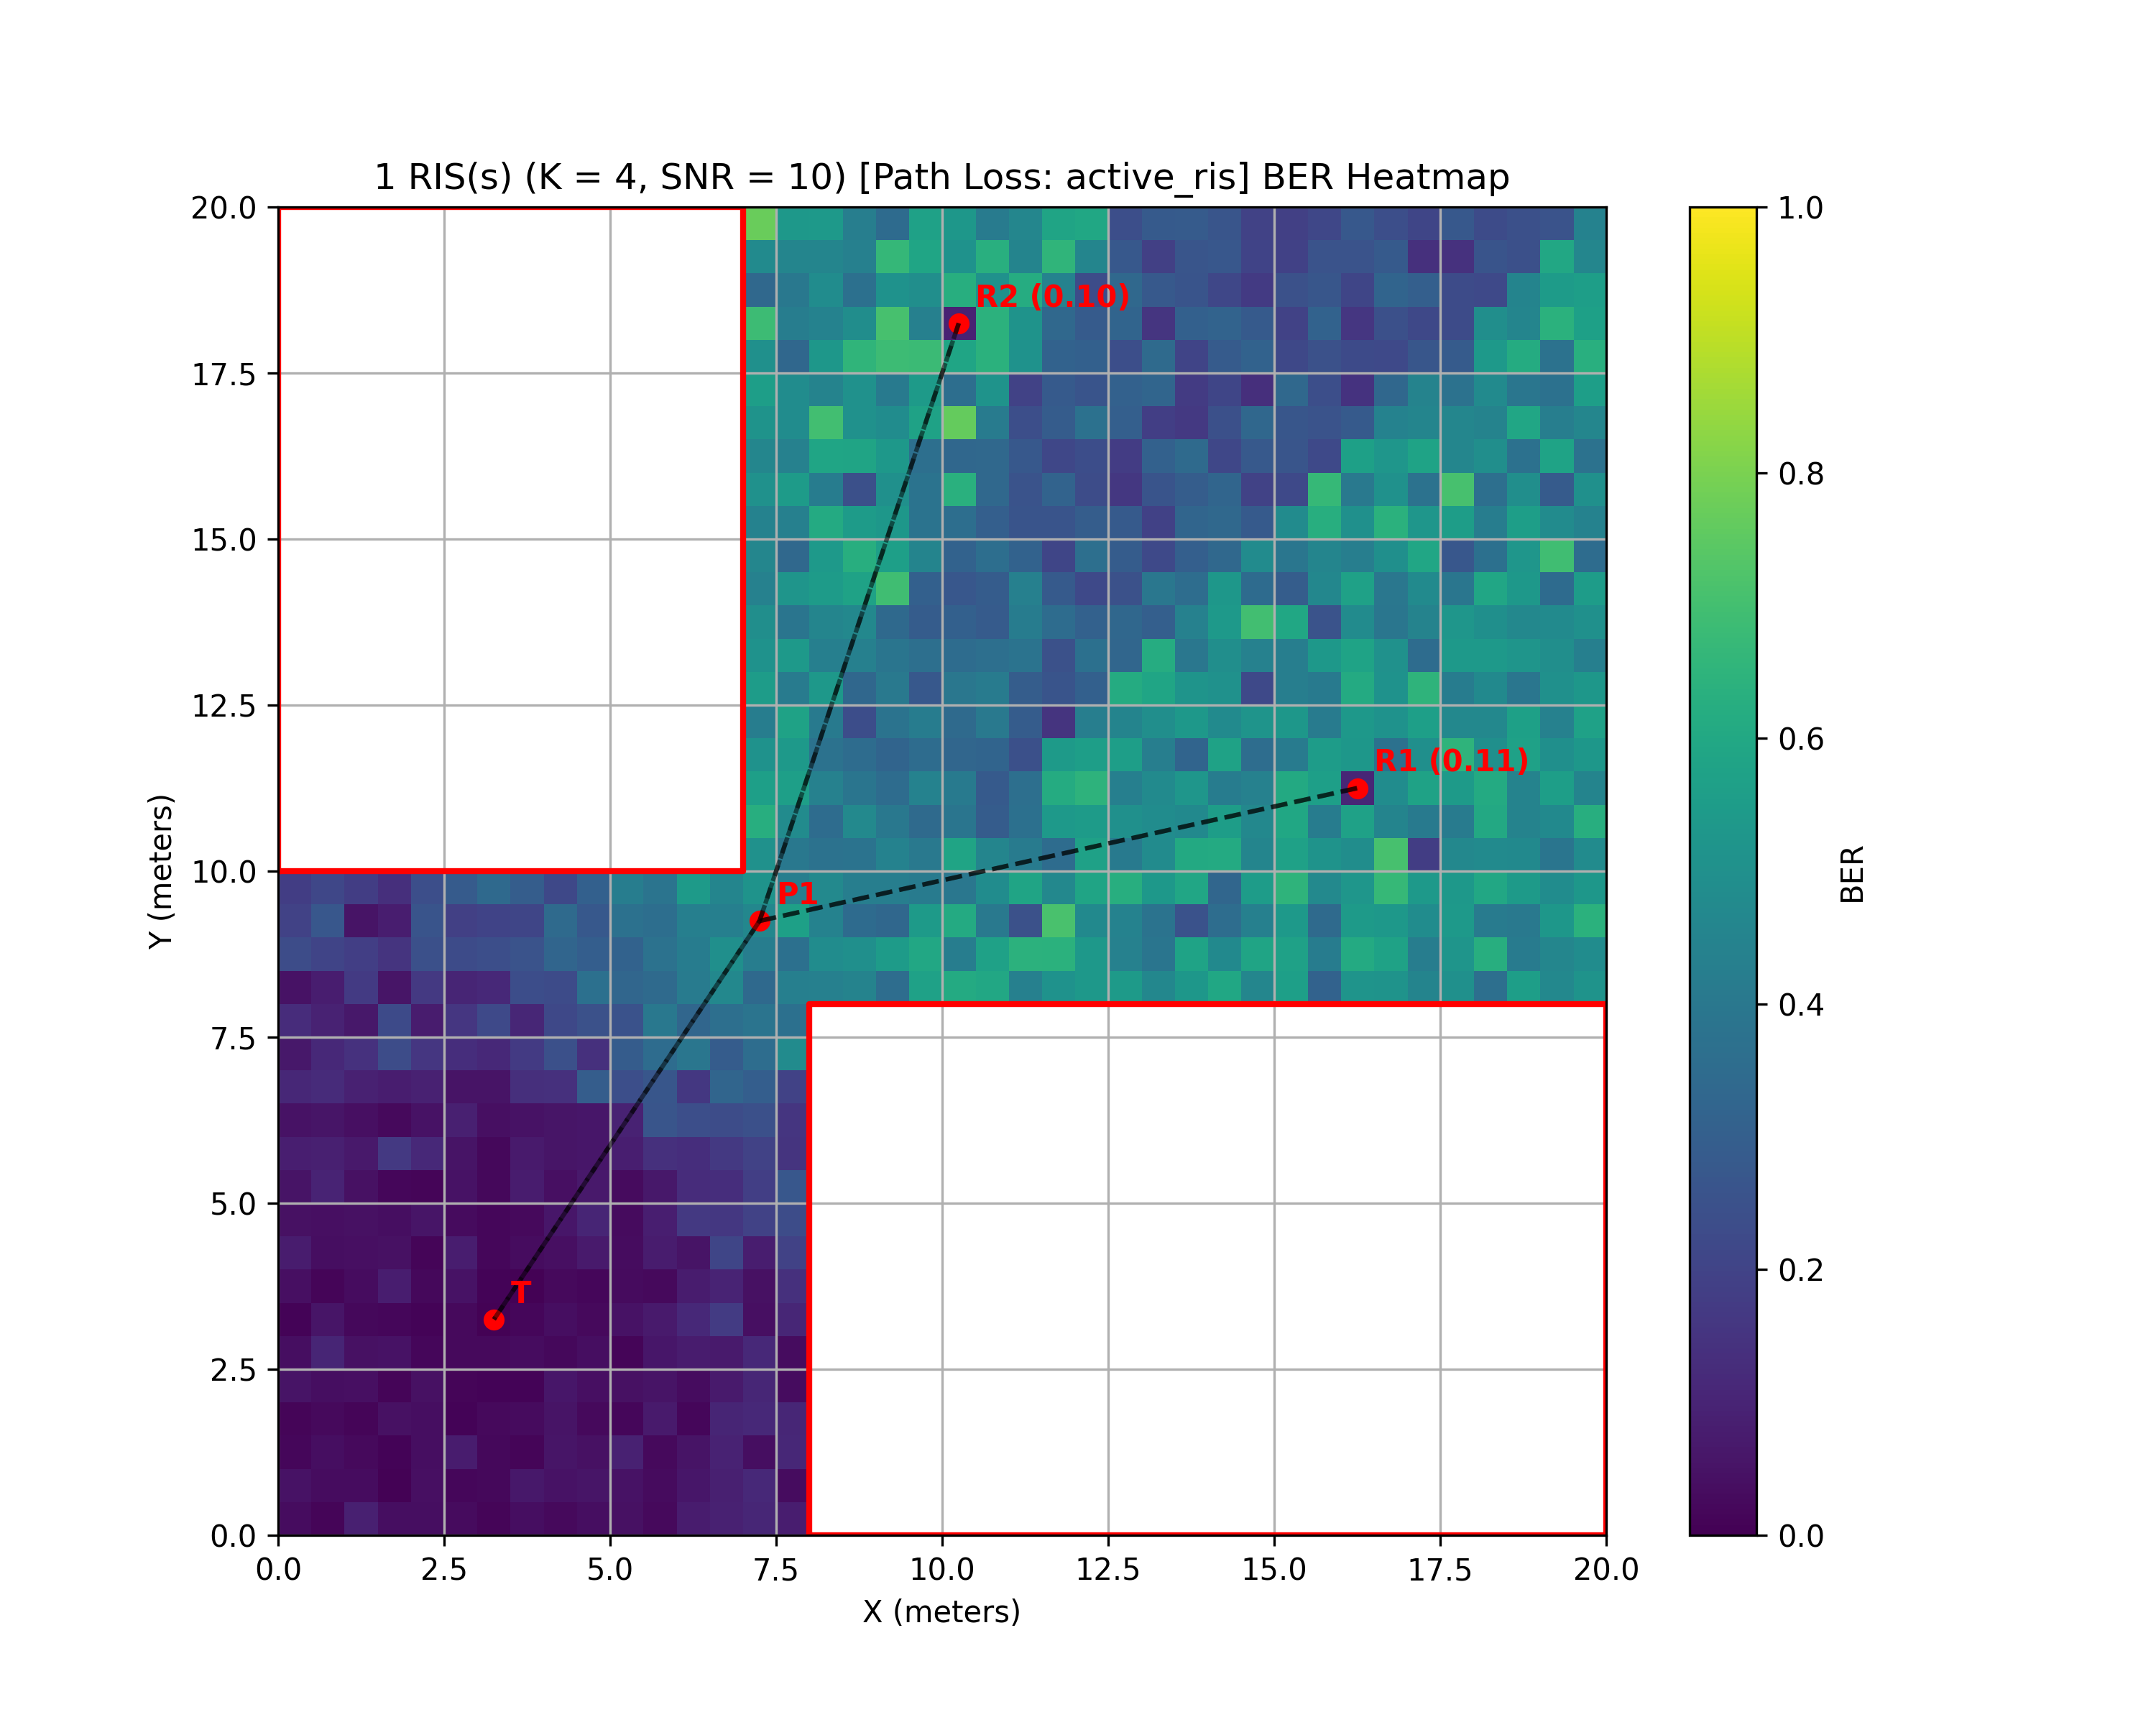
\includegraphics[width=0.8\linewidth]{imgs/heatmap-simulations/1 RIS(s) (K = 4, SNR = 10) [Path Loss_ active_ris] BER Heatmap.png}
%   \caption{1 RIS(s) (K = 4, SNR = 10) [Path Loss: active ris] BER Heatmap}
% \end{figure}

% \begin{figure}[H]
%   \centering
%   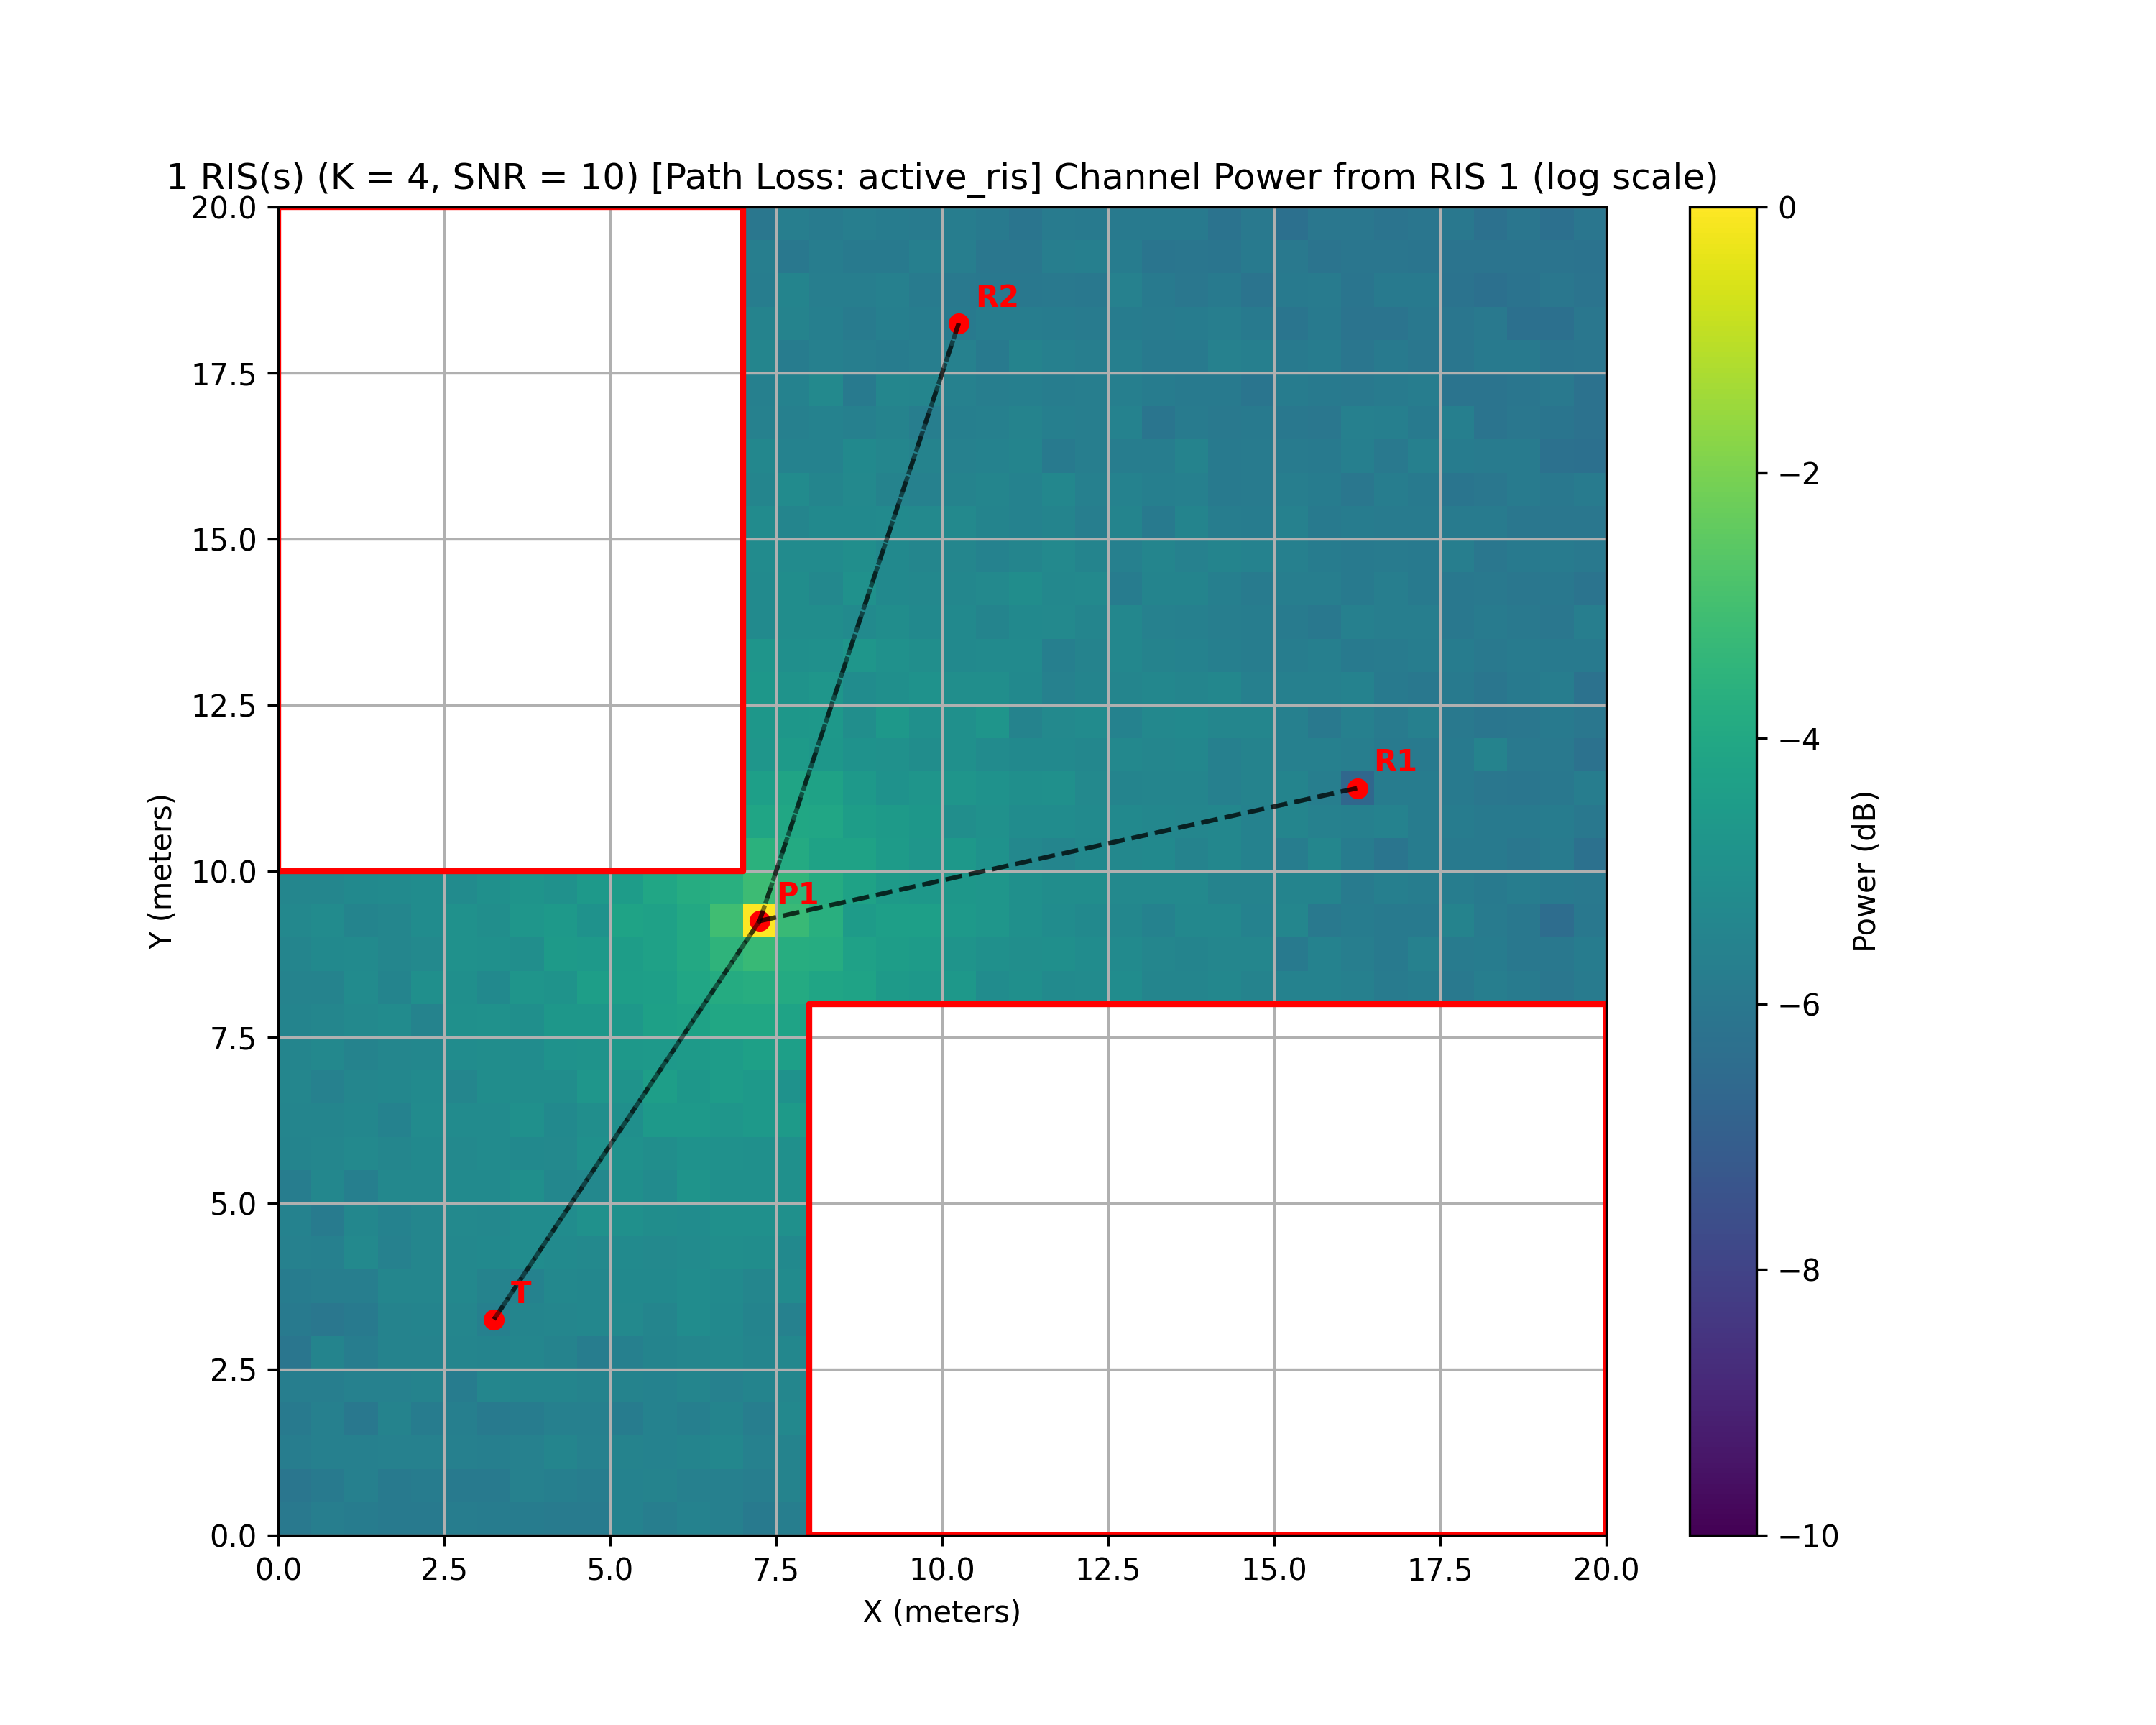
\includegraphics[width=0.8\linewidth]{imgs/heatmap-simulations/1 RIS(s) (K = 4, SNR = 10) [Path Loss_ active_ris] Channel Power from RIS 1 (log scale).png}
%   \caption{1 RIS(s) (K = 4, SNR = 10) [Path Loss: active ris] Channel Power from RIS 1 (log scale)}
% \end{figure}

% \begin{figure}[H]
%   \centering
%   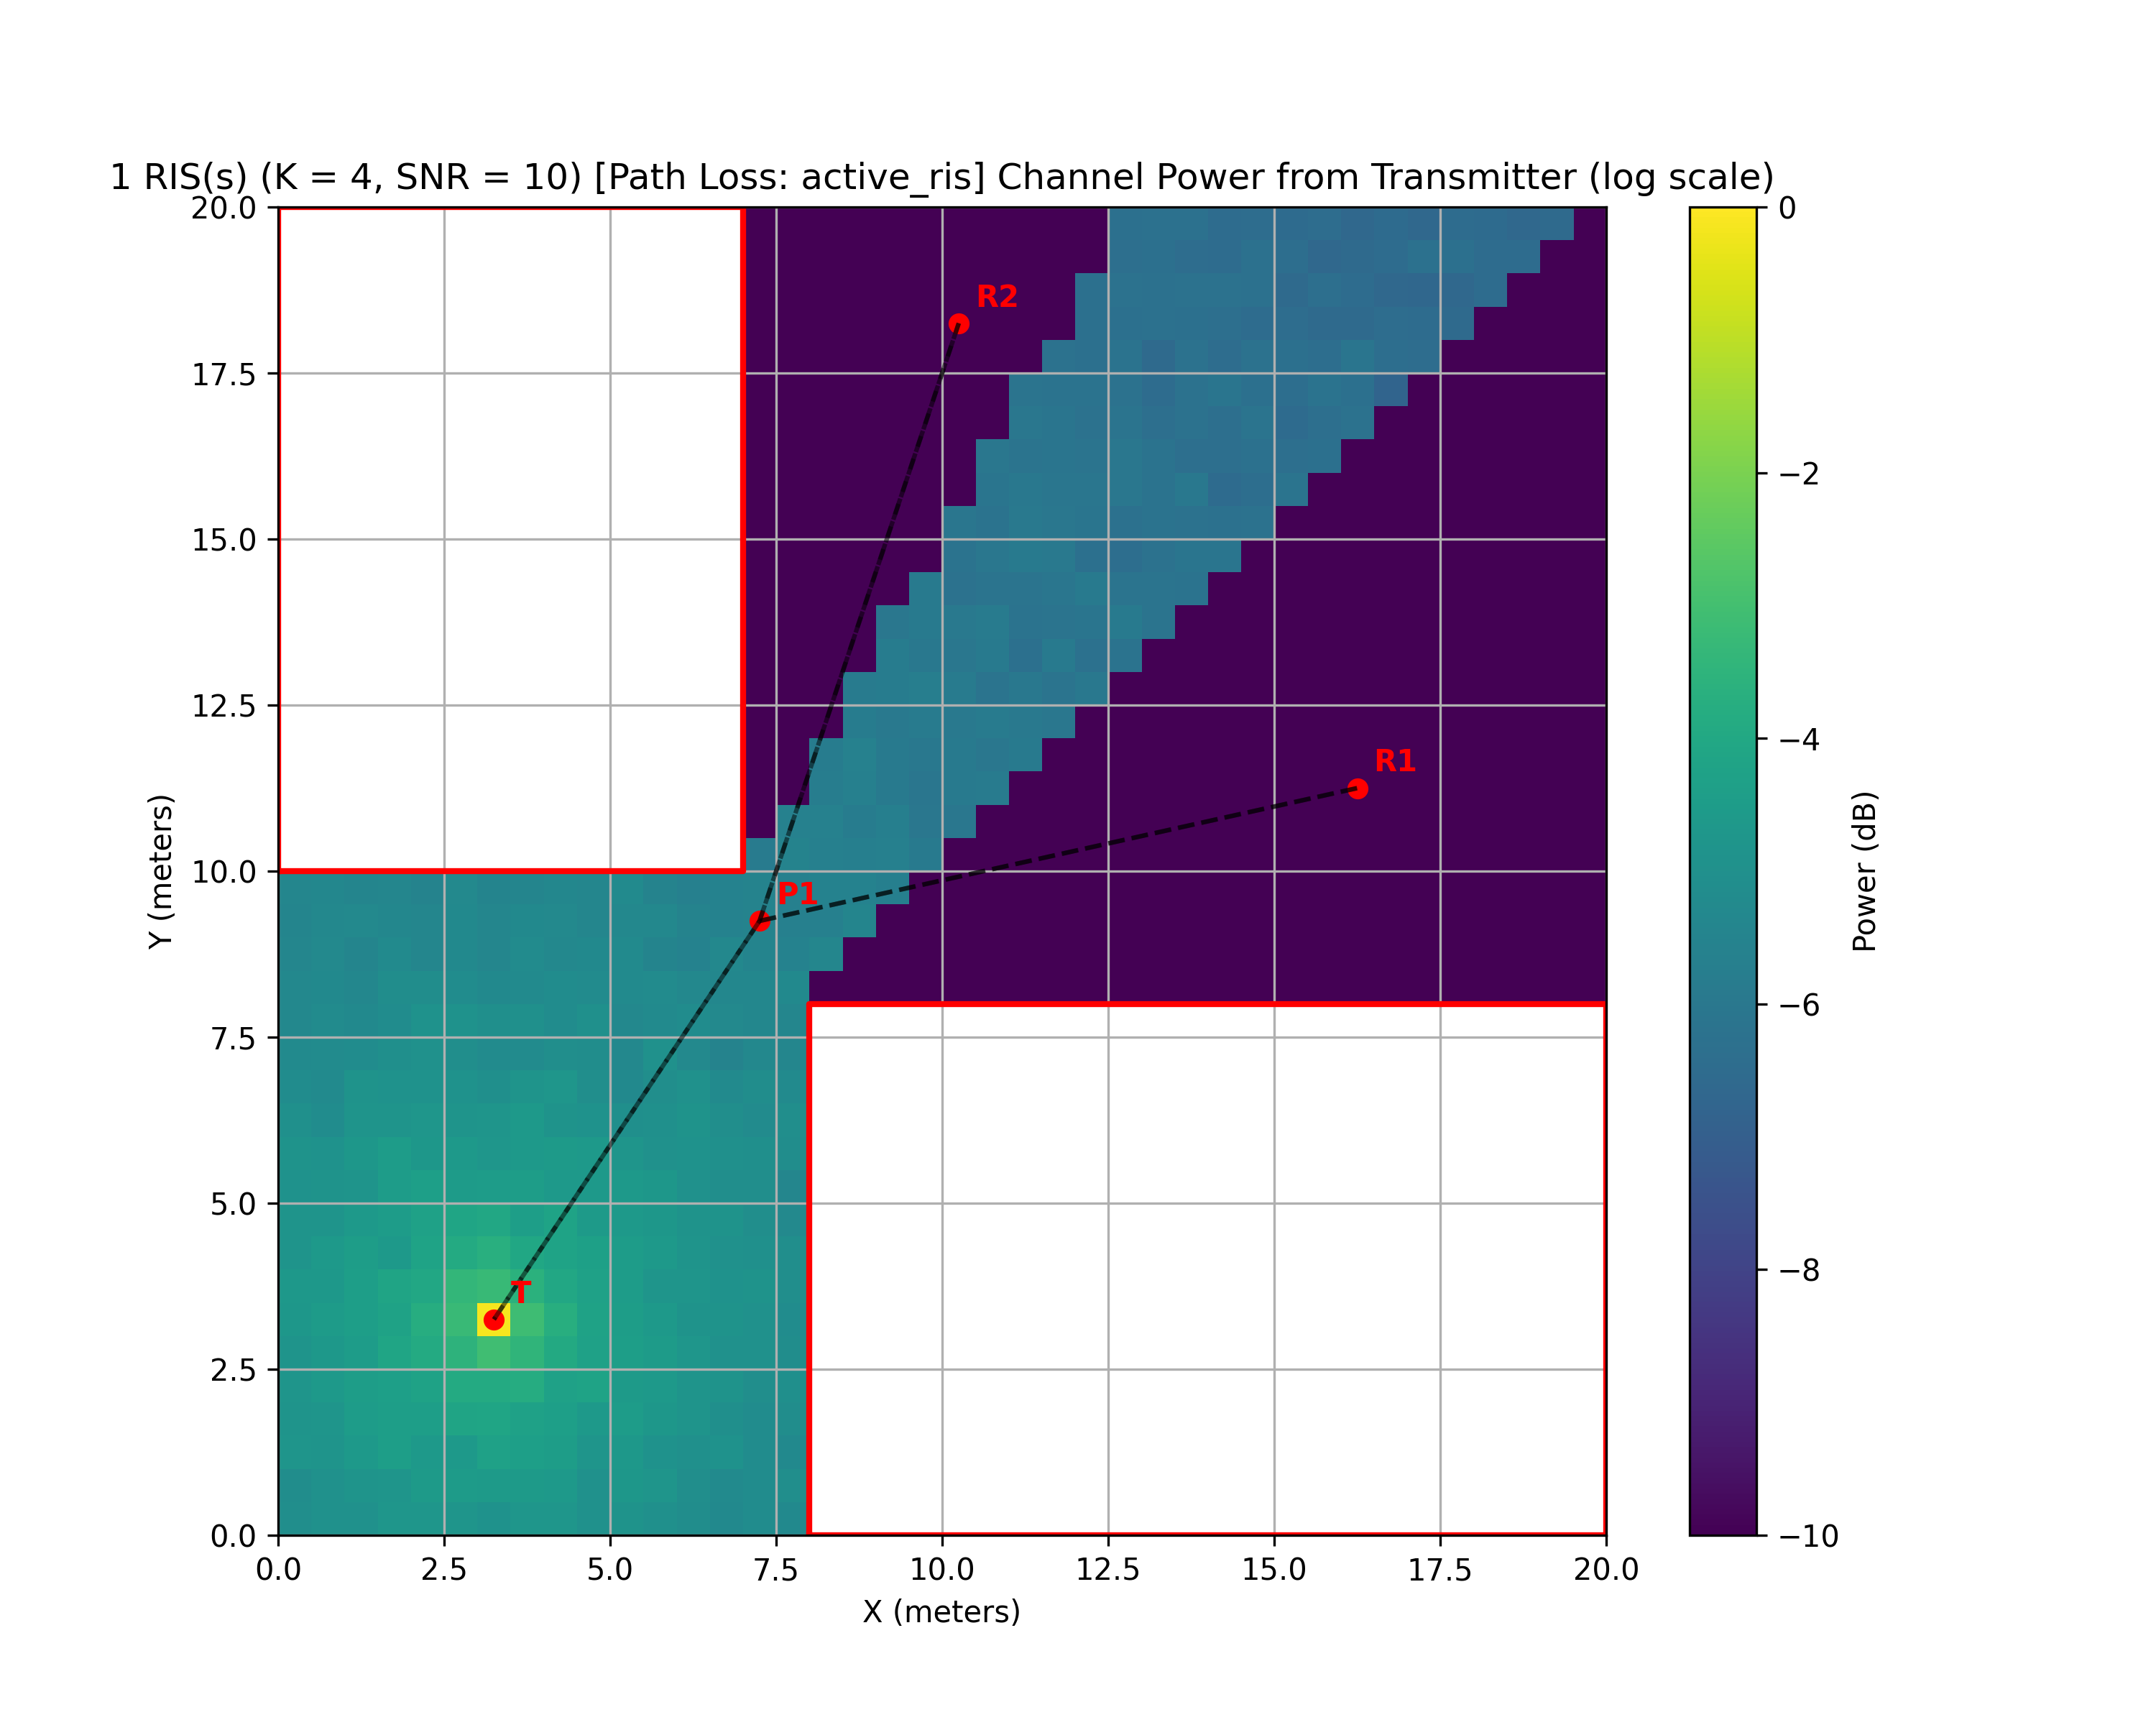
\includegraphics[width=0.8\linewidth]{imgs/heatmap-simulations/1 RIS(s) (K = 4, SNR = 10) [Path Loss_ active_ris] Channel Power from Transmitter (log scale).png}
%   \caption{1 RIS(s) (K = 4, SNR = 10) [Path Loss: active ris] Channel Power from Transmitter (log scale)}
% \end{figure}

% \begin{figure}[H]
%   \centering
%   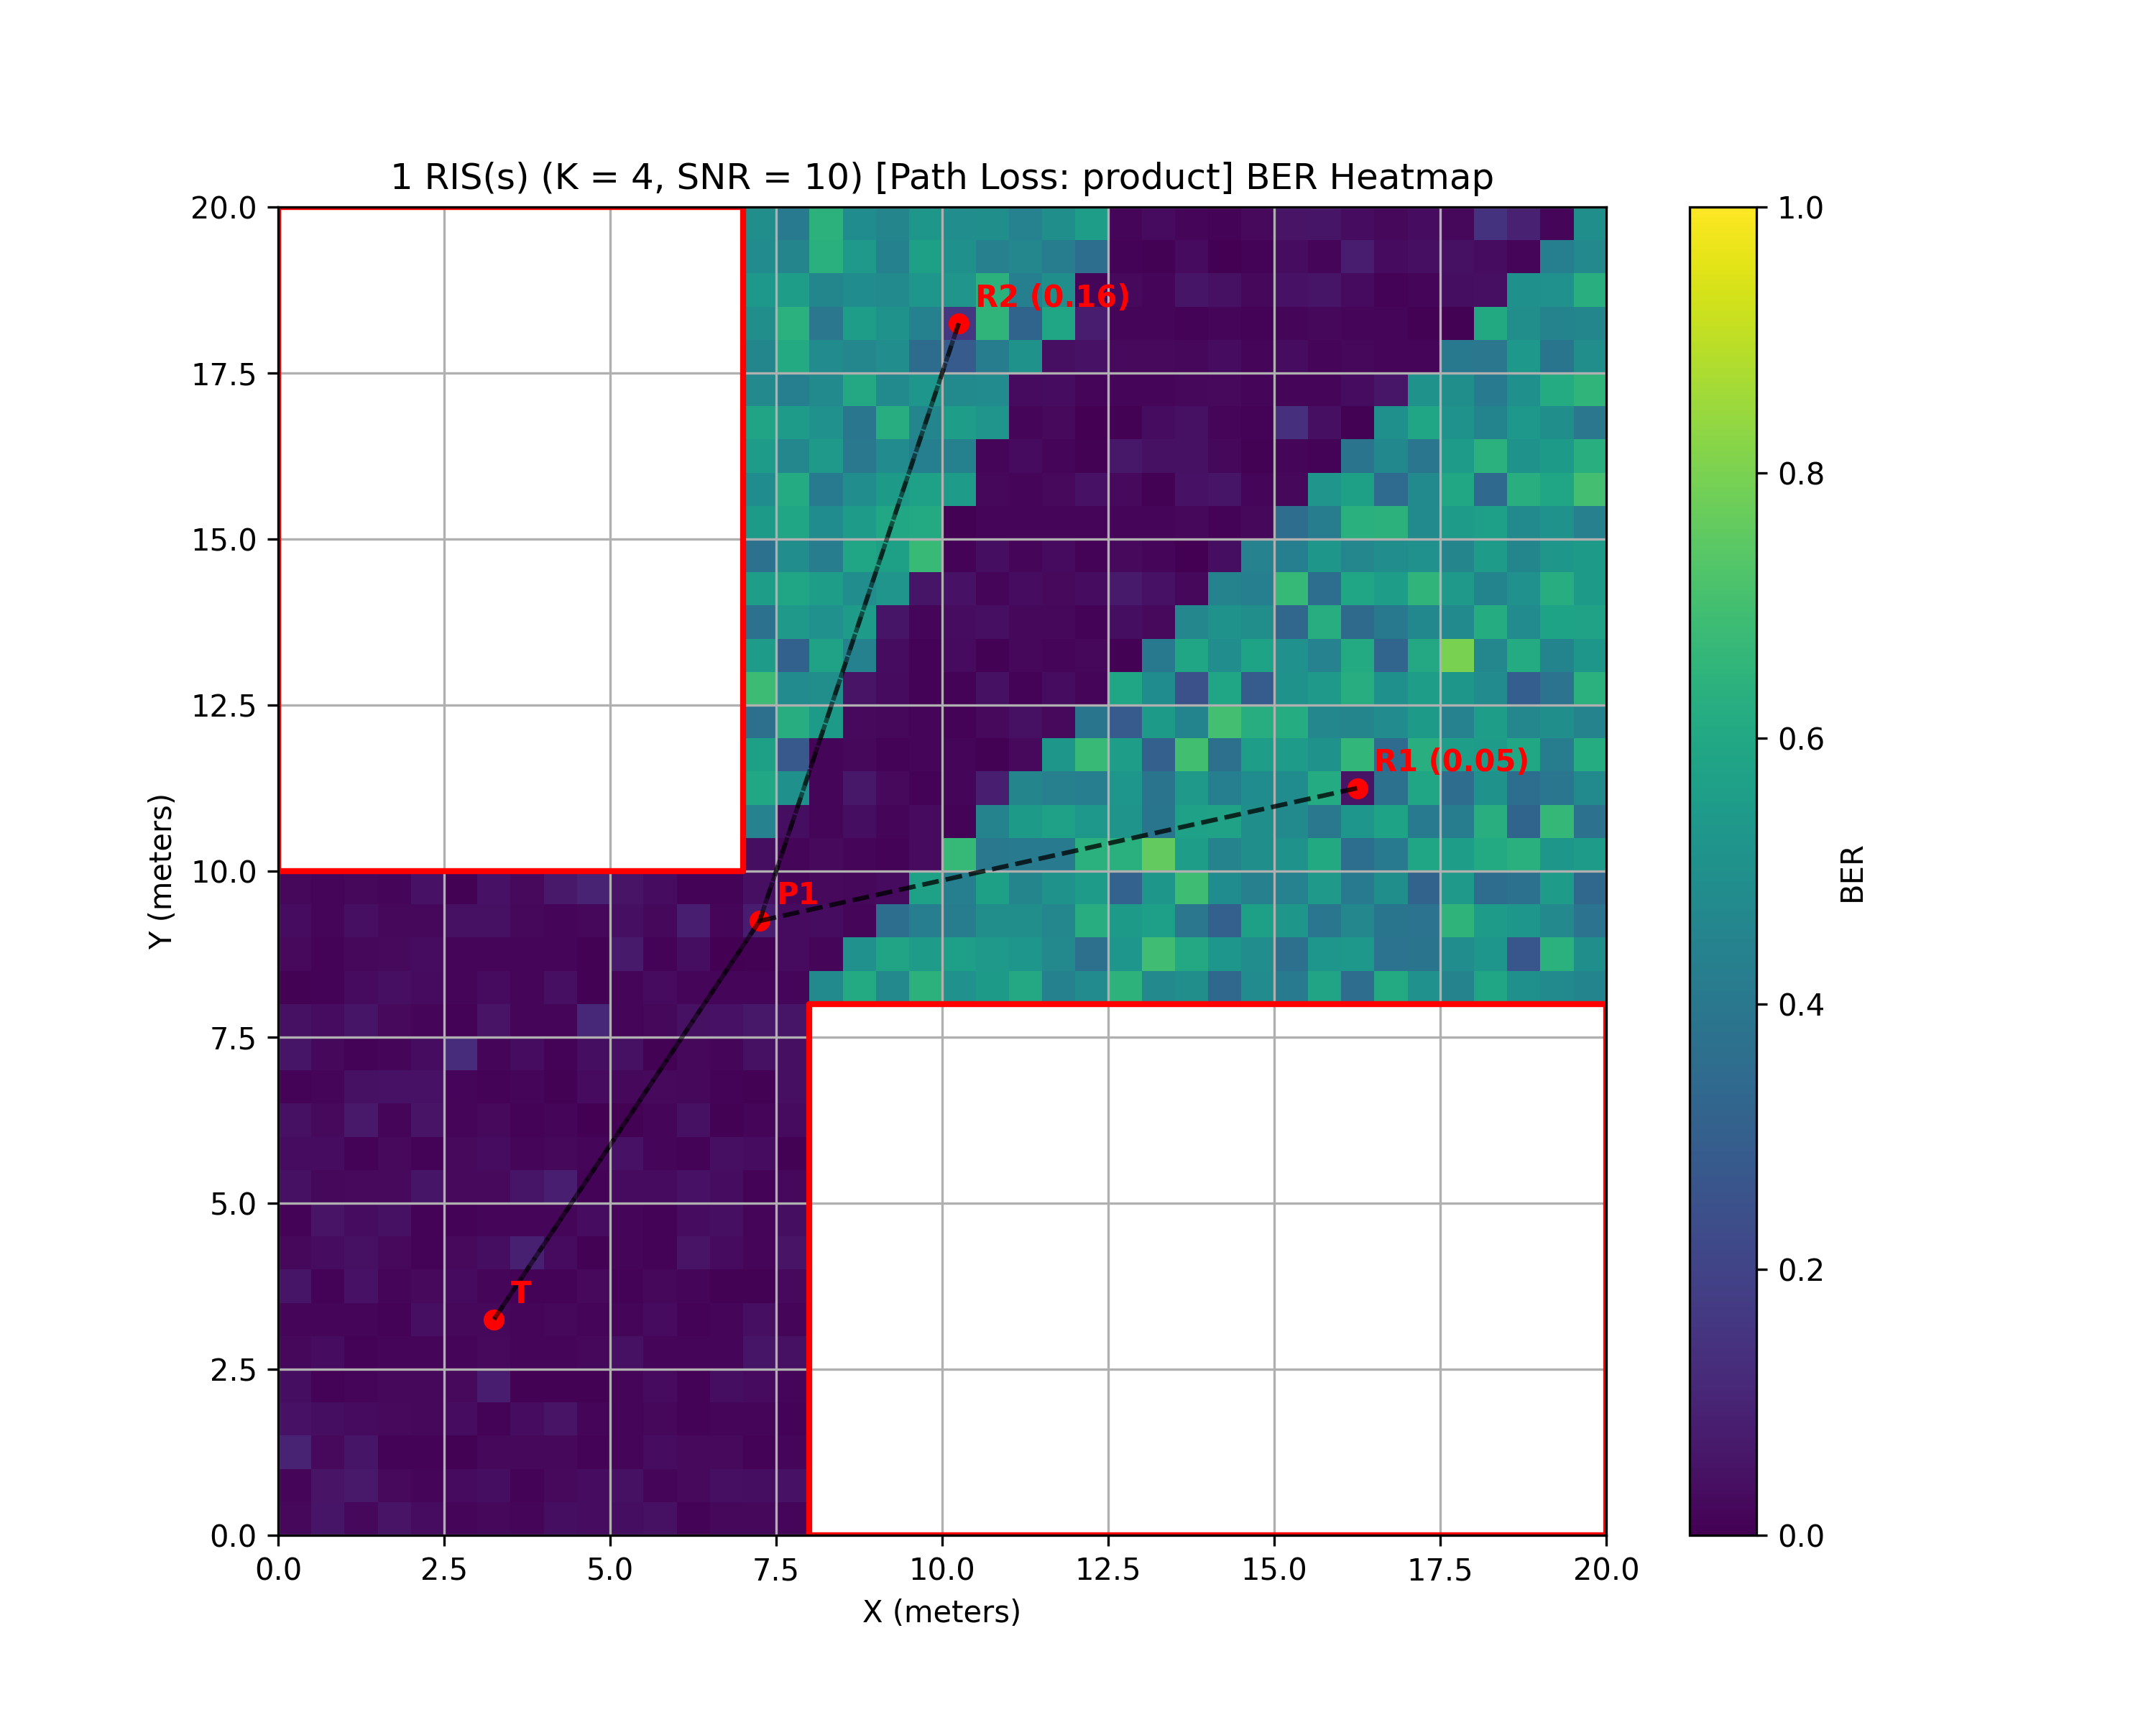
\includegraphics[width=0.8\linewidth]{imgs/heatmap-simulations/1 RIS(s) (K = 4, SNR = 10) [Path Loss_ product] BER Heatmap.png}
%   \caption{1 RIS(s) (K = 4, SNR = 10) [Path Loss: product] BER Heatmap}
% \end{figure}

% \begin{figure}[H]
%   \centering
%   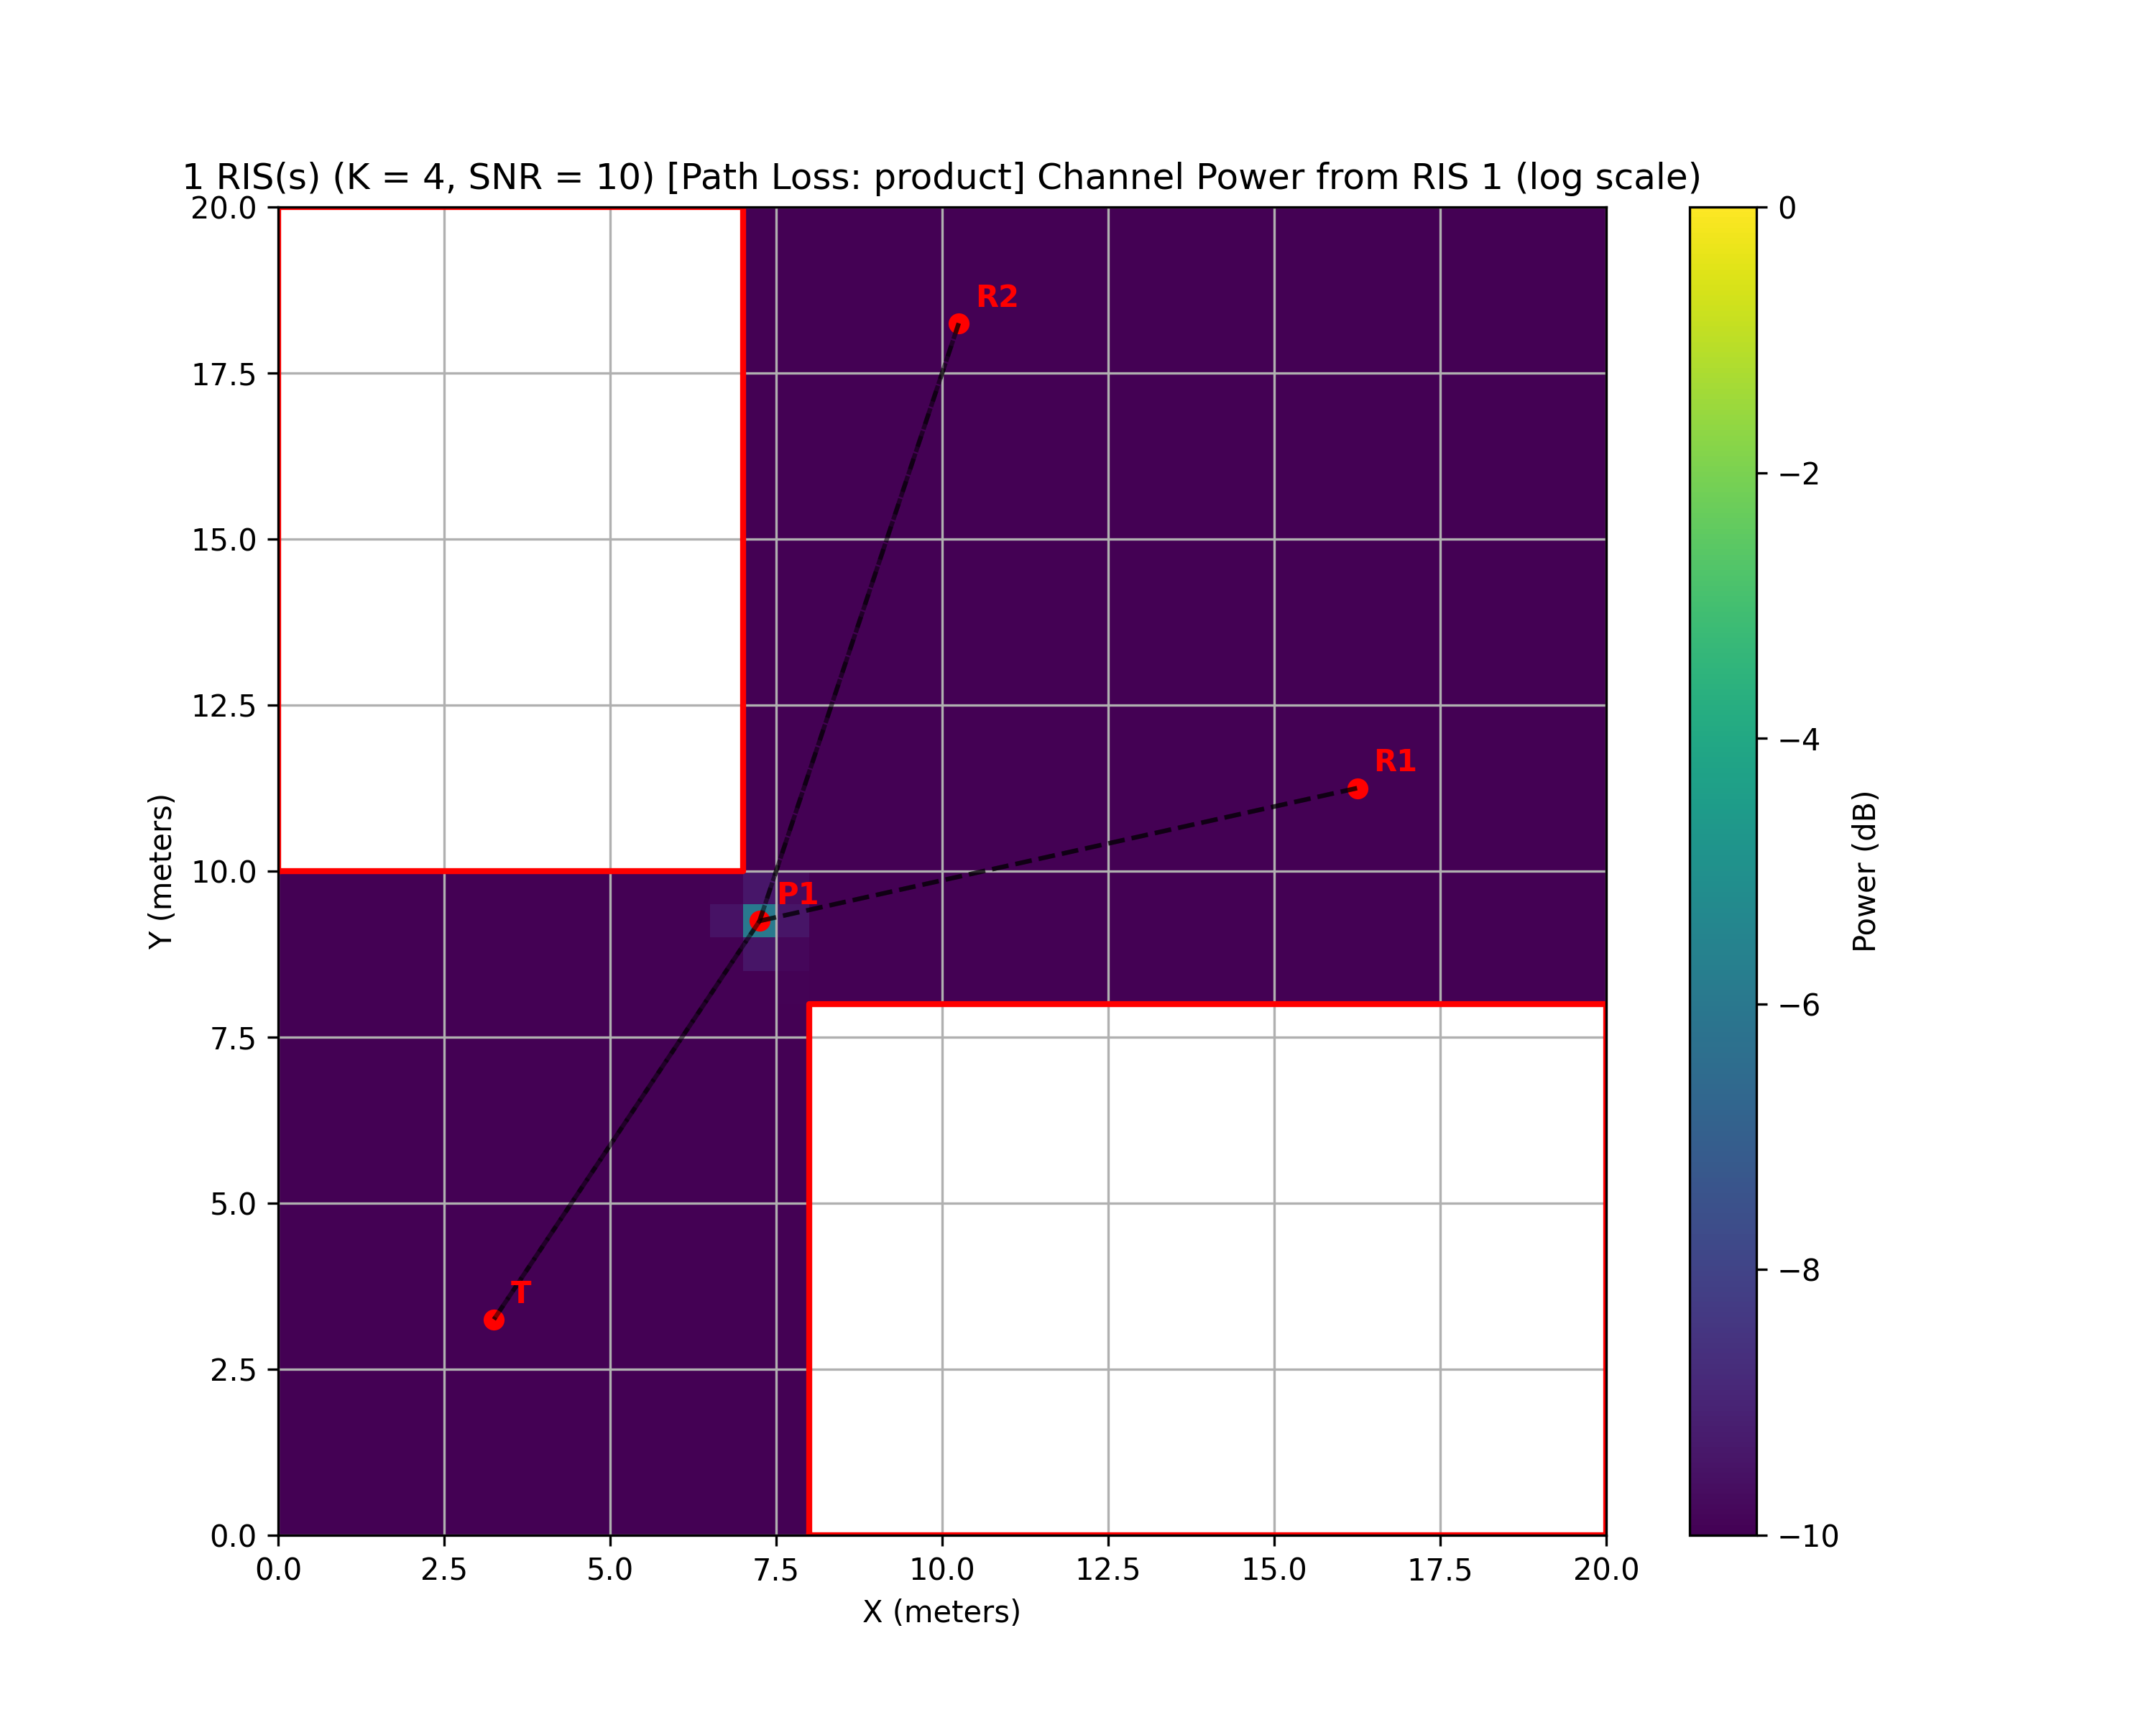
\includegraphics[width=0.8\linewidth]{imgs/heatmap-simulations/1 RIS(s) (K = 4, SNR = 10) [Path Loss_ product] Channel Power from RIS 1 (log scale).png}
%   \caption{1 RIS(s) (K = 4, SNR = 10) [Path Loss: product] Channel Power from RIS 1 (log scale)}
% \end{figure}

% \begin{figure}[H]
%   \centering
%   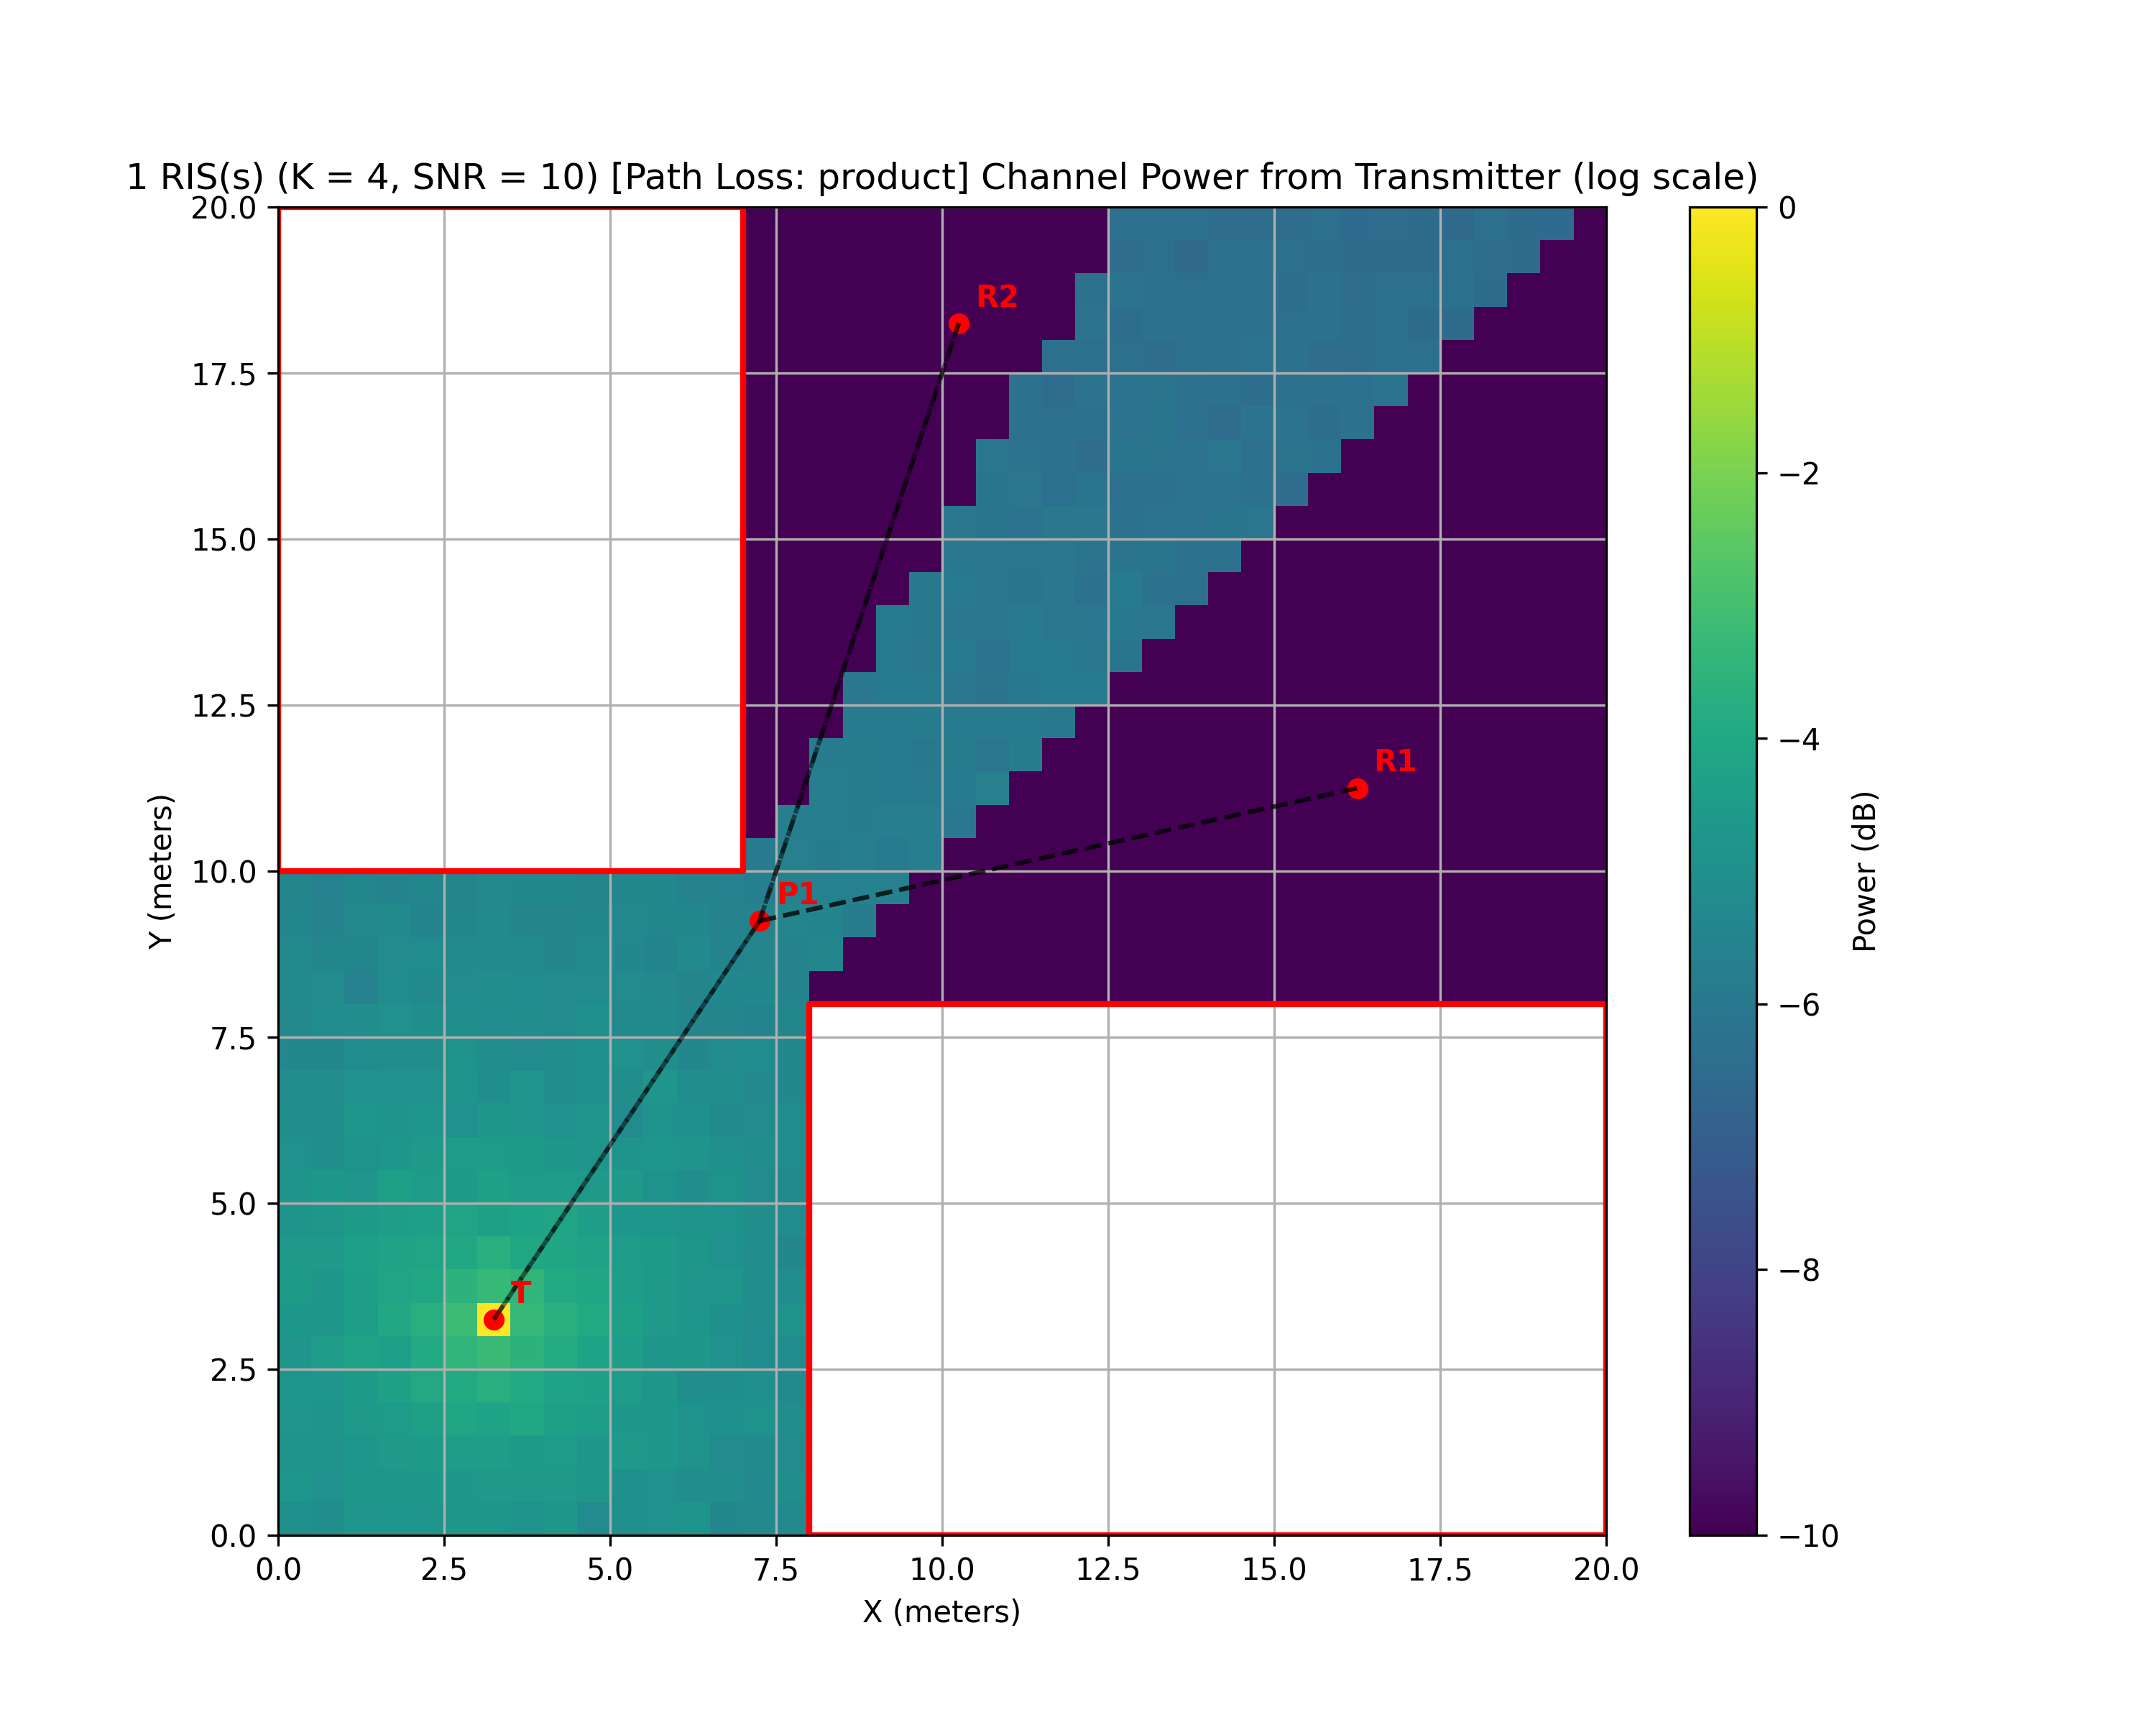
\includegraphics[width=0.8\linewidth]{imgs/heatmap-simulations/1 RIS(s) (K = 4, SNR = 10) [Path Loss_ product] Channel Power from Transmitter (log scale).png}
%   \caption{1 RIS(s) (K = 4, SNR = 10) [Path Loss: product] Channel Power from Transmitter (log scale)}
% \end{figure}

% \begin{figure}[H]
%   \centering
%   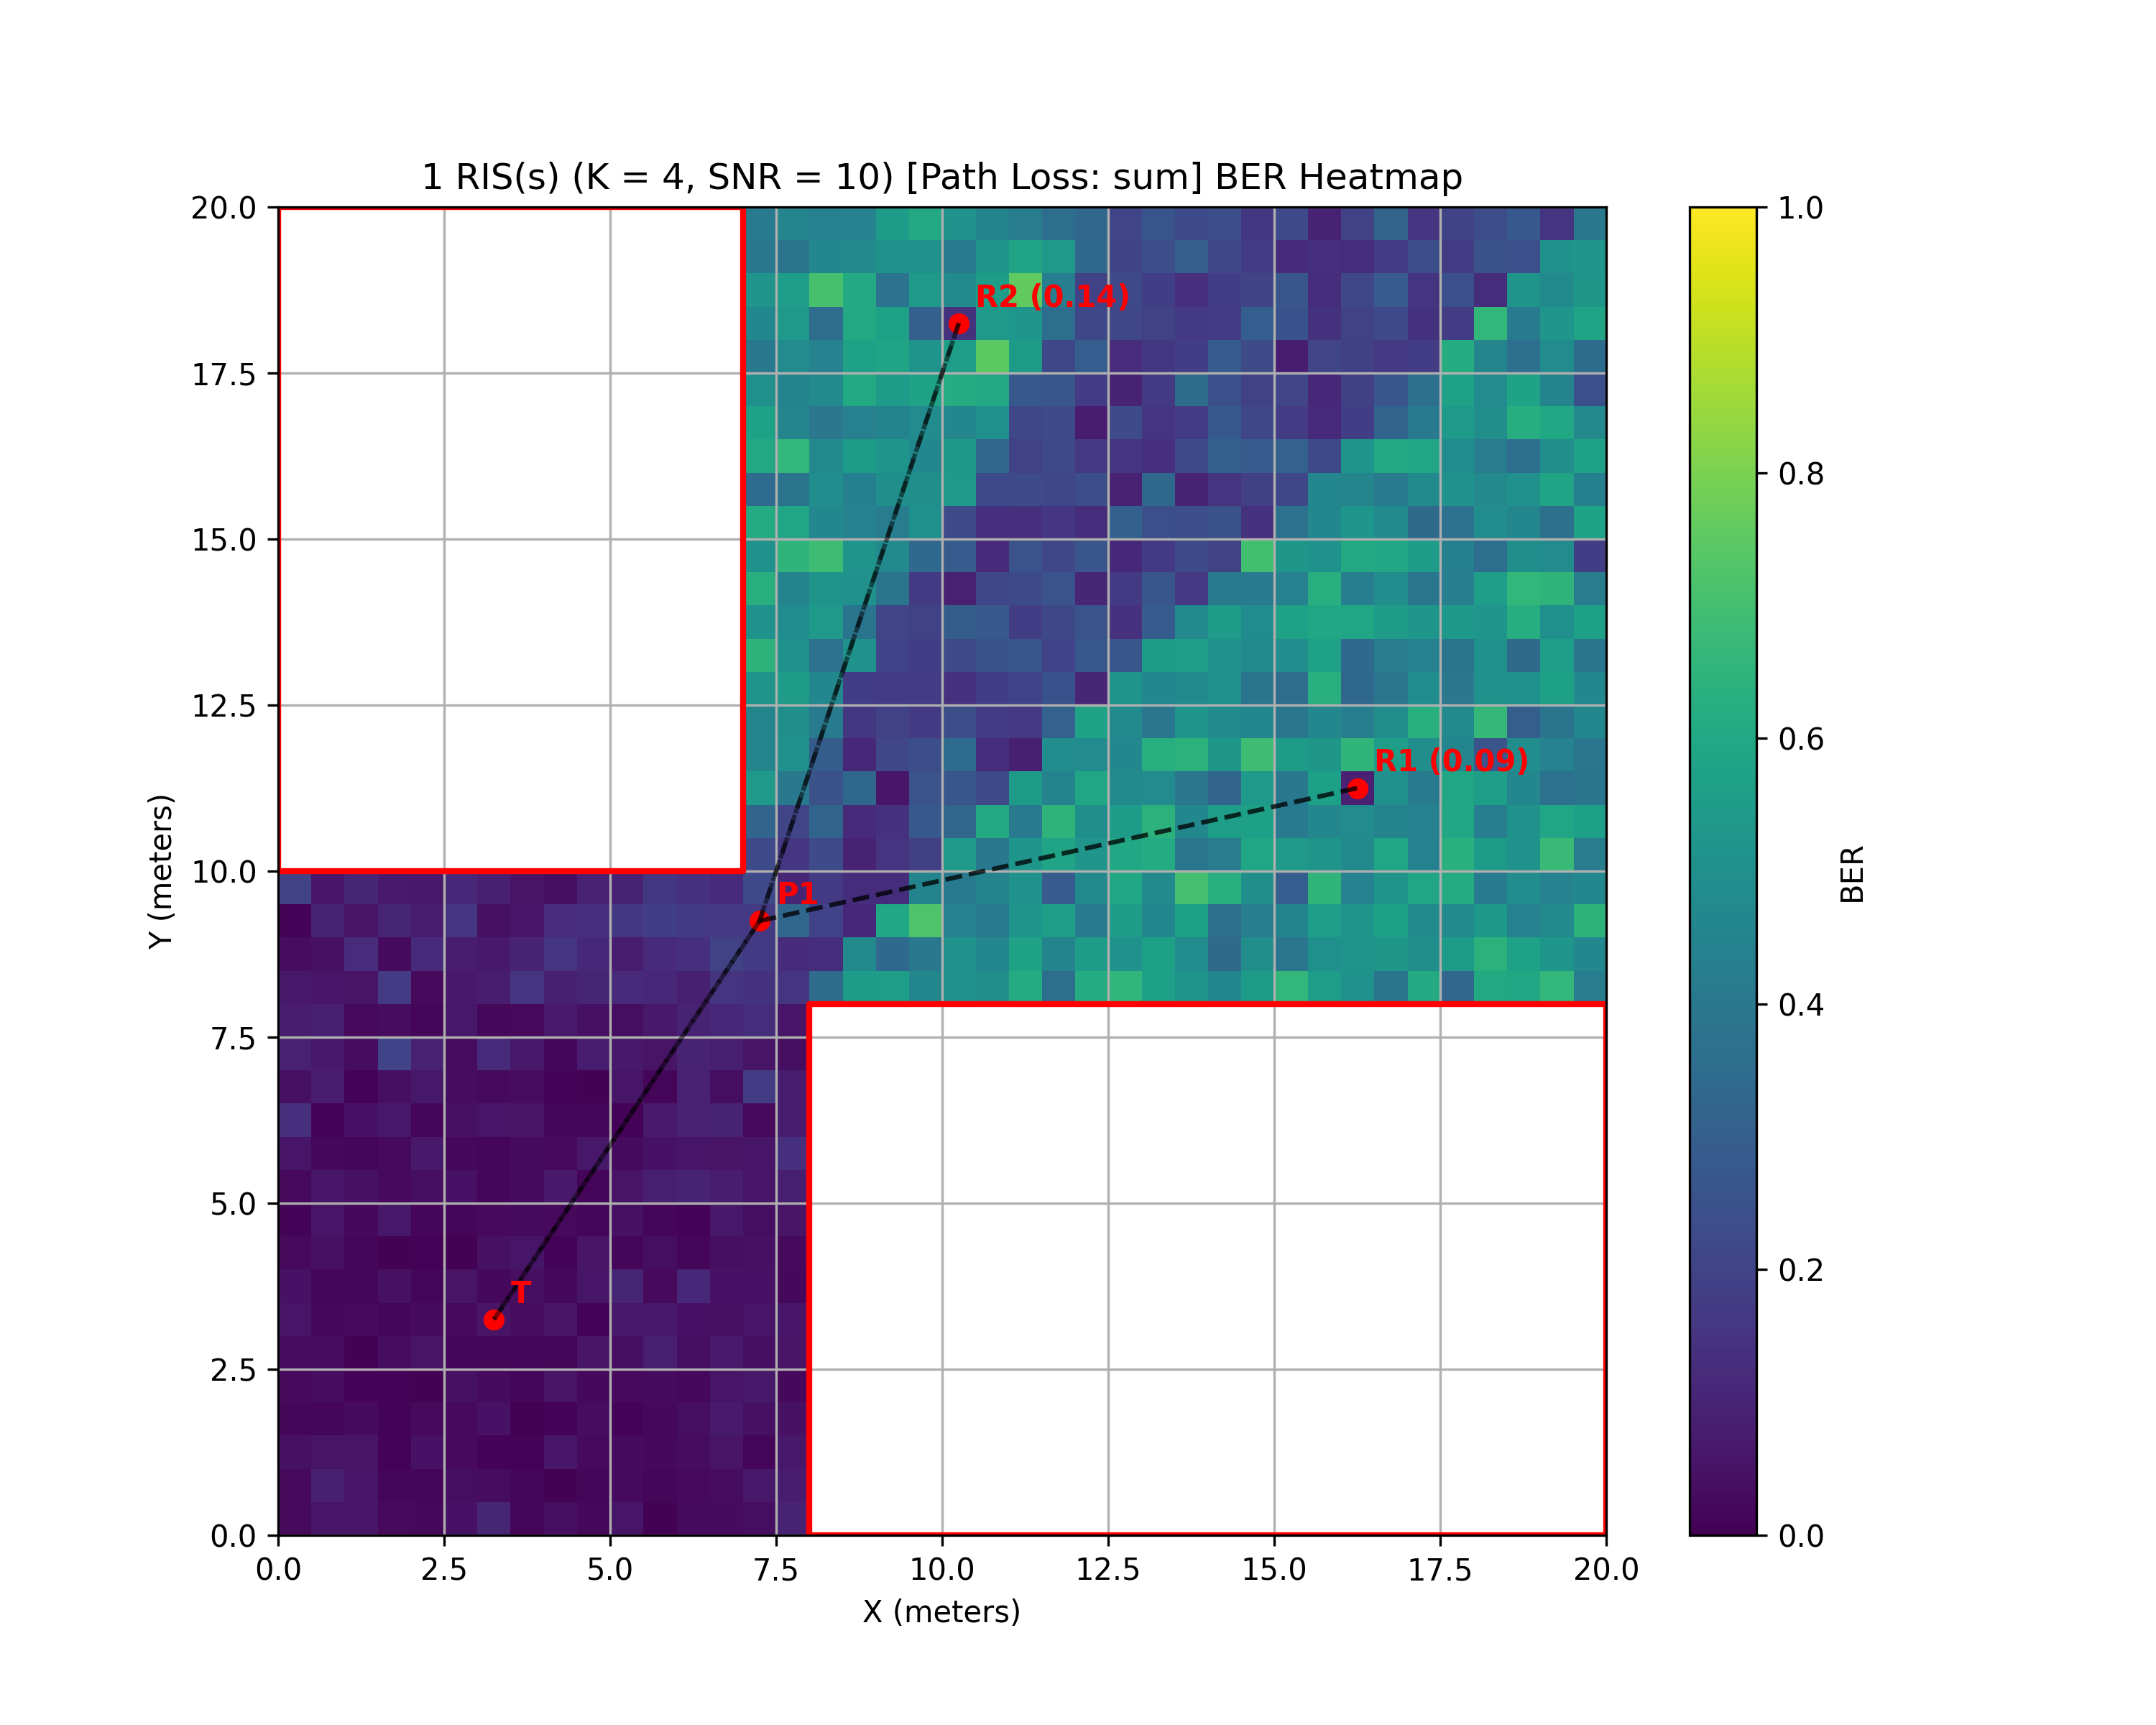
\includegraphics[width=0.8\linewidth]{imgs/heatmap-simulations/1 RIS(s) (K = 4, SNR = 10) [Path Loss_ sum] BER Heatmap.png}
%   \caption{1 RIS(s) (K = 4, SNR = 10) [Path Loss: sum] BER Heatmap}
% \end{figure}

% \begin{figure}[H]
%   \centering
%   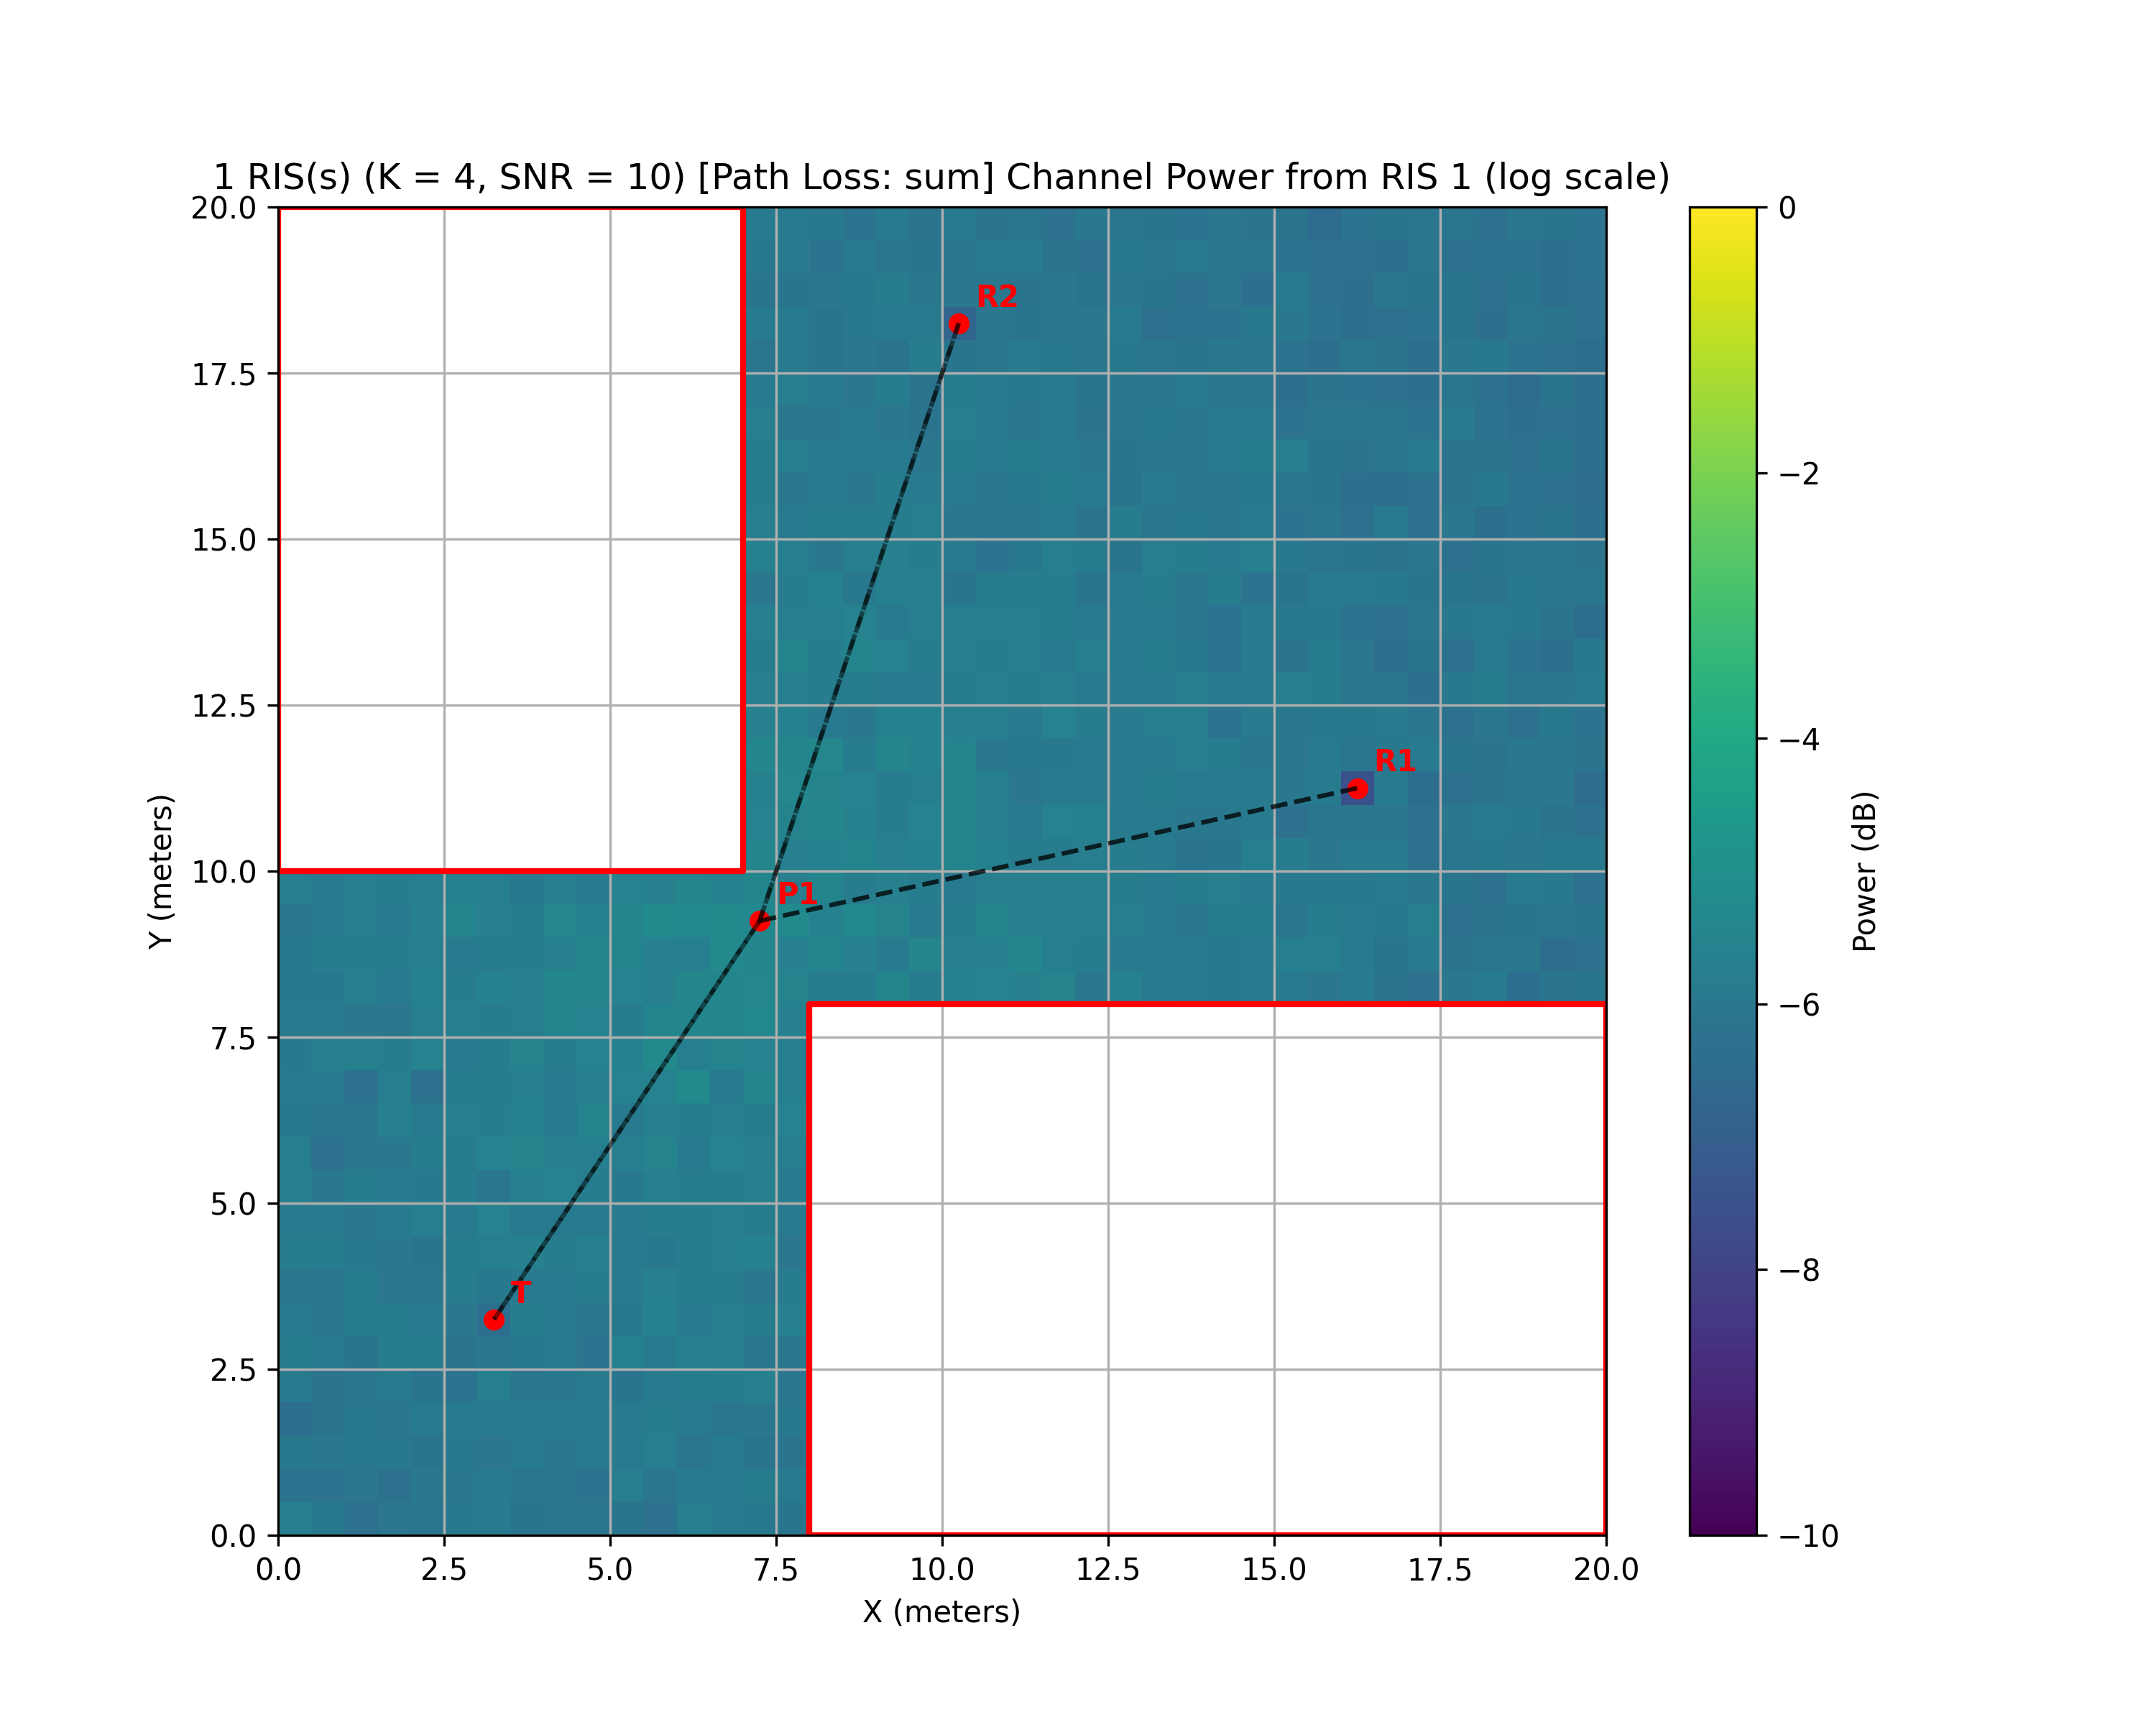
\includegraphics[width=0.8\linewidth]{imgs/heatmap-simulations/1 RIS(s) (K = 4, SNR = 10) [Path Loss_ sum] Channel Power from RIS 1 (log scale).png}
%   \caption{1 RIS(s) (K = 4, SNR = 10) [Path Loss: sum] Channel Power from RIS 1 (log scale)}
% \end{figure}

% \begin{figure}[H]
%   \centering
%   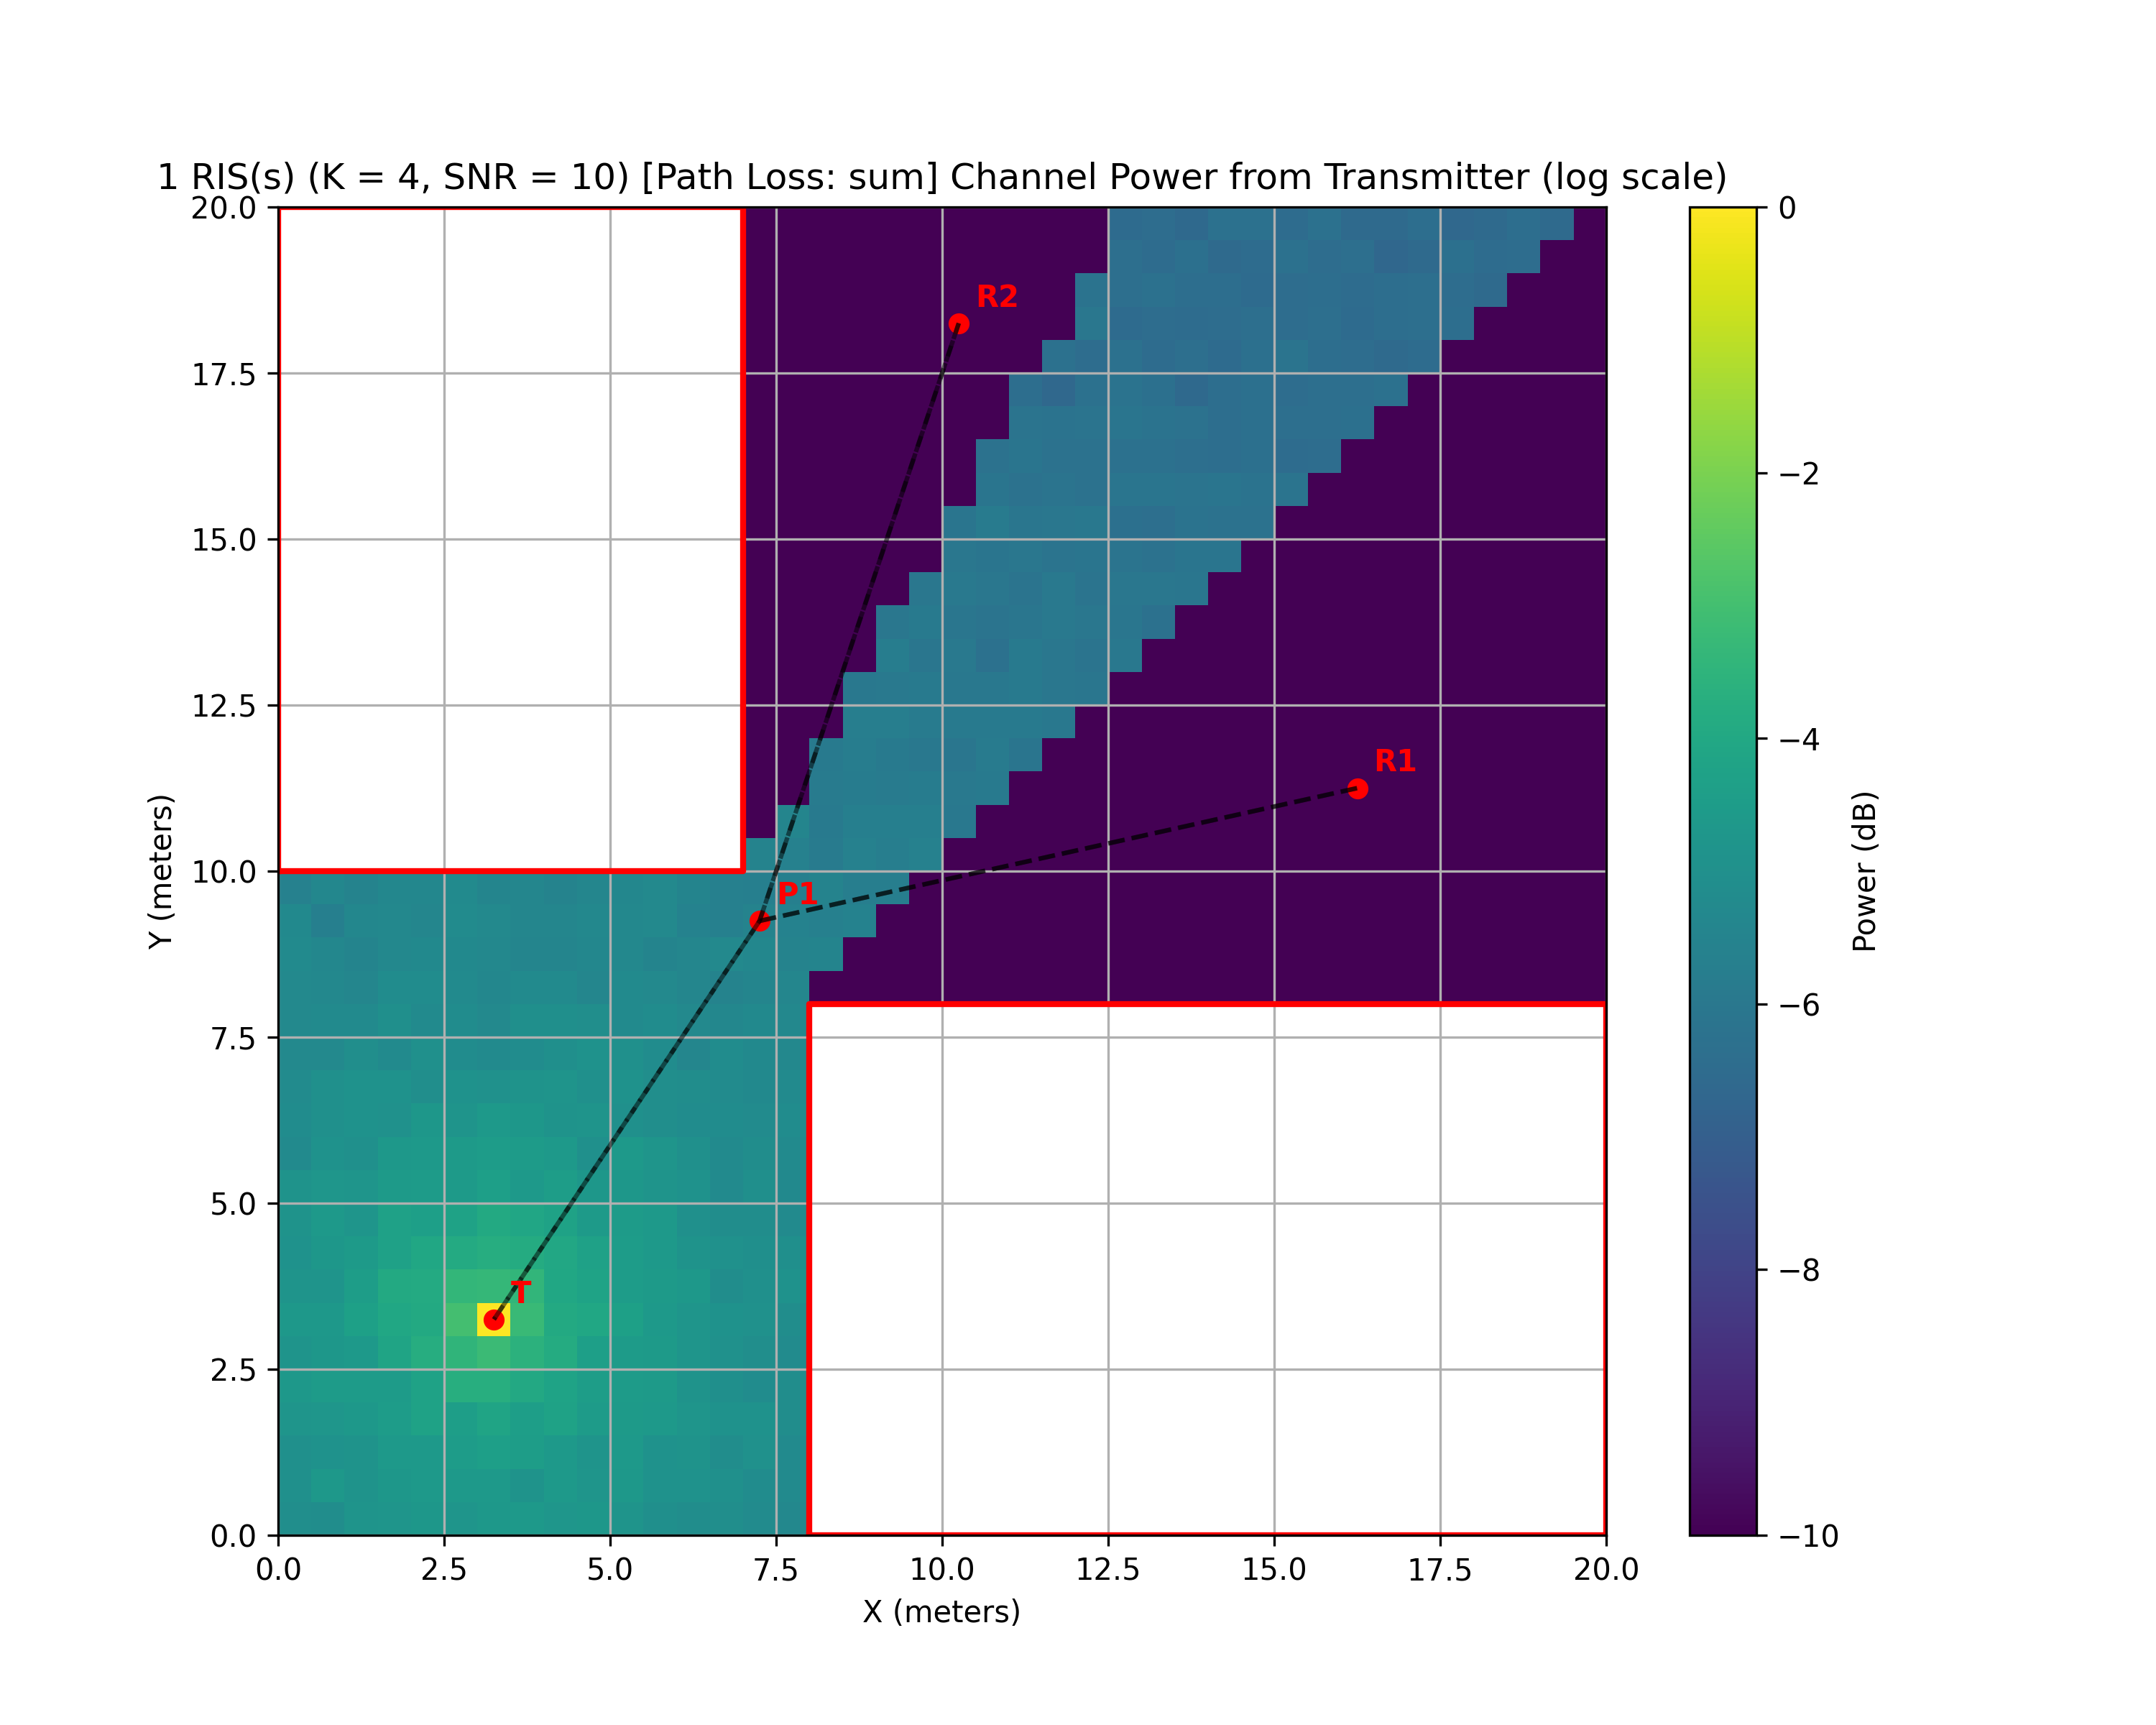
\includegraphics[width=0.8\linewidth]{imgs/heatmap-simulations/1 RIS(s) (K = 4, SNR = 10) [Path Loss_ sum] Channel Power from Transmitter (log scale).png}
%   \caption{1 RIS(s) (K = 4, SNR = 10) [Path Loss: sum] Channel Power from Transmitter (log scale)}
% \end{figure}

% \begin{figure}[H]
%   \centering
%   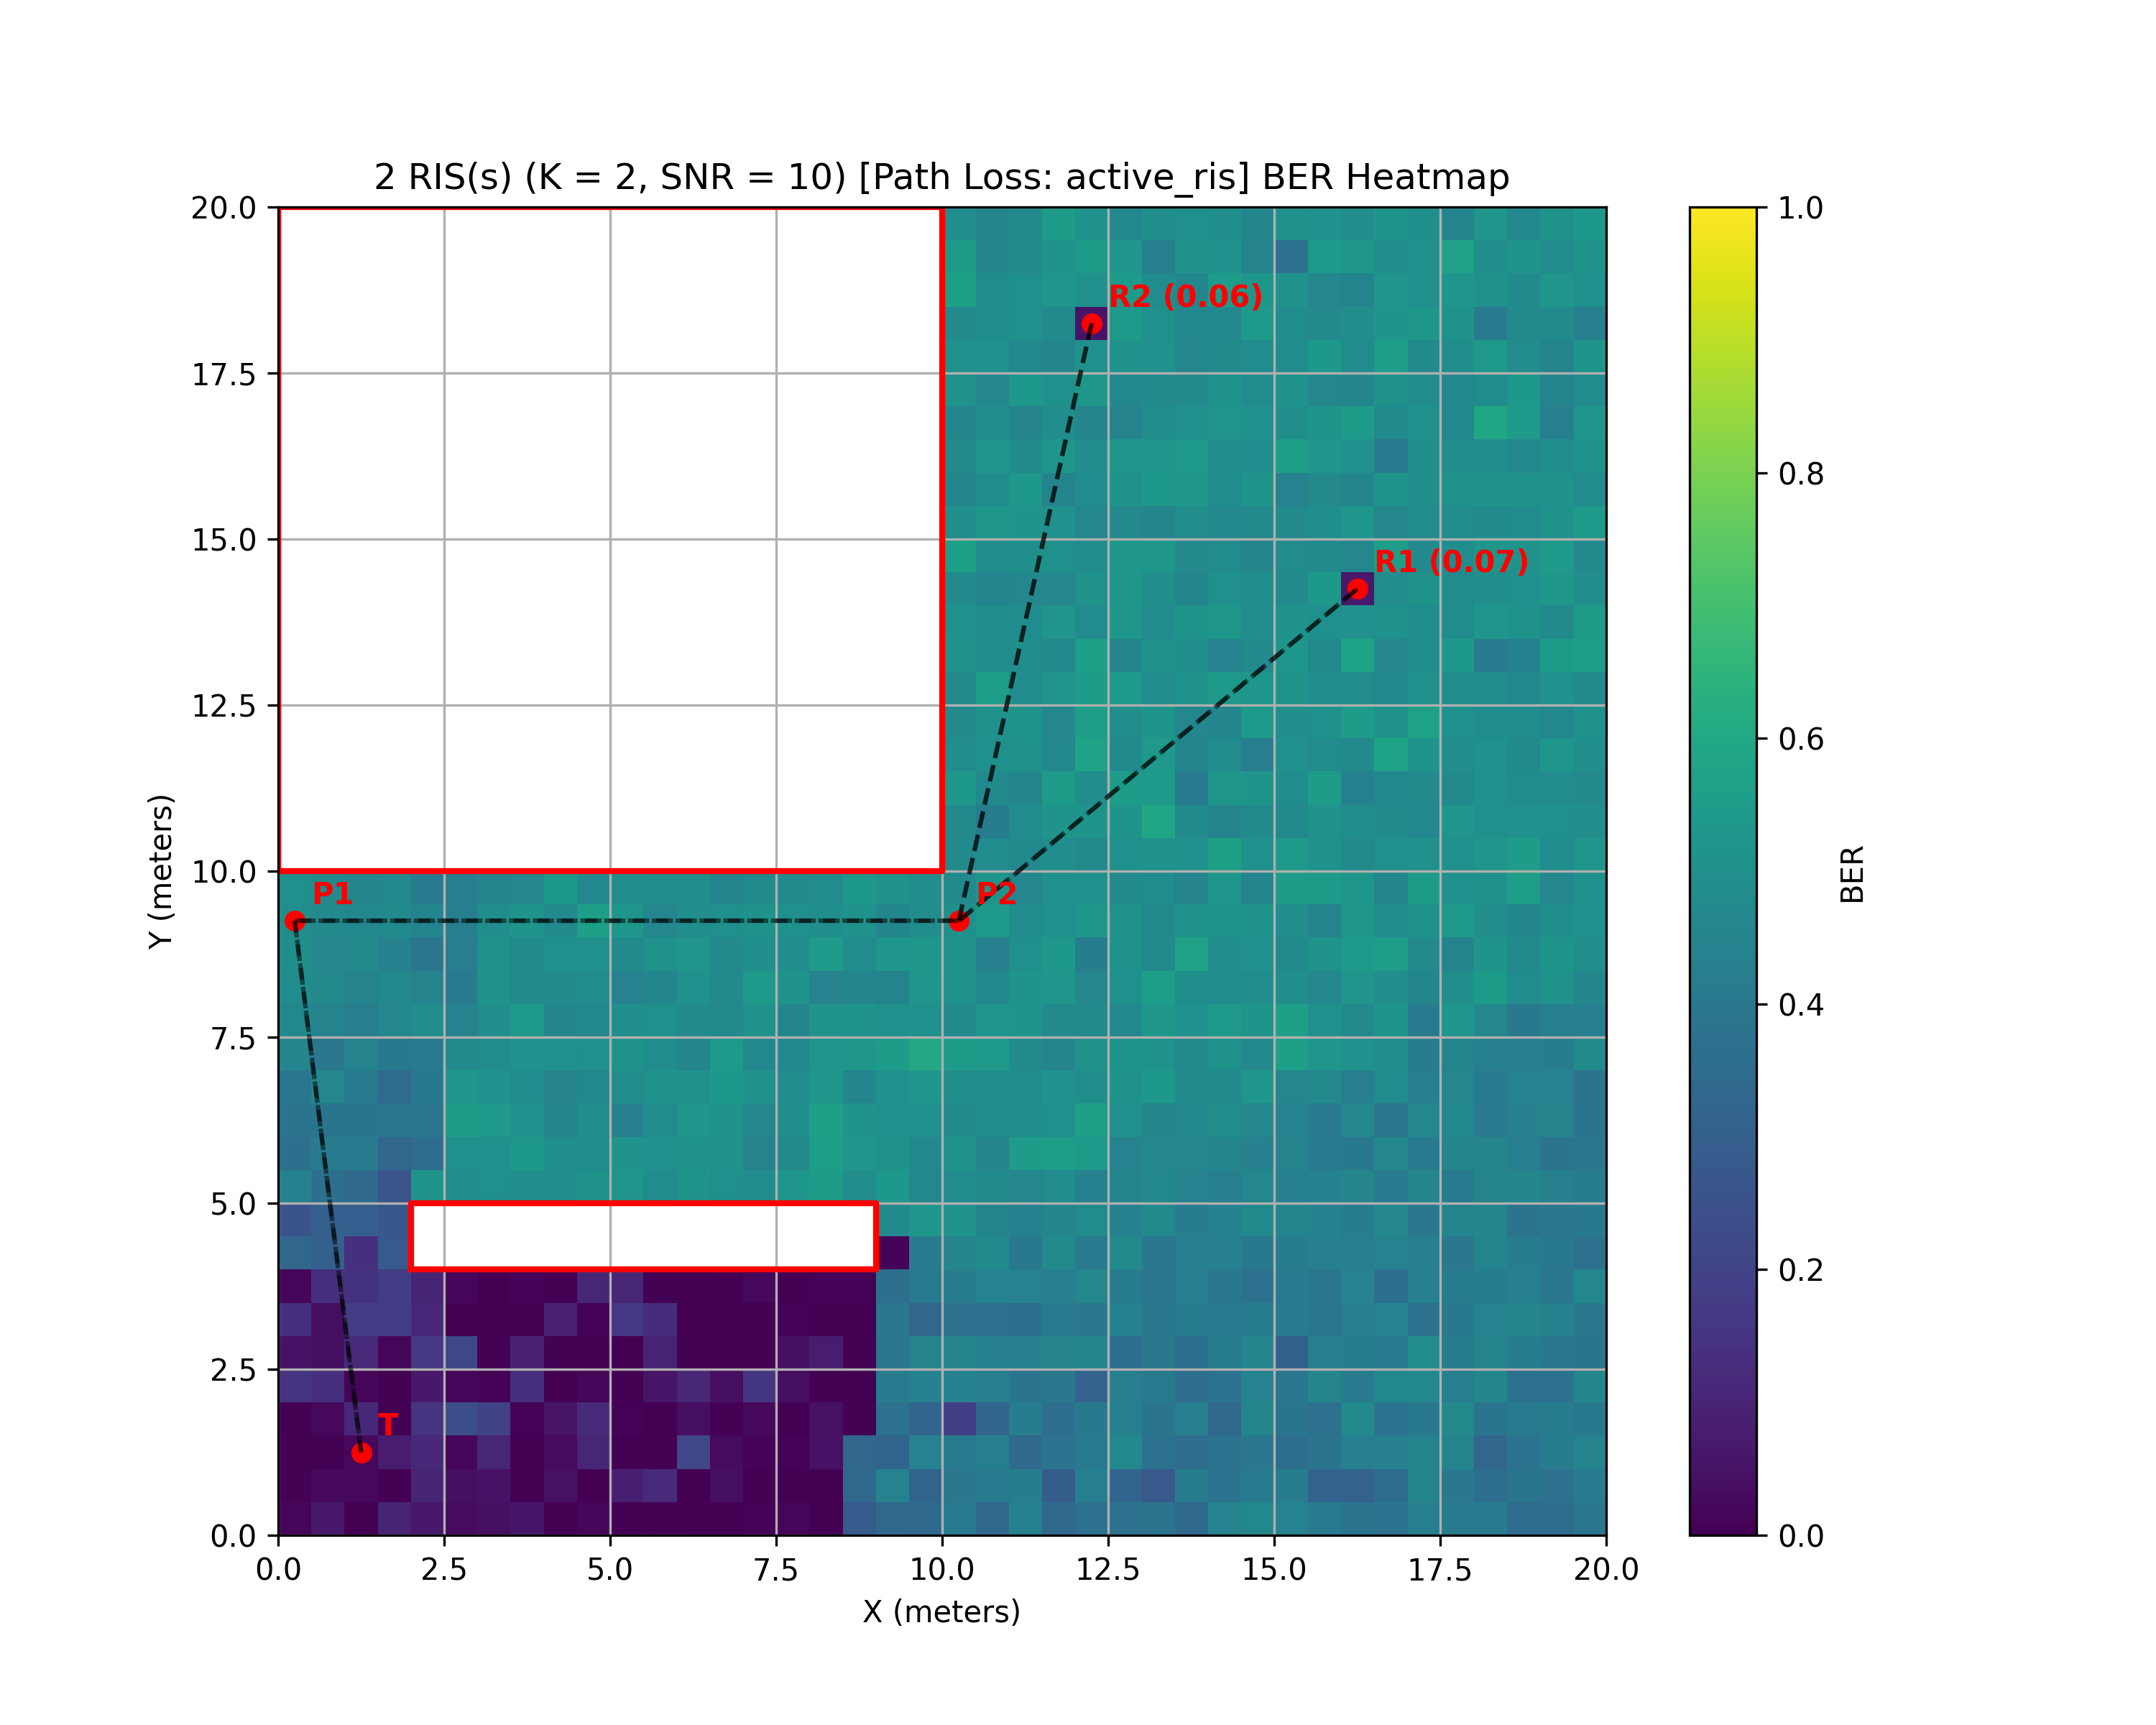
\includegraphics[width=0.8\linewidth]{imgs/heatmap-simulations/2 RIS(s) (K = 2, SNR = 10) [Path Loss_ active_ris] BER Heatmap.png}
%   \caption{2 RIS(s) (K = 2, SNR = 10) [Path Loss: active ris] BER Heatmap}
% \end{figure}

% \begin{figure}[H]
%   \centering
%   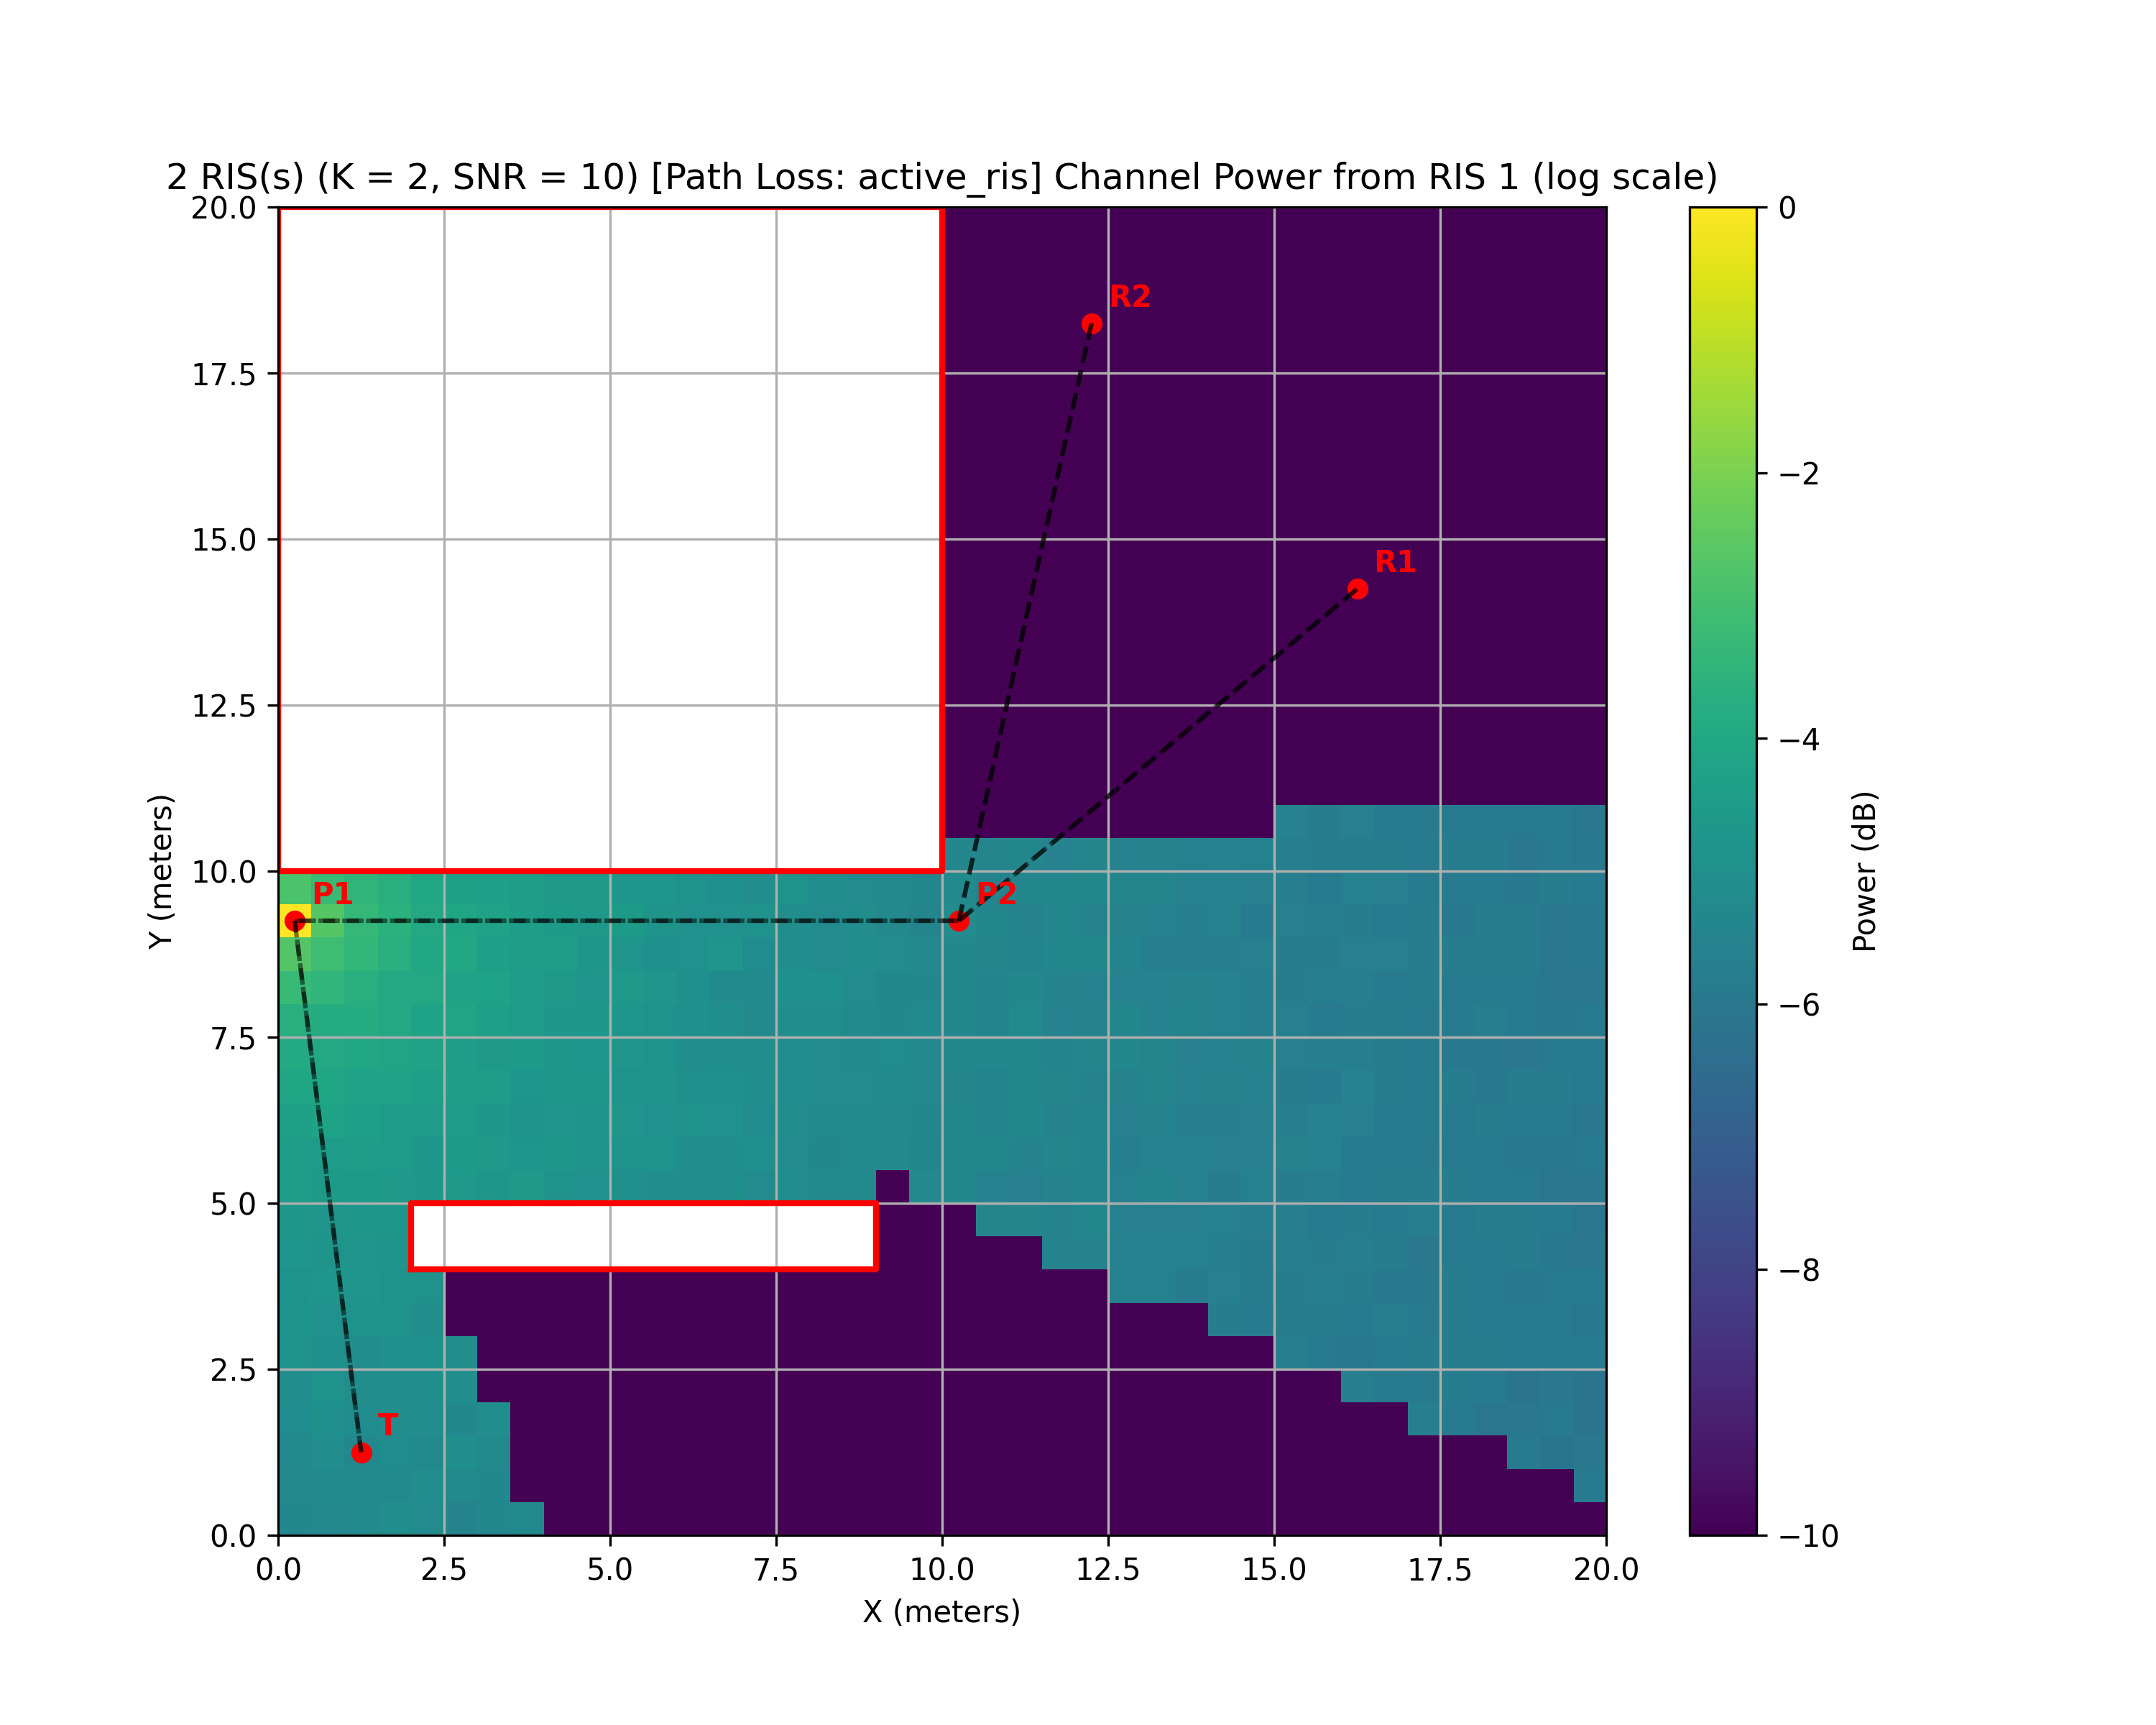
\includegraphics[width=0.8\linewidth]{imgs/heatmap-simulations/2 RIS(s) (K = 2, SNR = 10) [Path Loss_ active_ris] Channel Power from RIS 1 (log scale).png}
%   \caption{2 RIS(s) (K = 2, SNR = 10) [Path Loss: active ris] Channel Power from RIS 1 (log scale)}
% \end{figure}

% \begin{figure}[H]
%   \centering
%   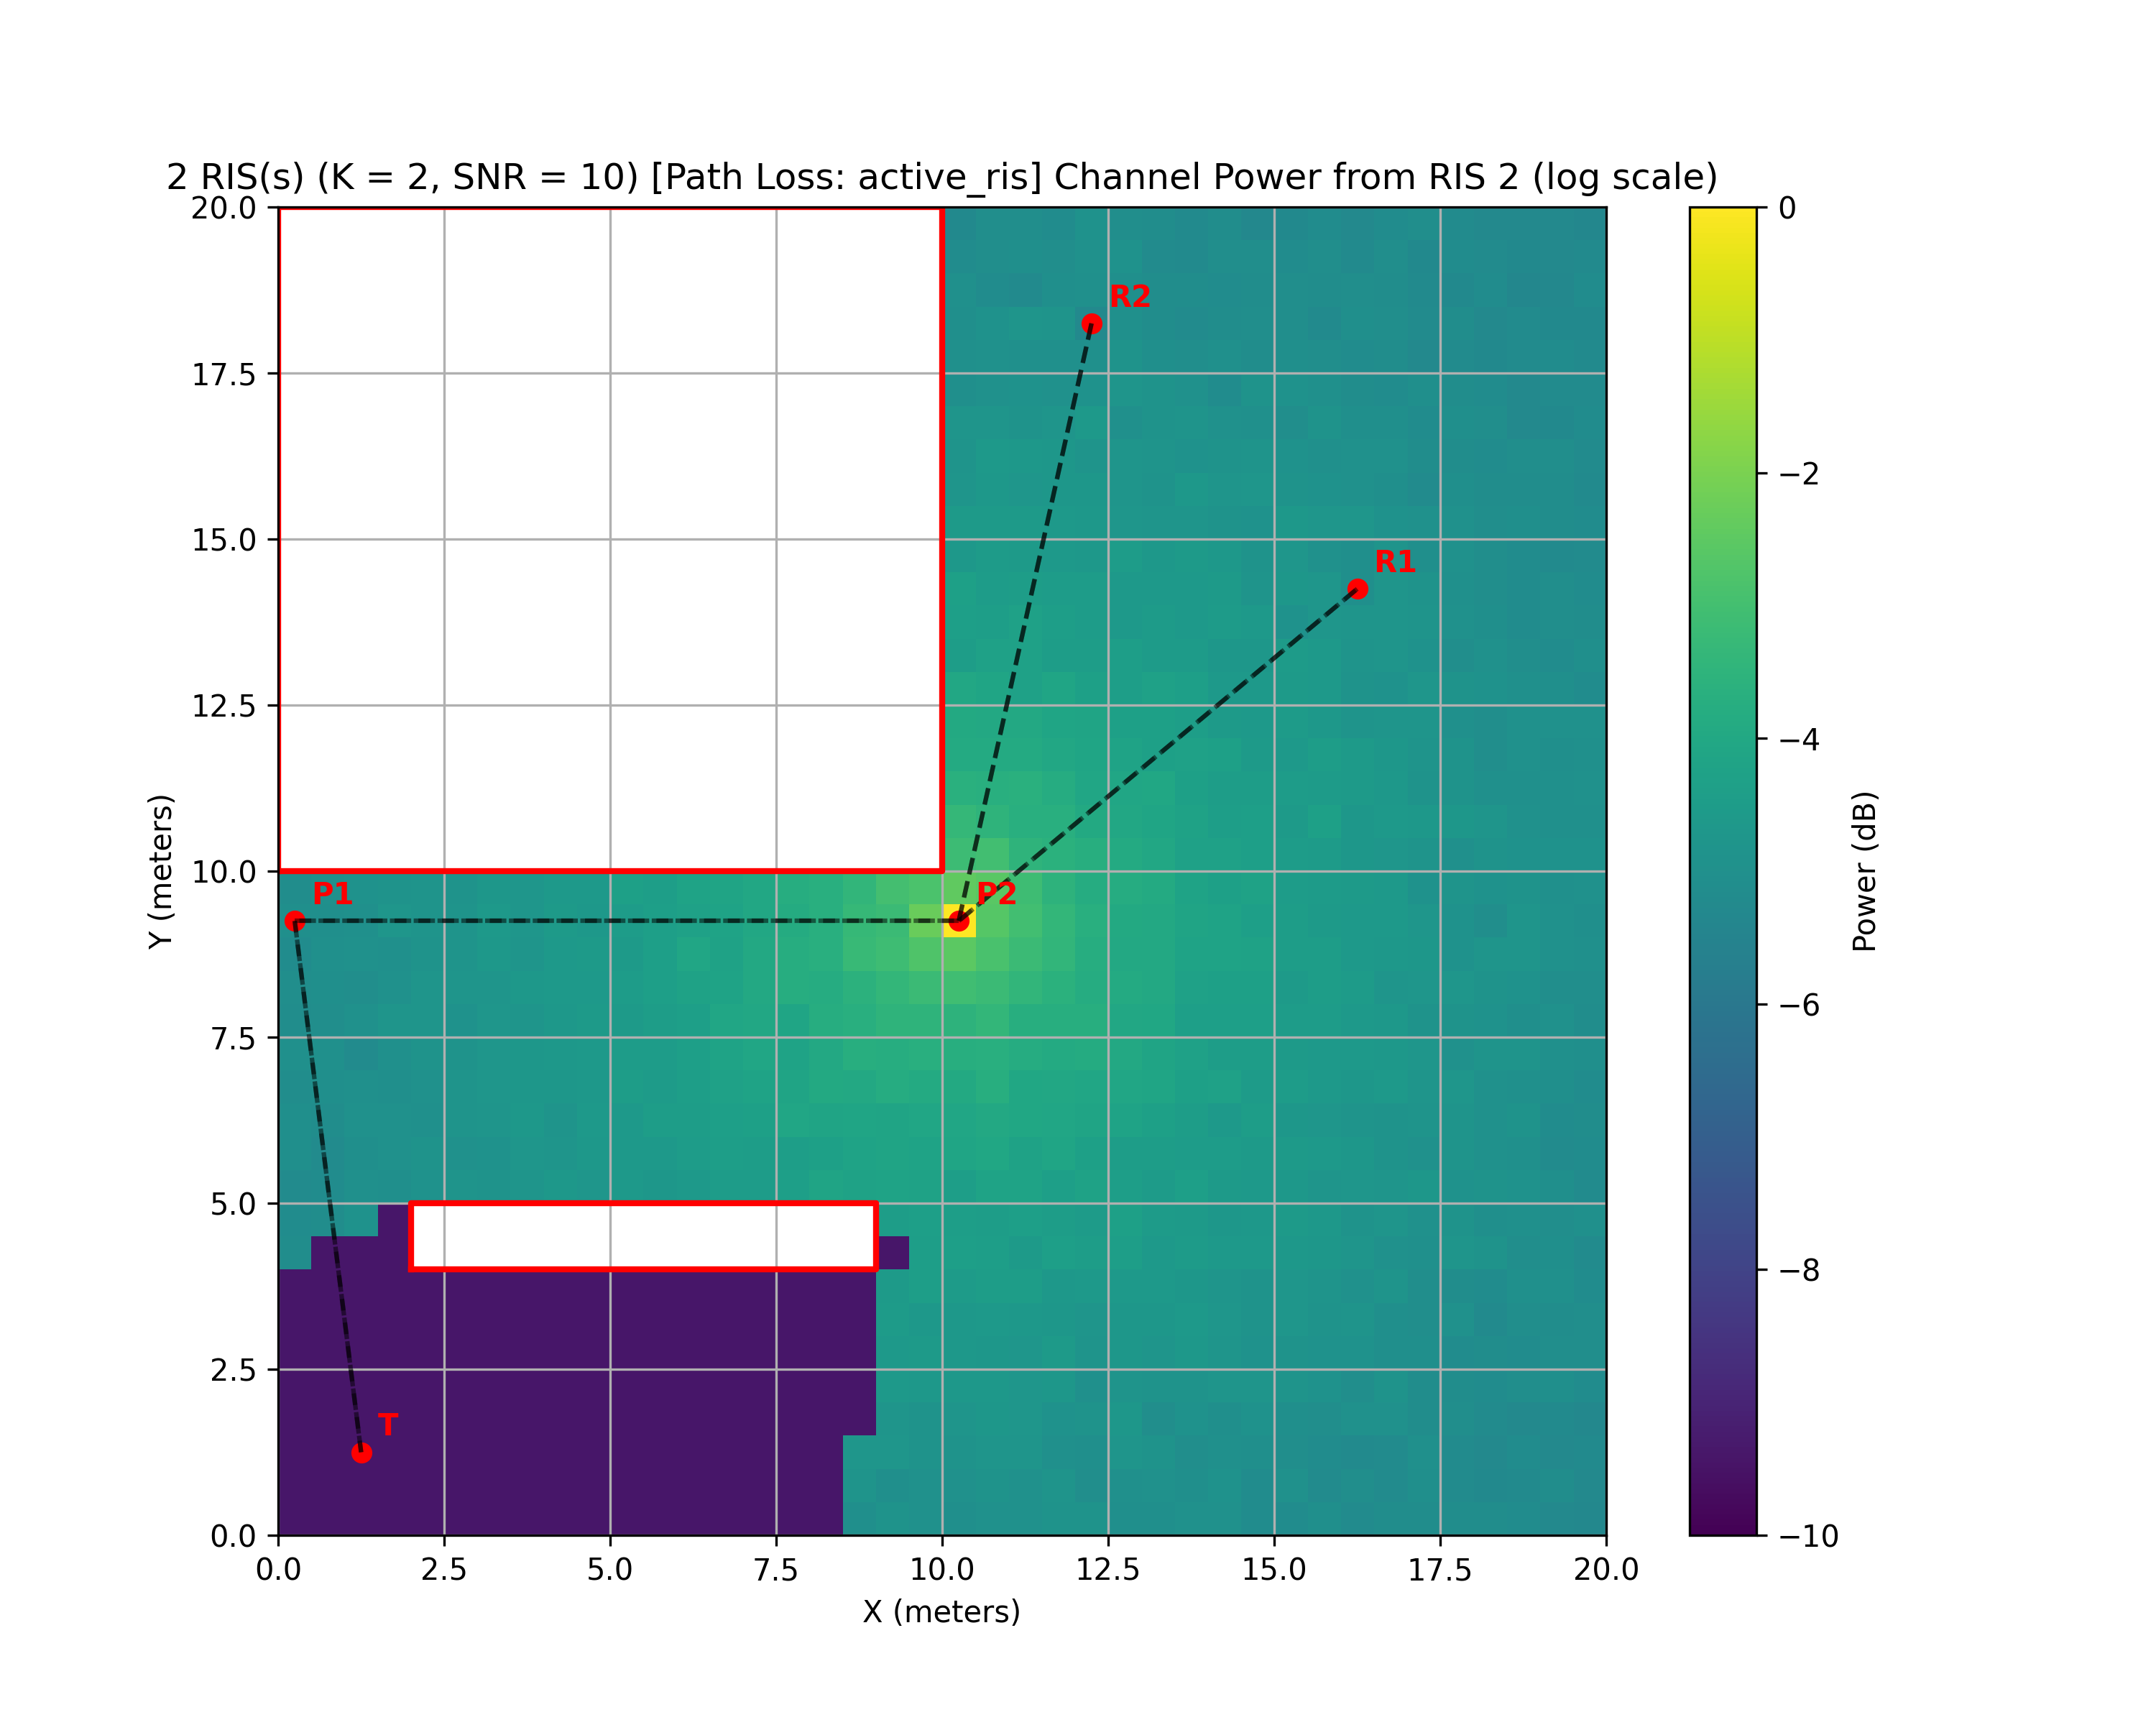
\includegraphics[width=0.8\linewidth]{imgs/heatmap-simulations/2 RIS(s) (K = 2, SNR = 10) [Path Loss_ active_ris] Channel Power from RIS 2 (log scale).png}
%   \caption{2 RIS(s) (K = 2, SNR = 10) [Path Loss: active ris] Channel Power from RIS 2 (log scale)}
% \end{figure}

% \begin{figure}[H]
%   \centering
%   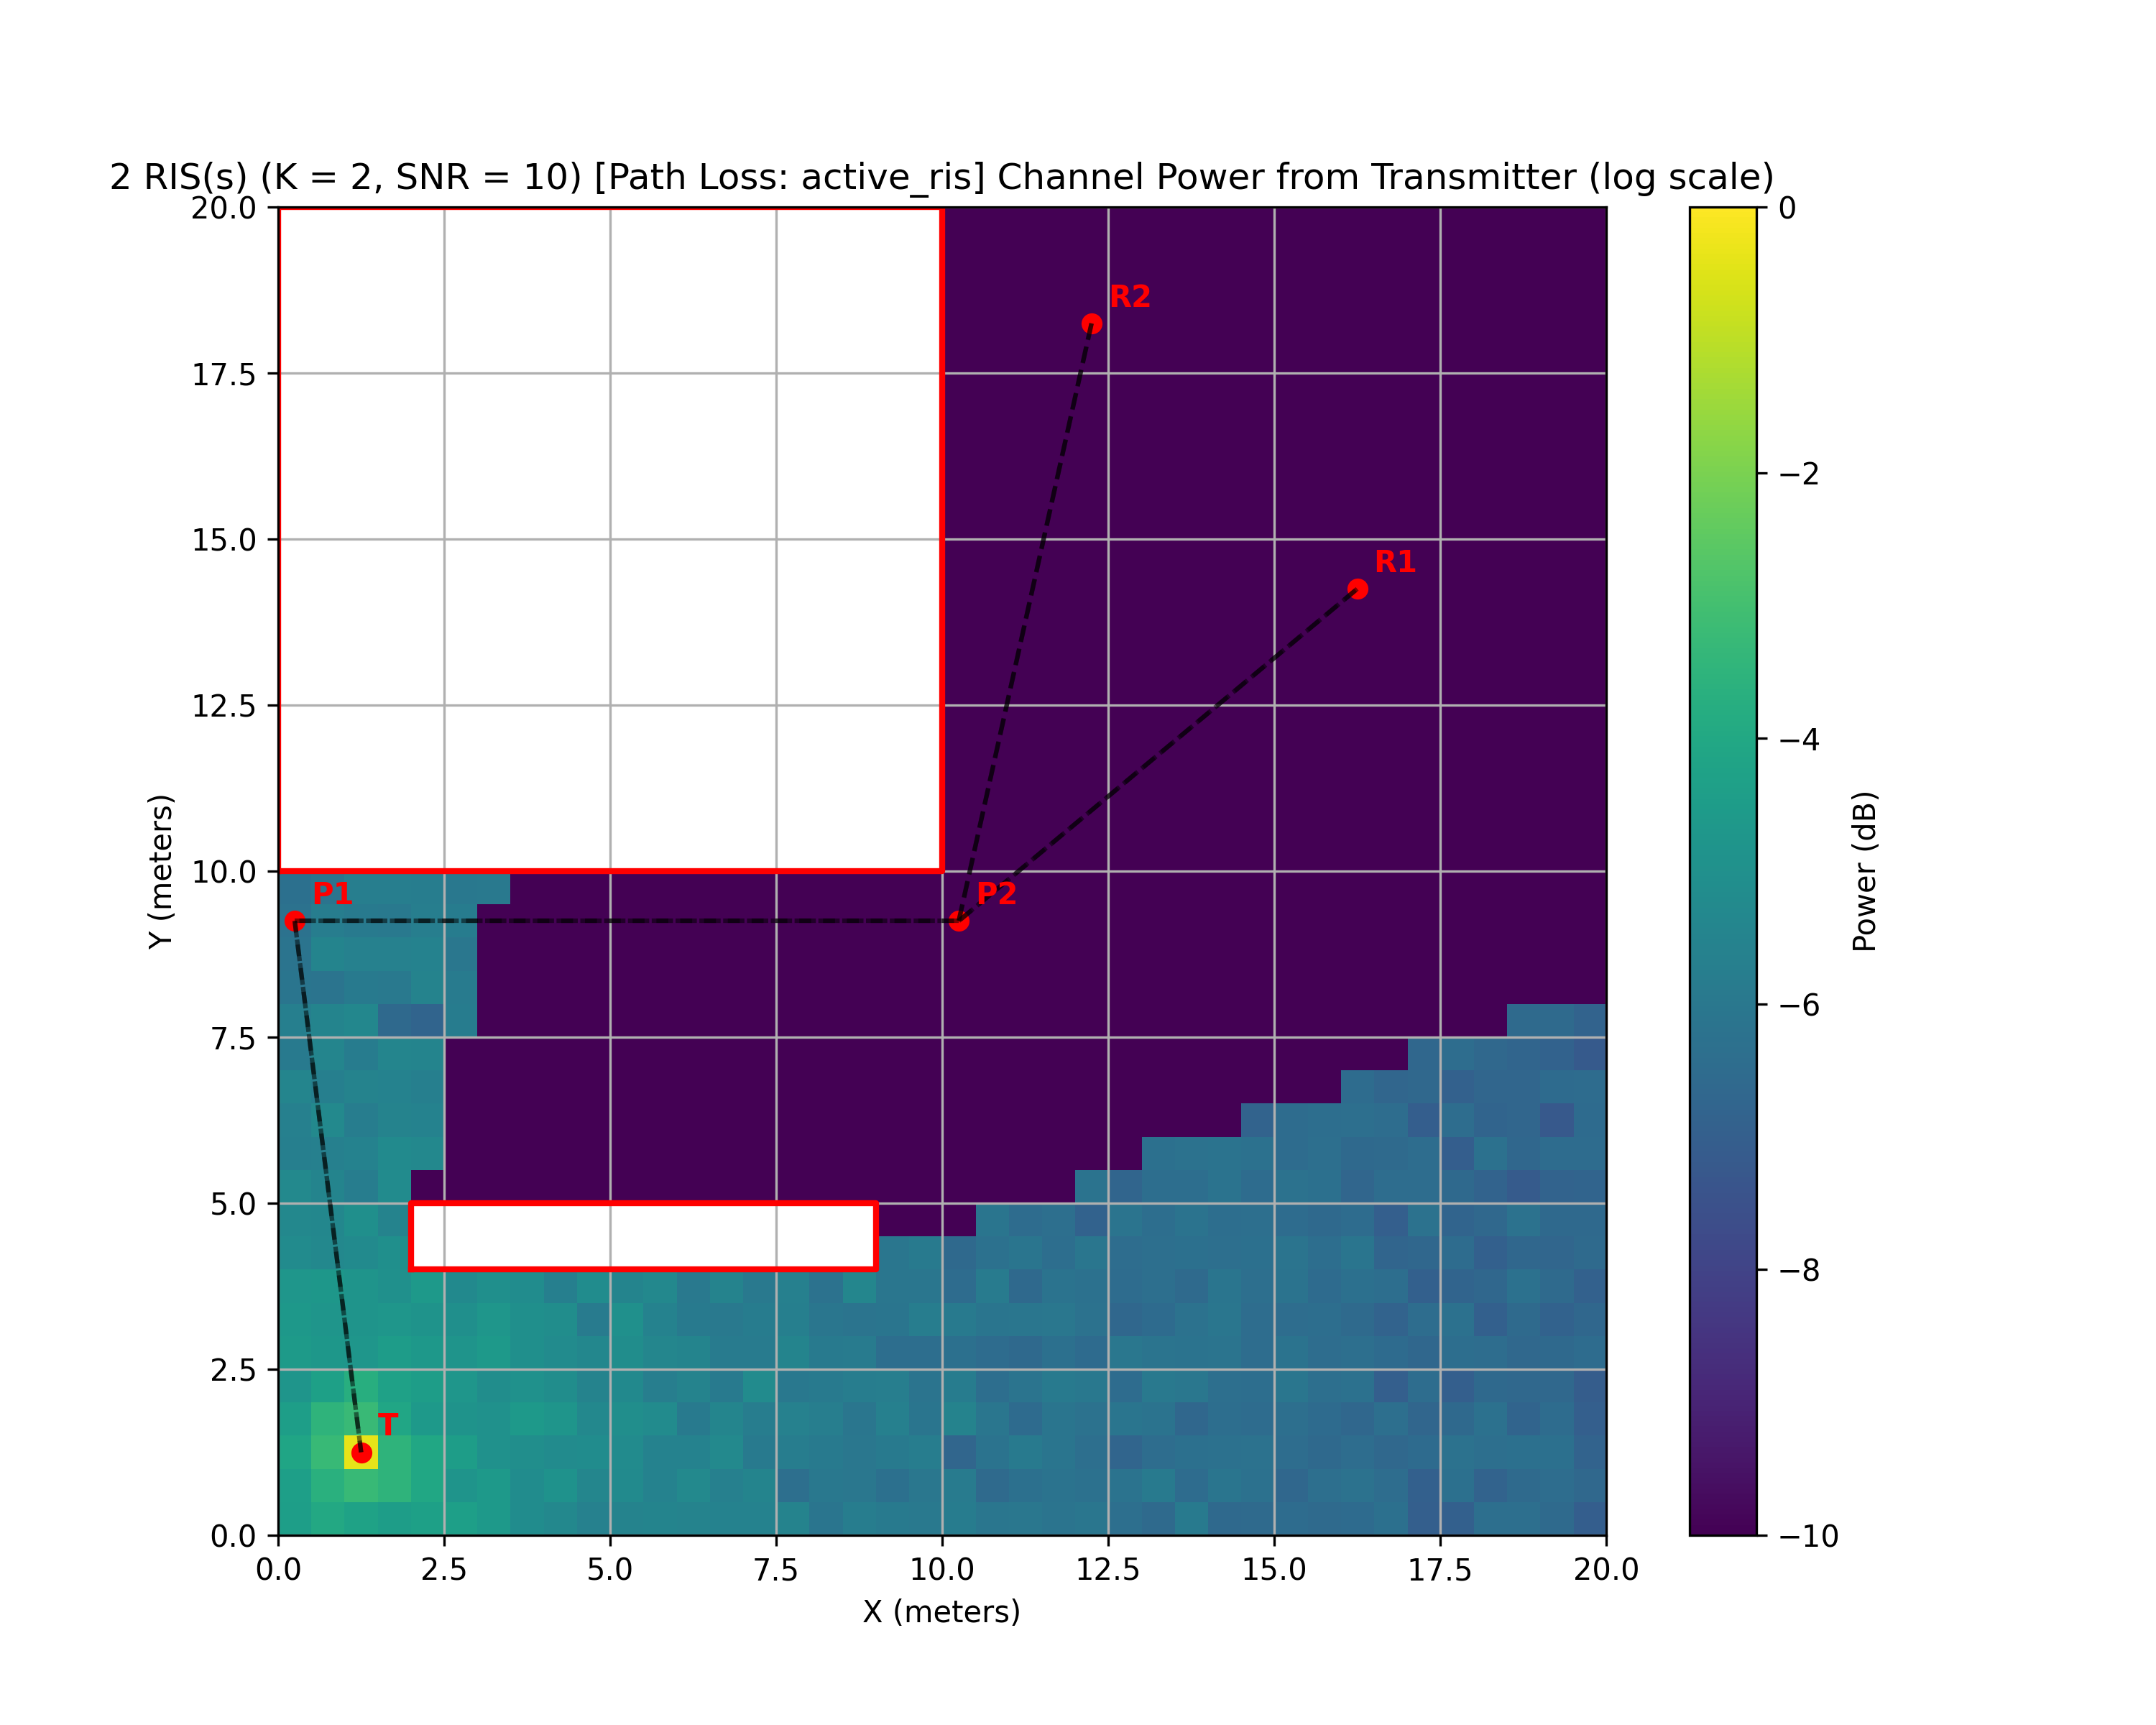
\includegraphics[width=0.8\linewidth]{imgs/heatmap-simulations/2 RIS(s) (K = 2, SNR = 10) [Path Loss_ active_ris] Channel Power from Transmitter (log scale).png}
%   \caption{2 RIS(s) (K = 2, SNR = 10) [Path Loss: active ris] Channel Power from Transmitter (log scale)}
% \end{figure}

% \begin{figure}[H]
%   \centering
%   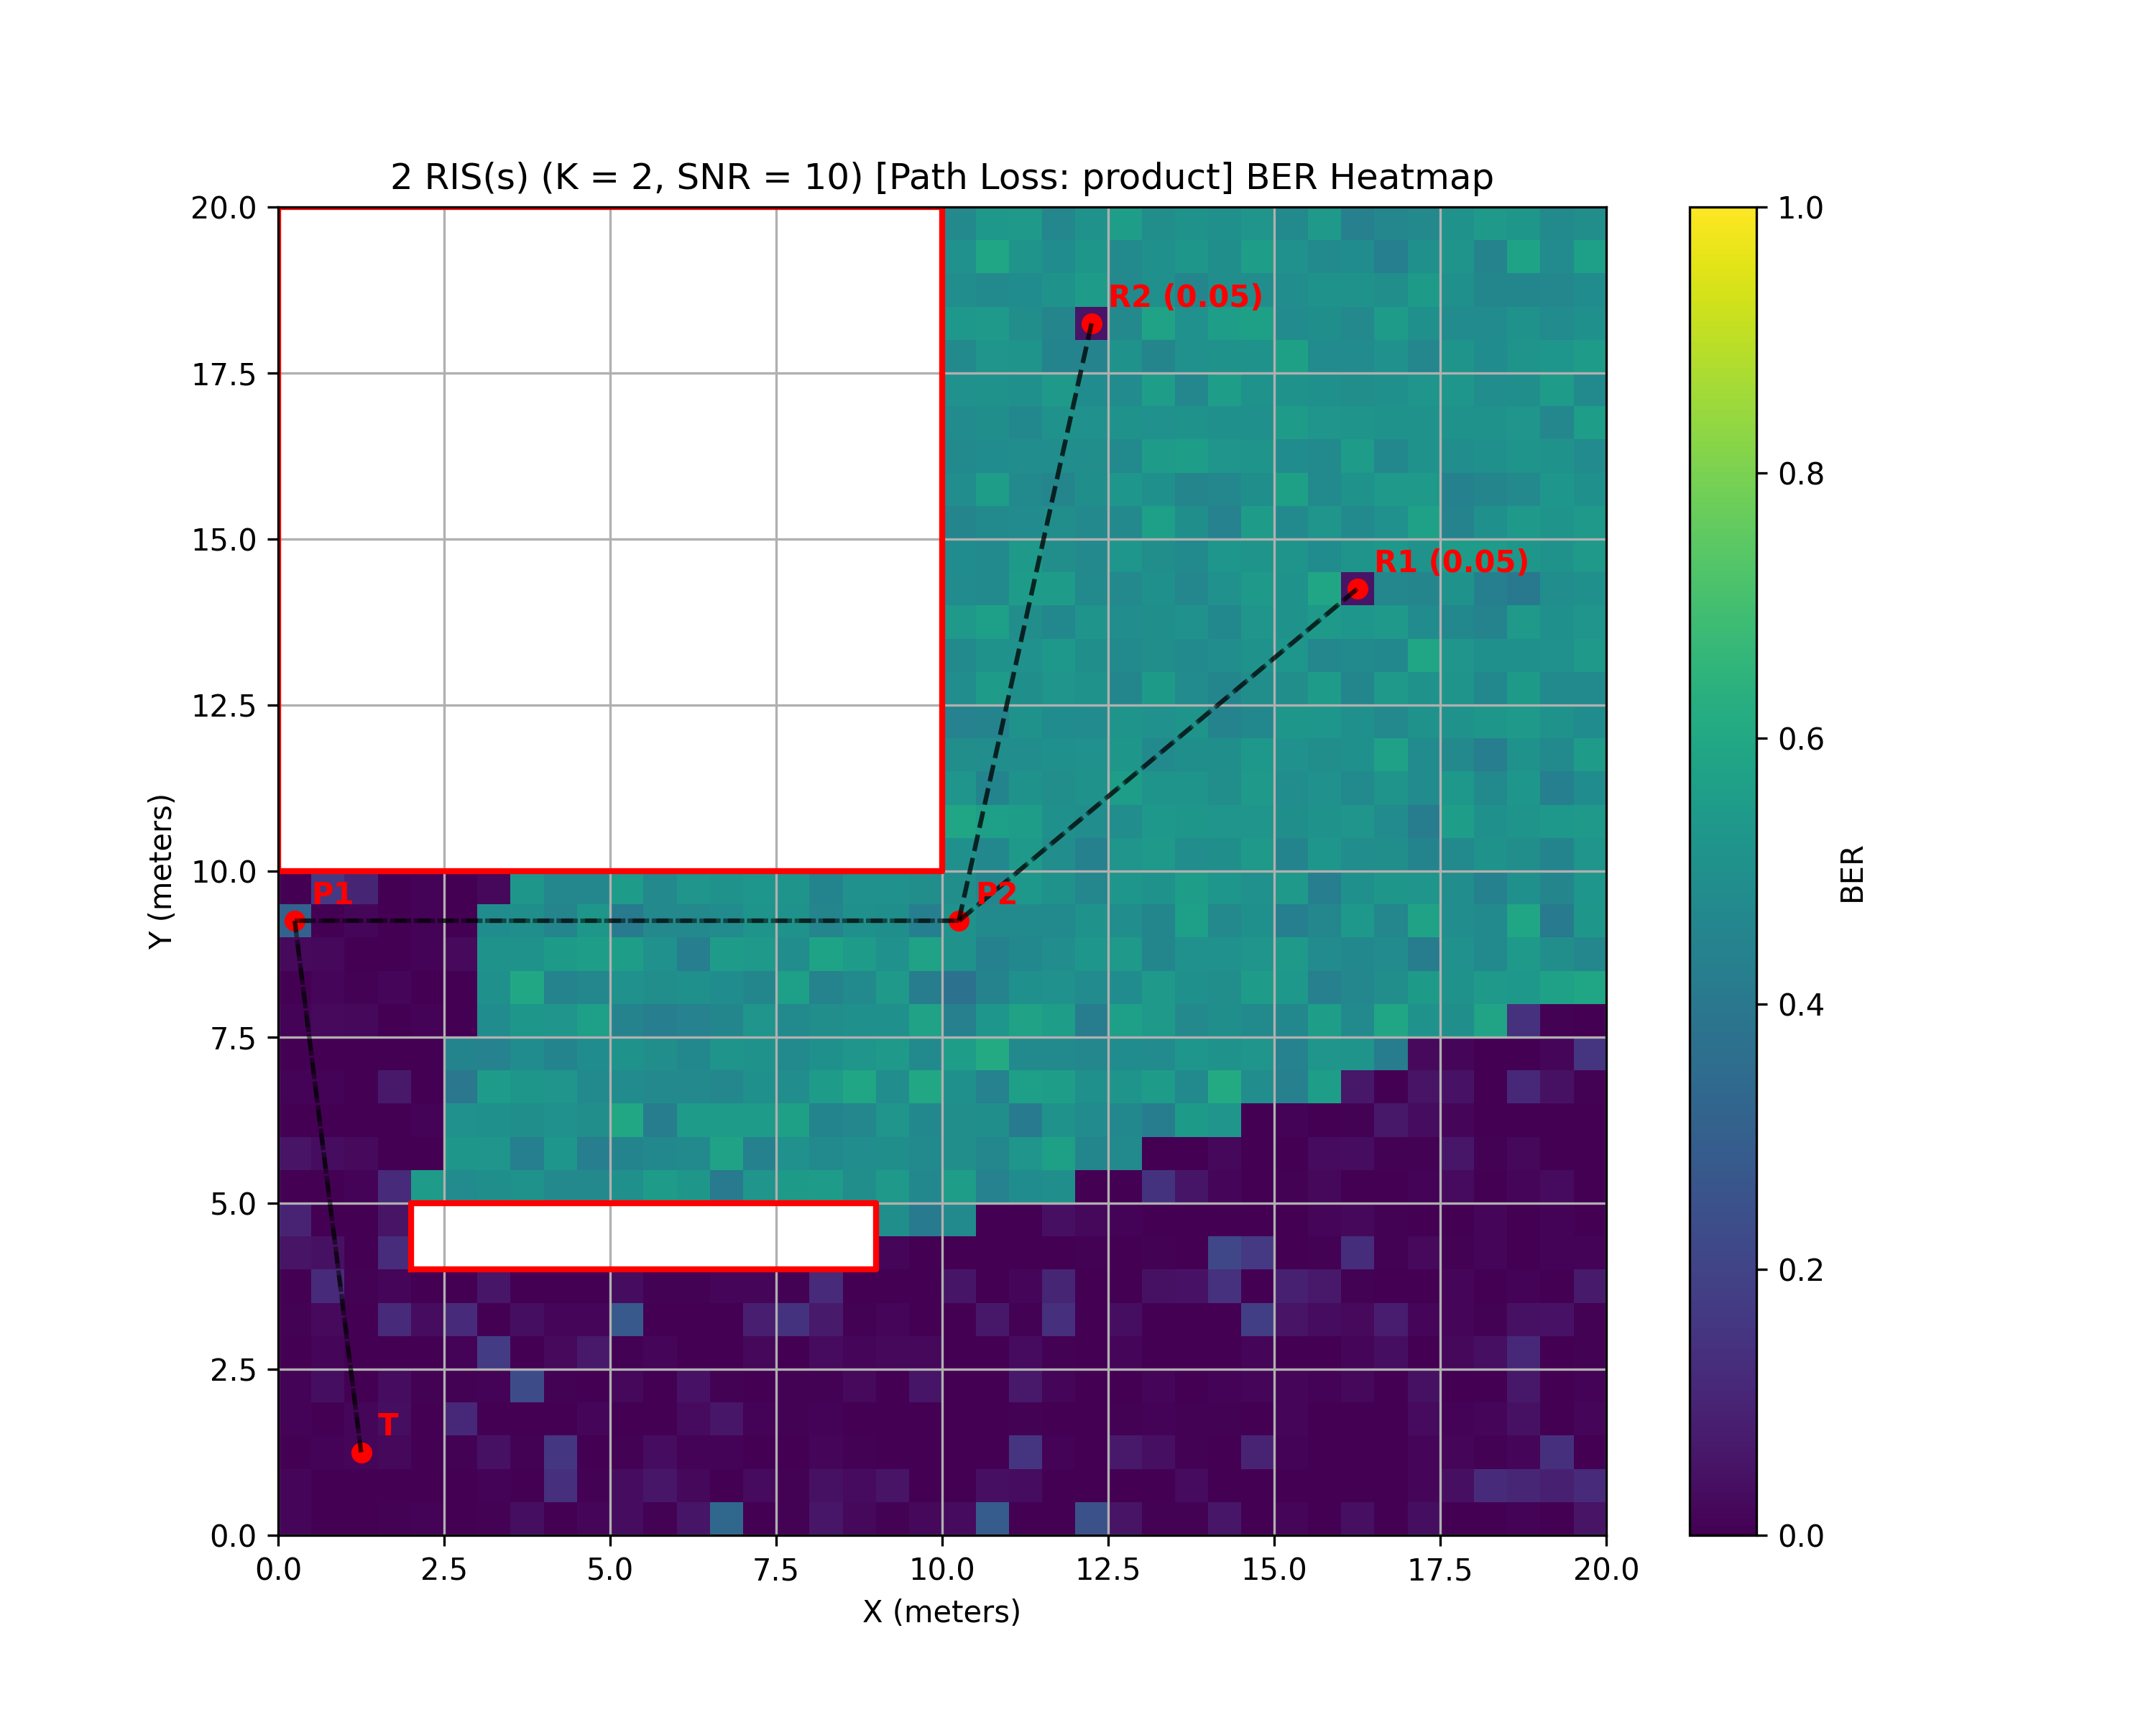
\includegraphics[width=0.8\linewidth]{imgs/heatmap-simulations/2 RIS(s) (K = 2, SNR = 10) [Path Loss_ product] BER Heatmap.png}
%   \caption{2 RIS(s) (K = 2, SNR = 10) [Path Loss: product] BER Heatmap}
% \end{figure}

% \begin{figure}[H]
%   \centering
%   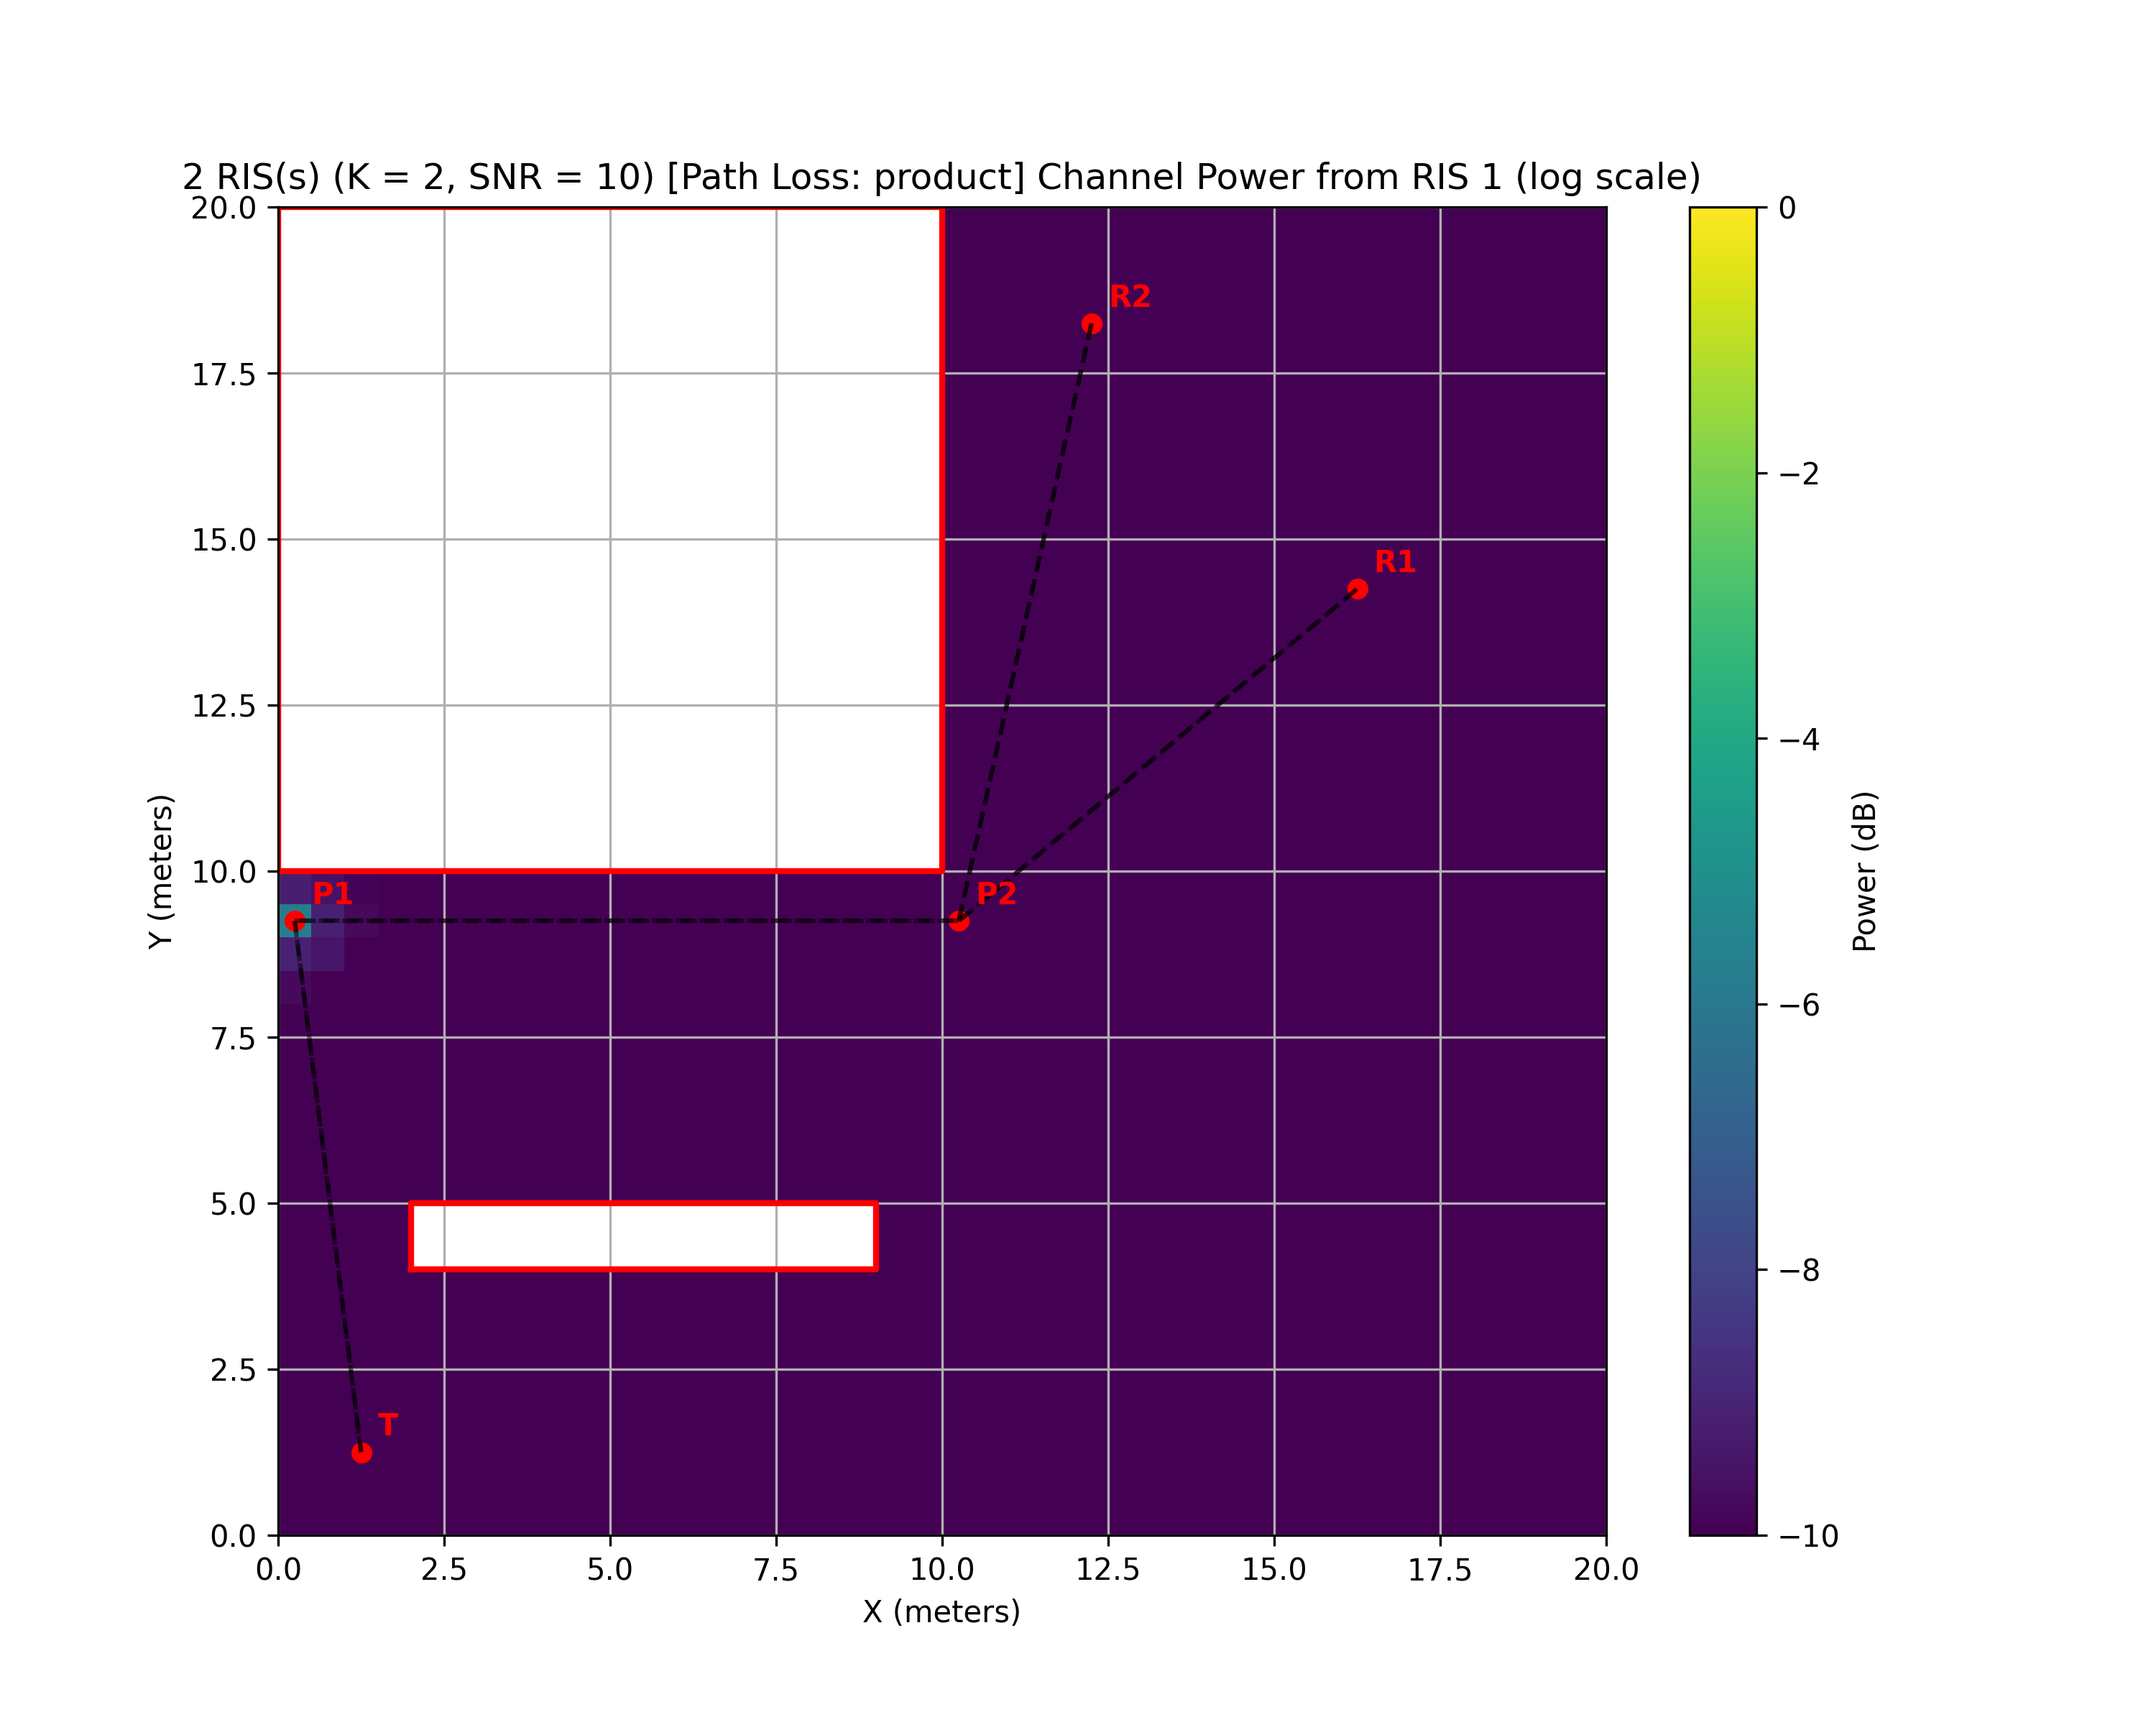
\includegraphics[width=0.8\linewidth]{imgs/heatmap-simulations/2 RIS(s) (K = 2, SNR = 10) [Path Loss_ product] Channel Power from RIS 1 (log scale).png}
%   \caption{2 RIS(s) (K = 2, SNR = 10) [Path Loss: product] Channel Power from RIS 1 (log scale)}
% \end{figure}

% \begin{figure}[H]
%   \centering
%   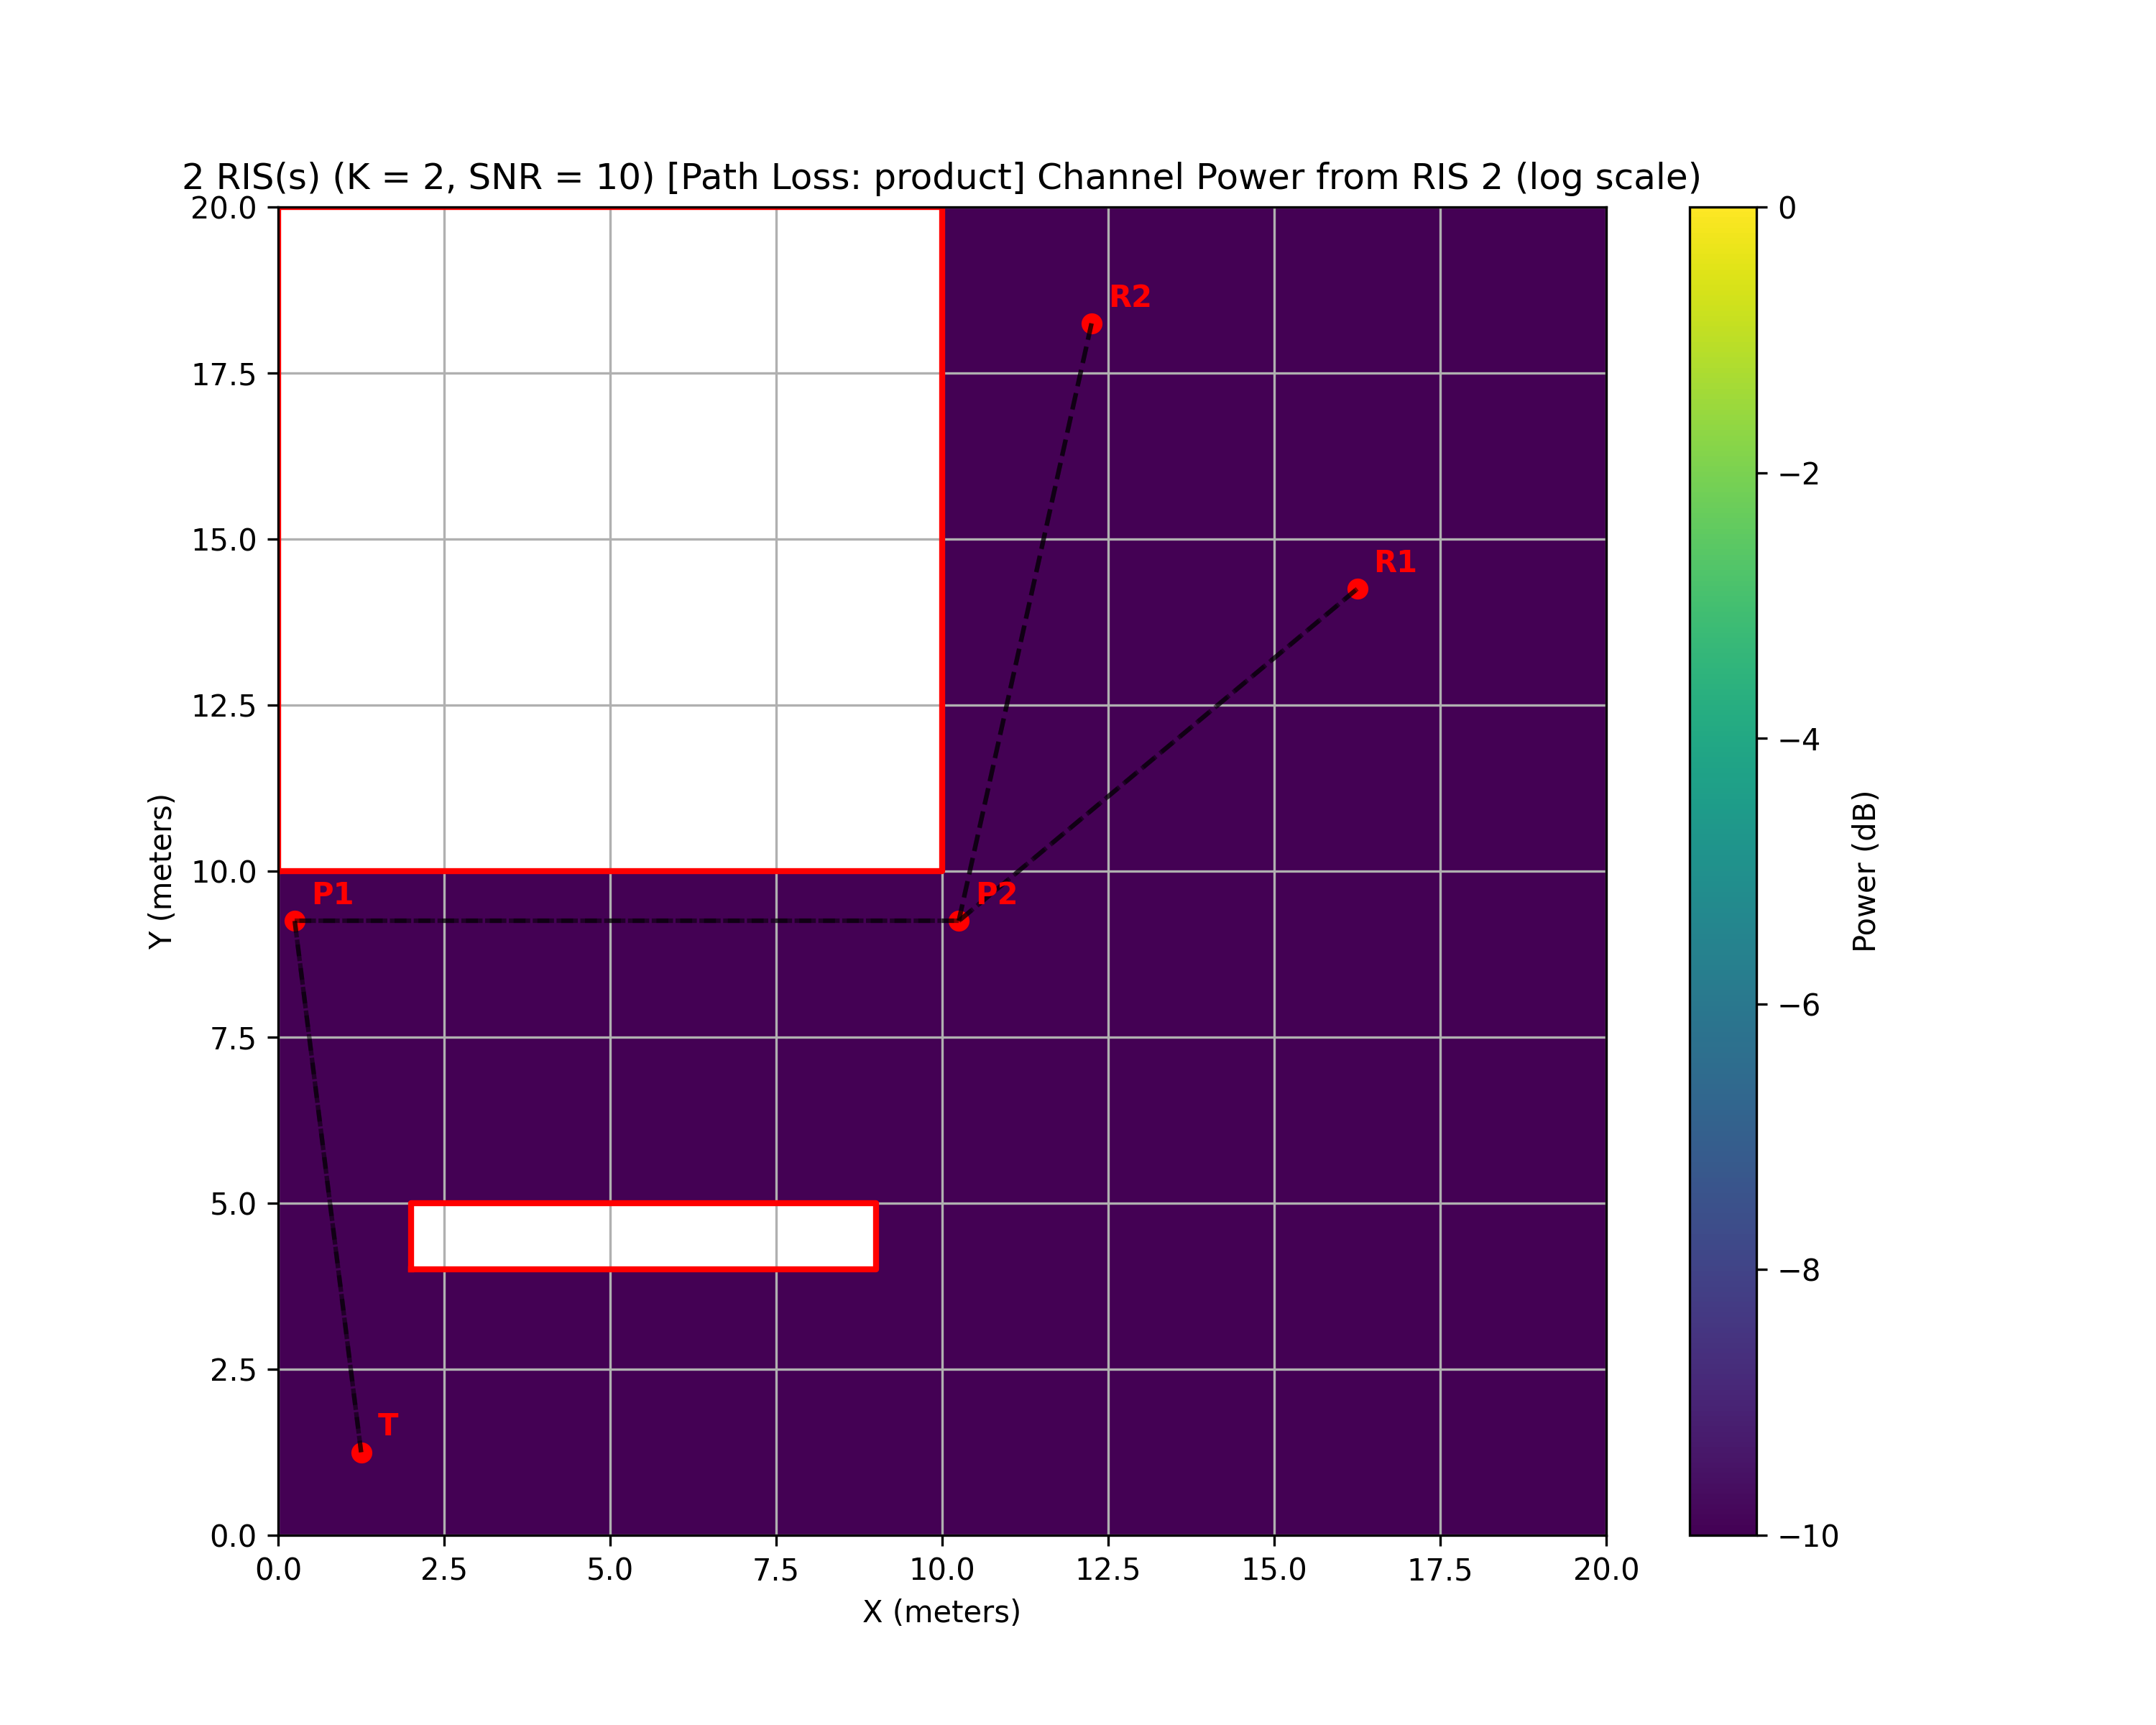
\includegraphics[width=0.8\linewidth]{imgs/heatmap-simulations/2 RIS(s) (K = 2, SNR = 10) [Path Loss_ product] Channel Power from RIS 2 (log scale).png}
%   \caption{2 RIS(s) (K = 2, SNR = 10) [Path Loss: product] Channel Power from RIS 2 (log scale)}
% \end{figure}

% \begin{figure}[H]
%   \centering
%   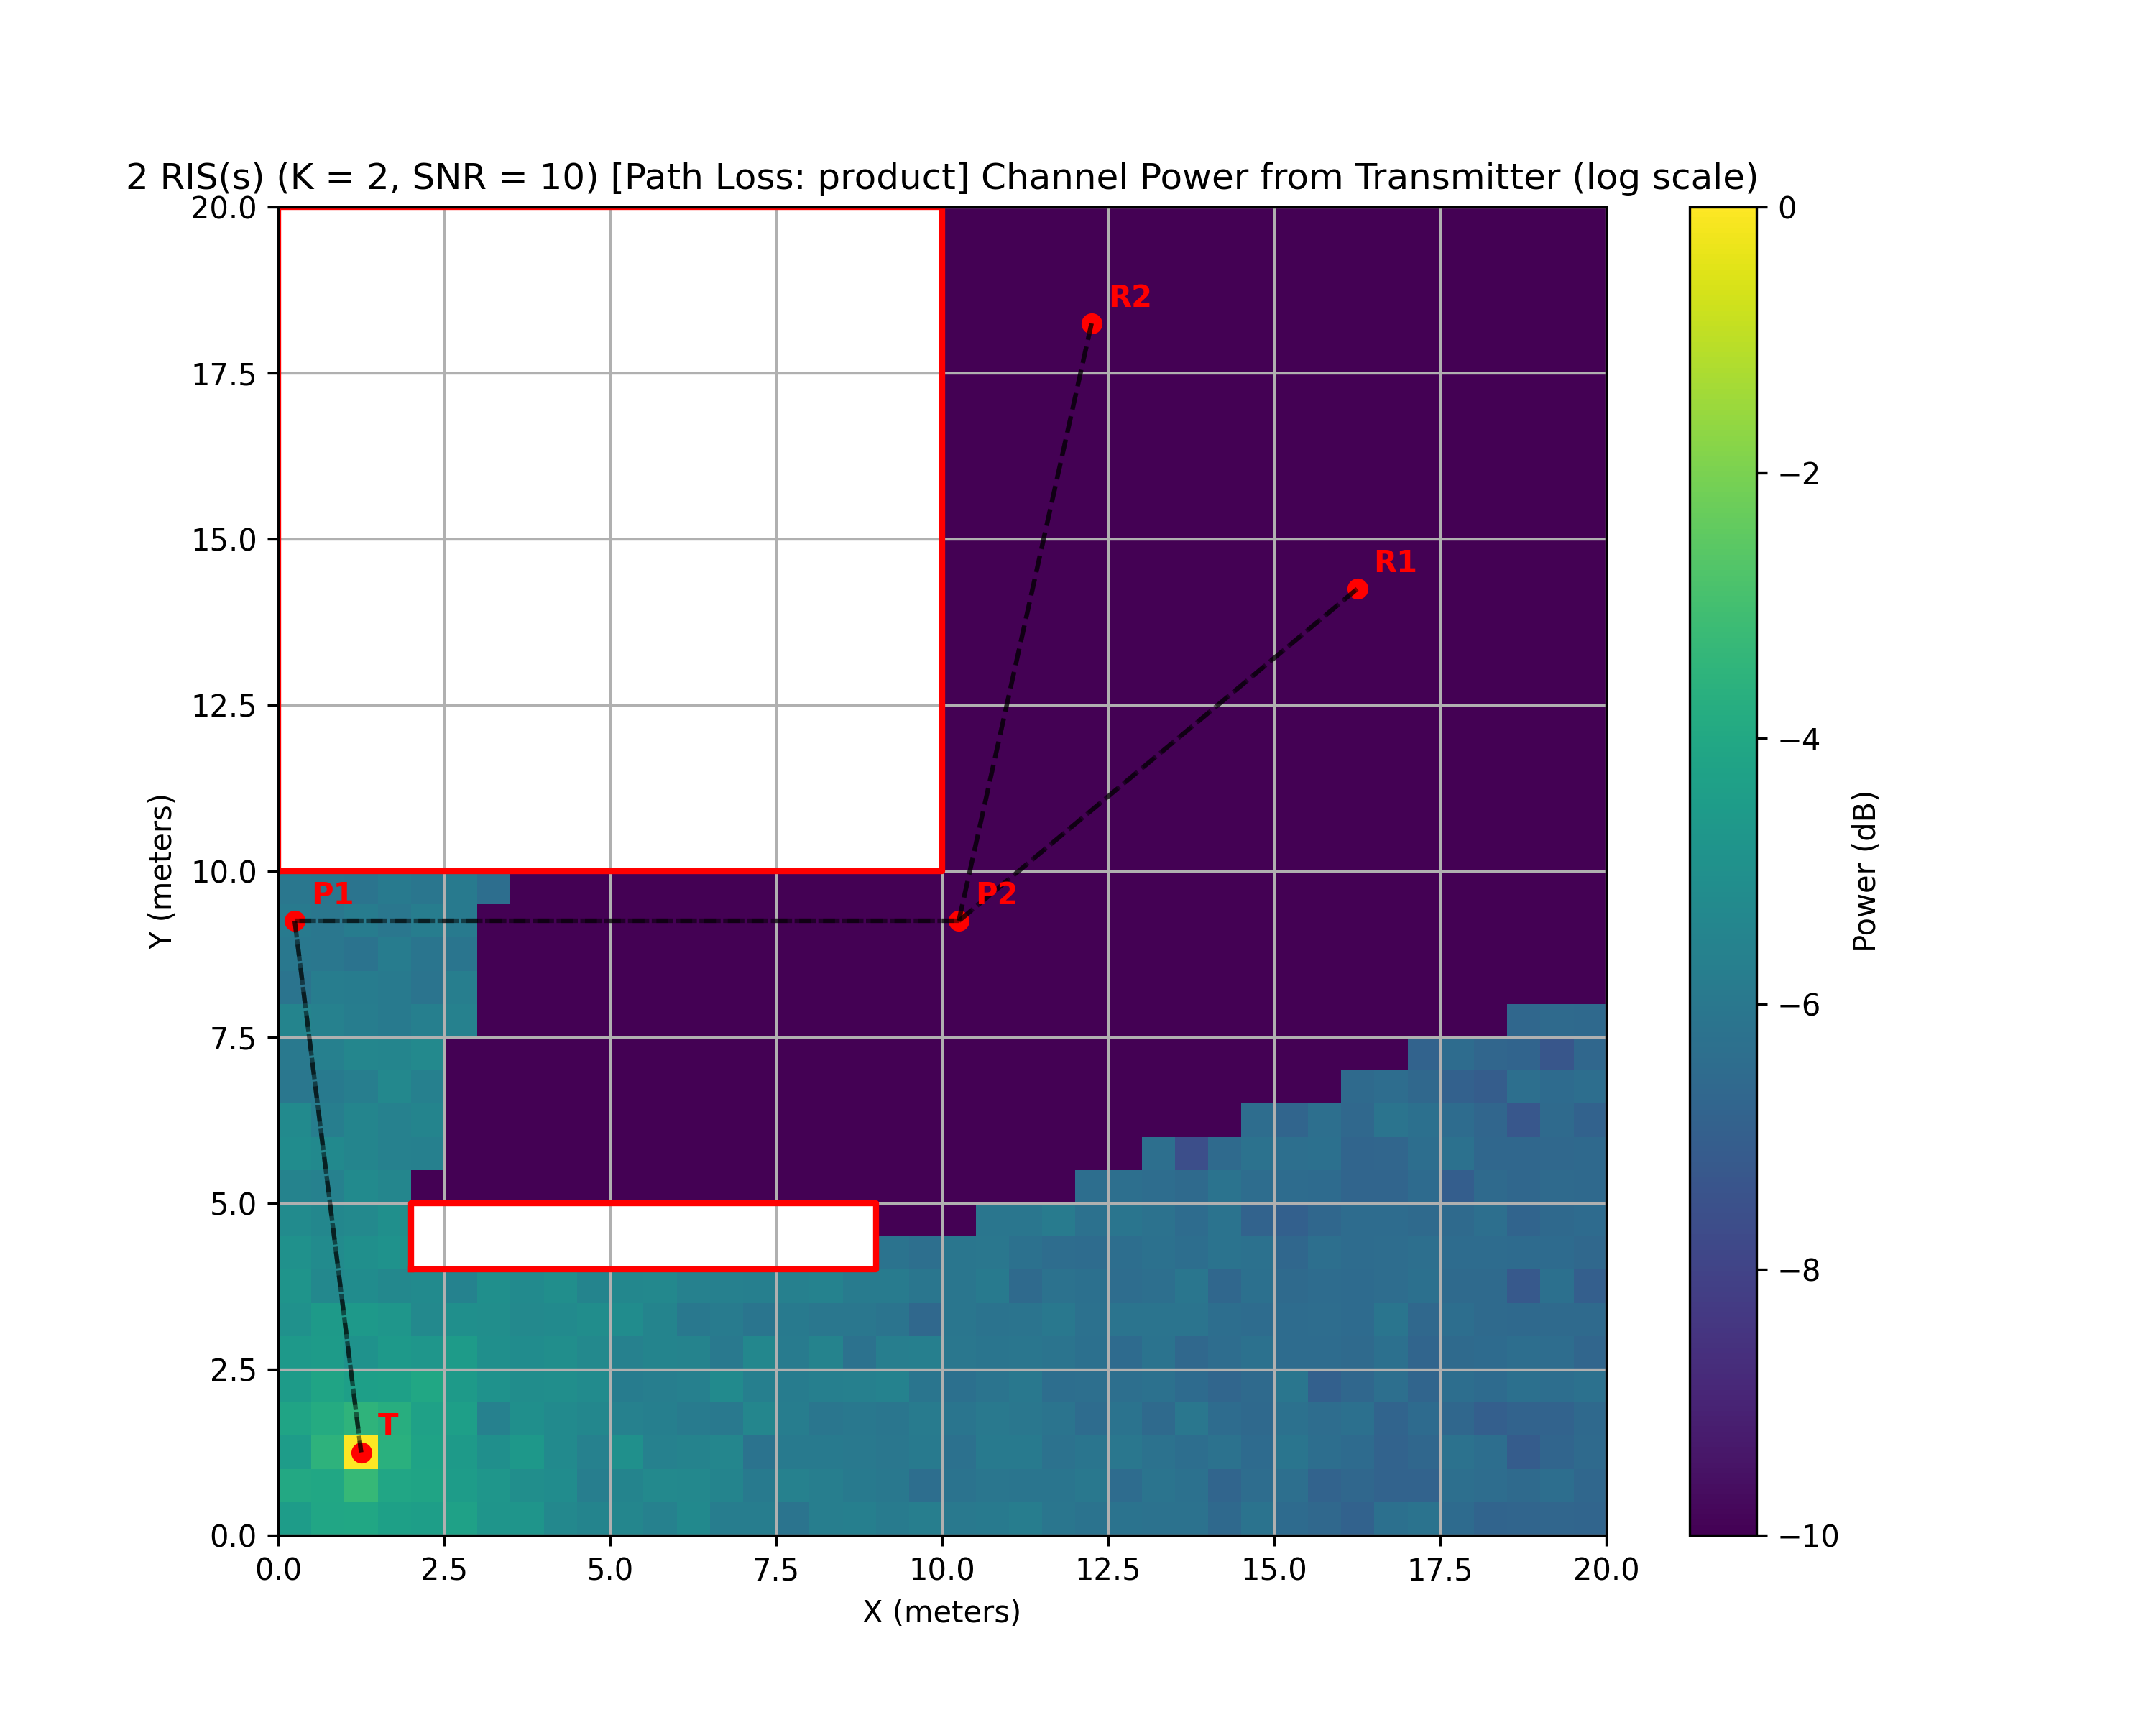
\includegraphics[width=0.8\linewidth]{imgs/heatmap-simulations/2 RIS(s) (K = 2, SNR = 10) [Path Loss_ product] Channel Power from Transmitter (log scale).png}
%   \caption{2 RIS(s) (K = 2, SNR = 10) [Path Loss: product] Channel Power from Transmitter (log scale)}
% \end{figure}

% \begin{figure}[H]
%   \centering
%   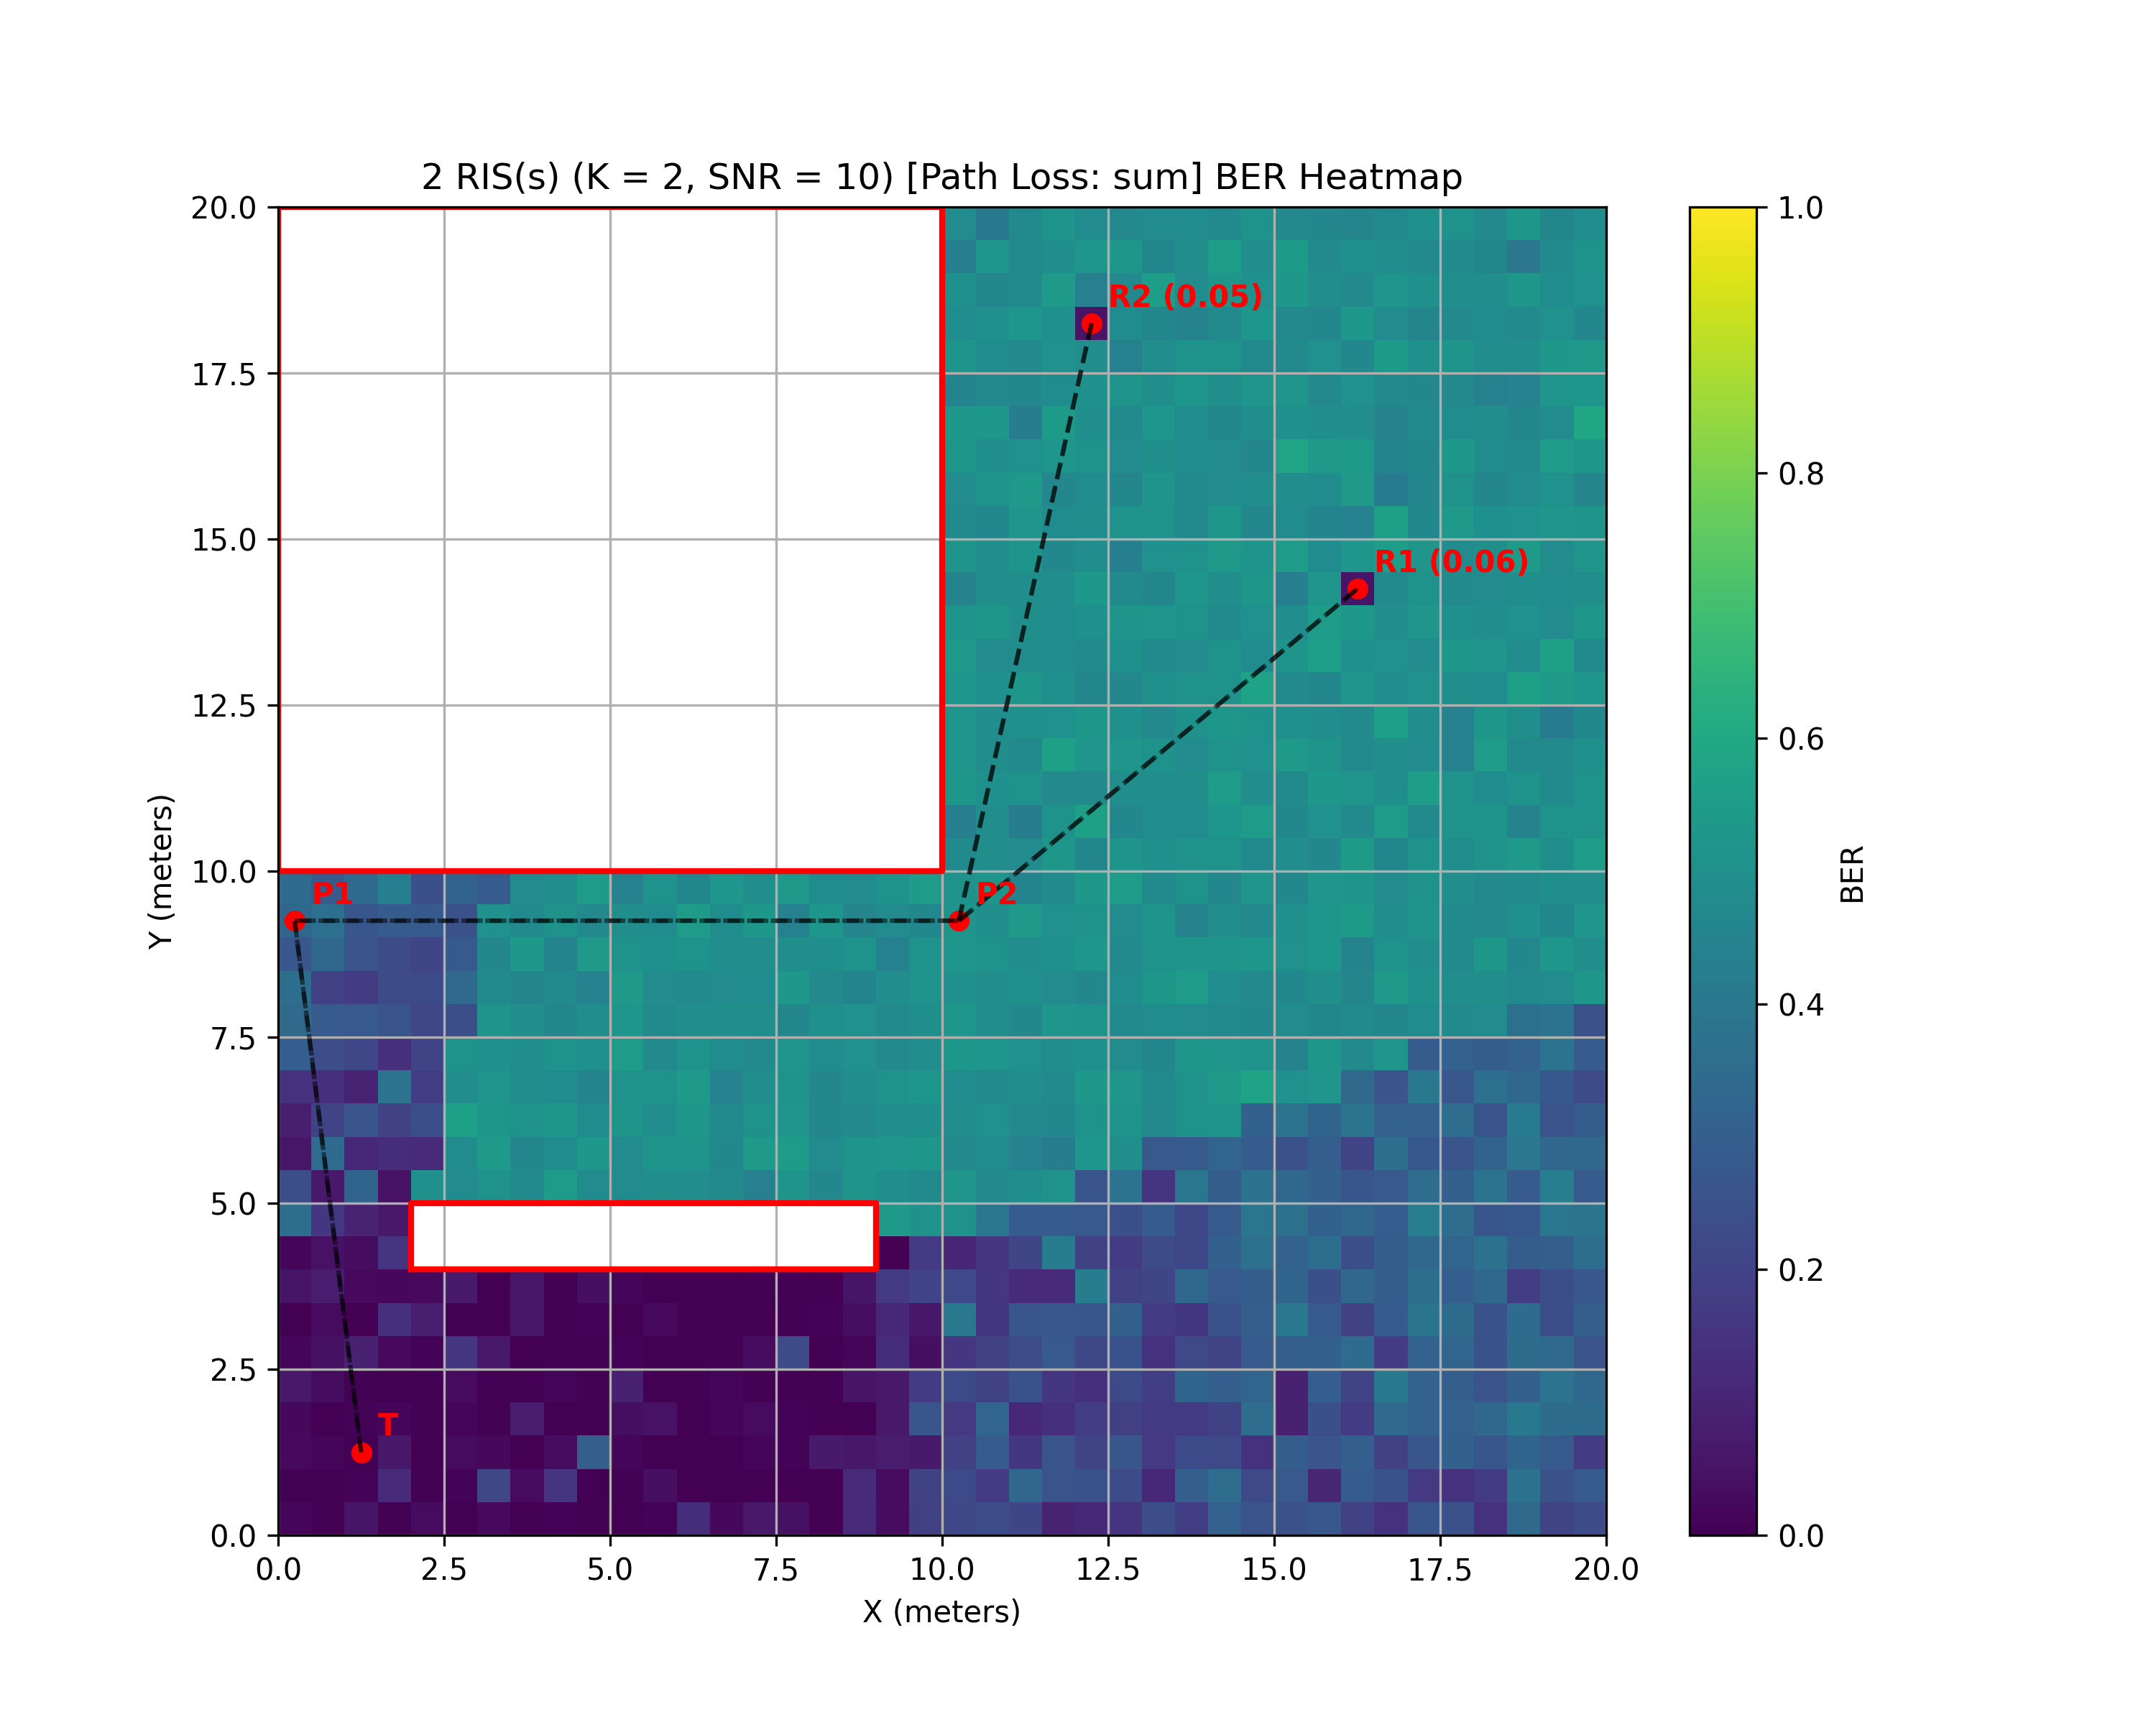
\includegraphics[width=0.8\linewidth]{imgs/heatmap-simulations/2 RIS(s) (K = 2, SNR = 10) [Path Loss_ sum] BER Heatmap.png}
%   \caption{2 RIS(s) (K = 2, SNR = 10) [Path Loss: sum] BER Heatmap}
% \end{figure}

% \begin{figure}[H]
%   \centering
%   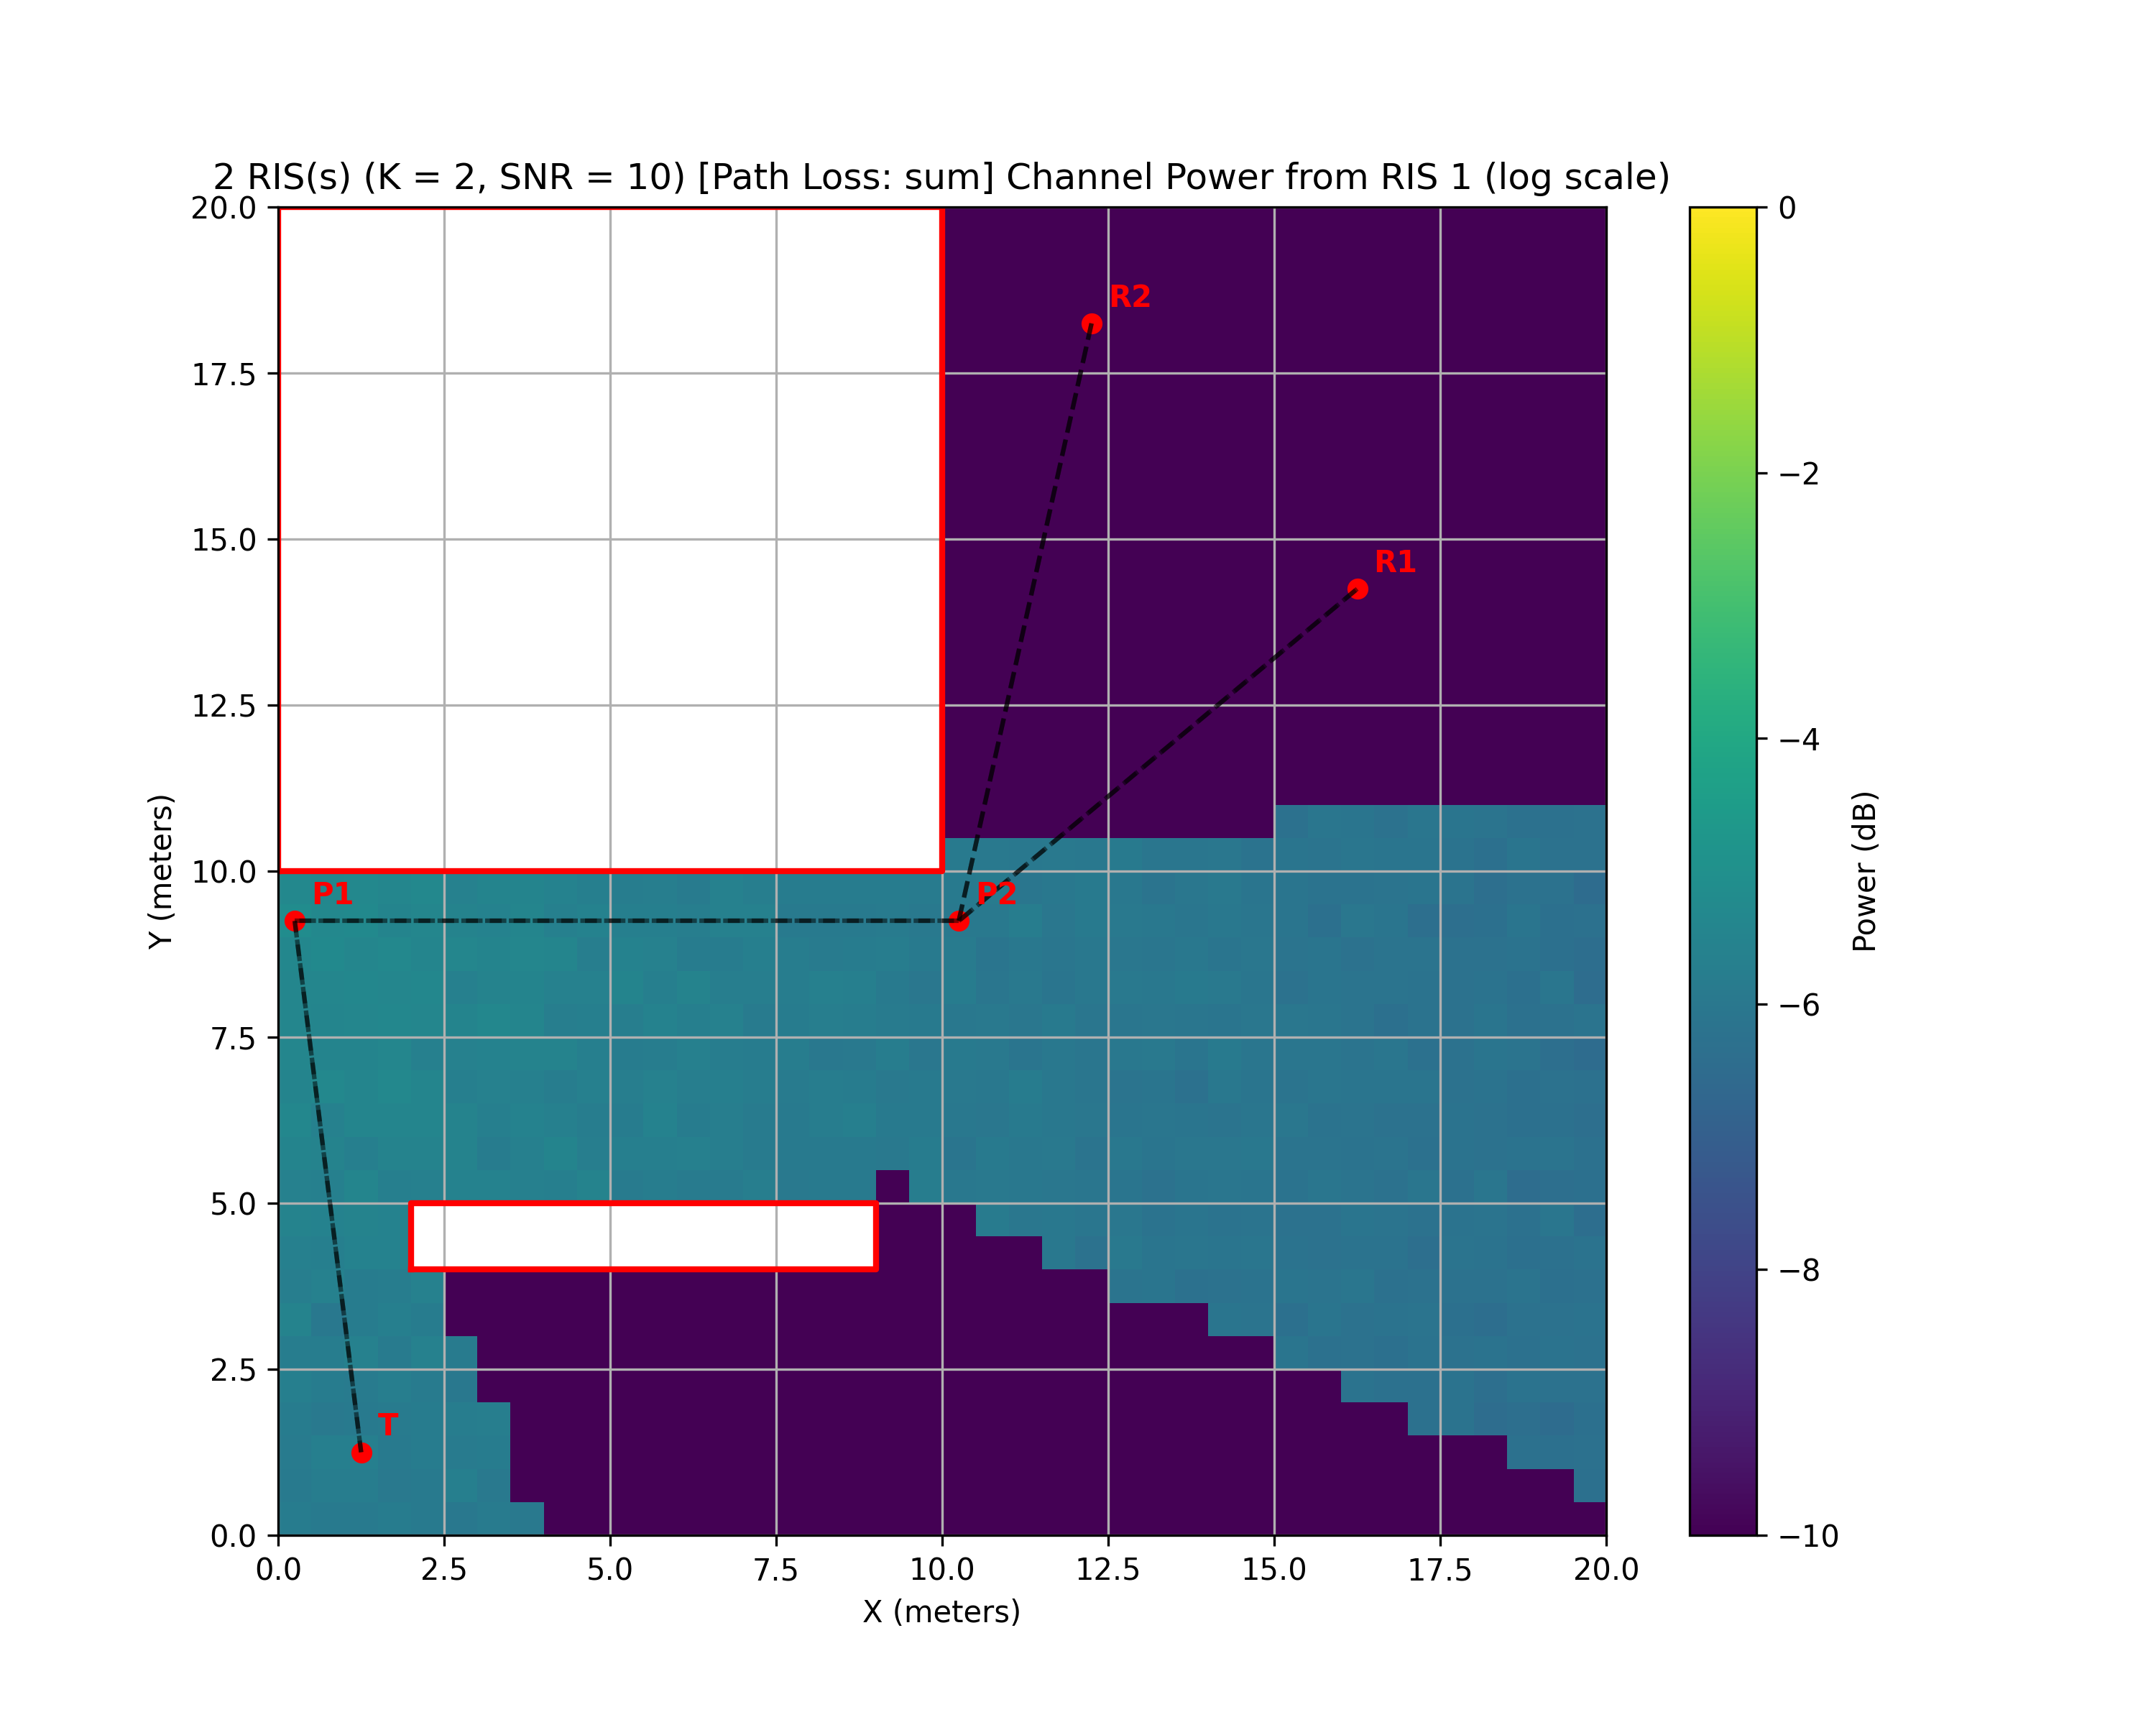
\includegraphics[width=0.8\linewidth]{imgs/heatmap-simulations/2 RIS(s) (K = 2, SNR = 10) [Path Loss_ sum] Channel Power from RIS 1 (log scale).png}
%   \caption{2 RIS(s) (K = 2, SNR = 10) [Path Loss: sum] Channel Power from RIS 1 (log scale)}
% \end{figure}

% \begin{figure}[H]
%   \centering
%   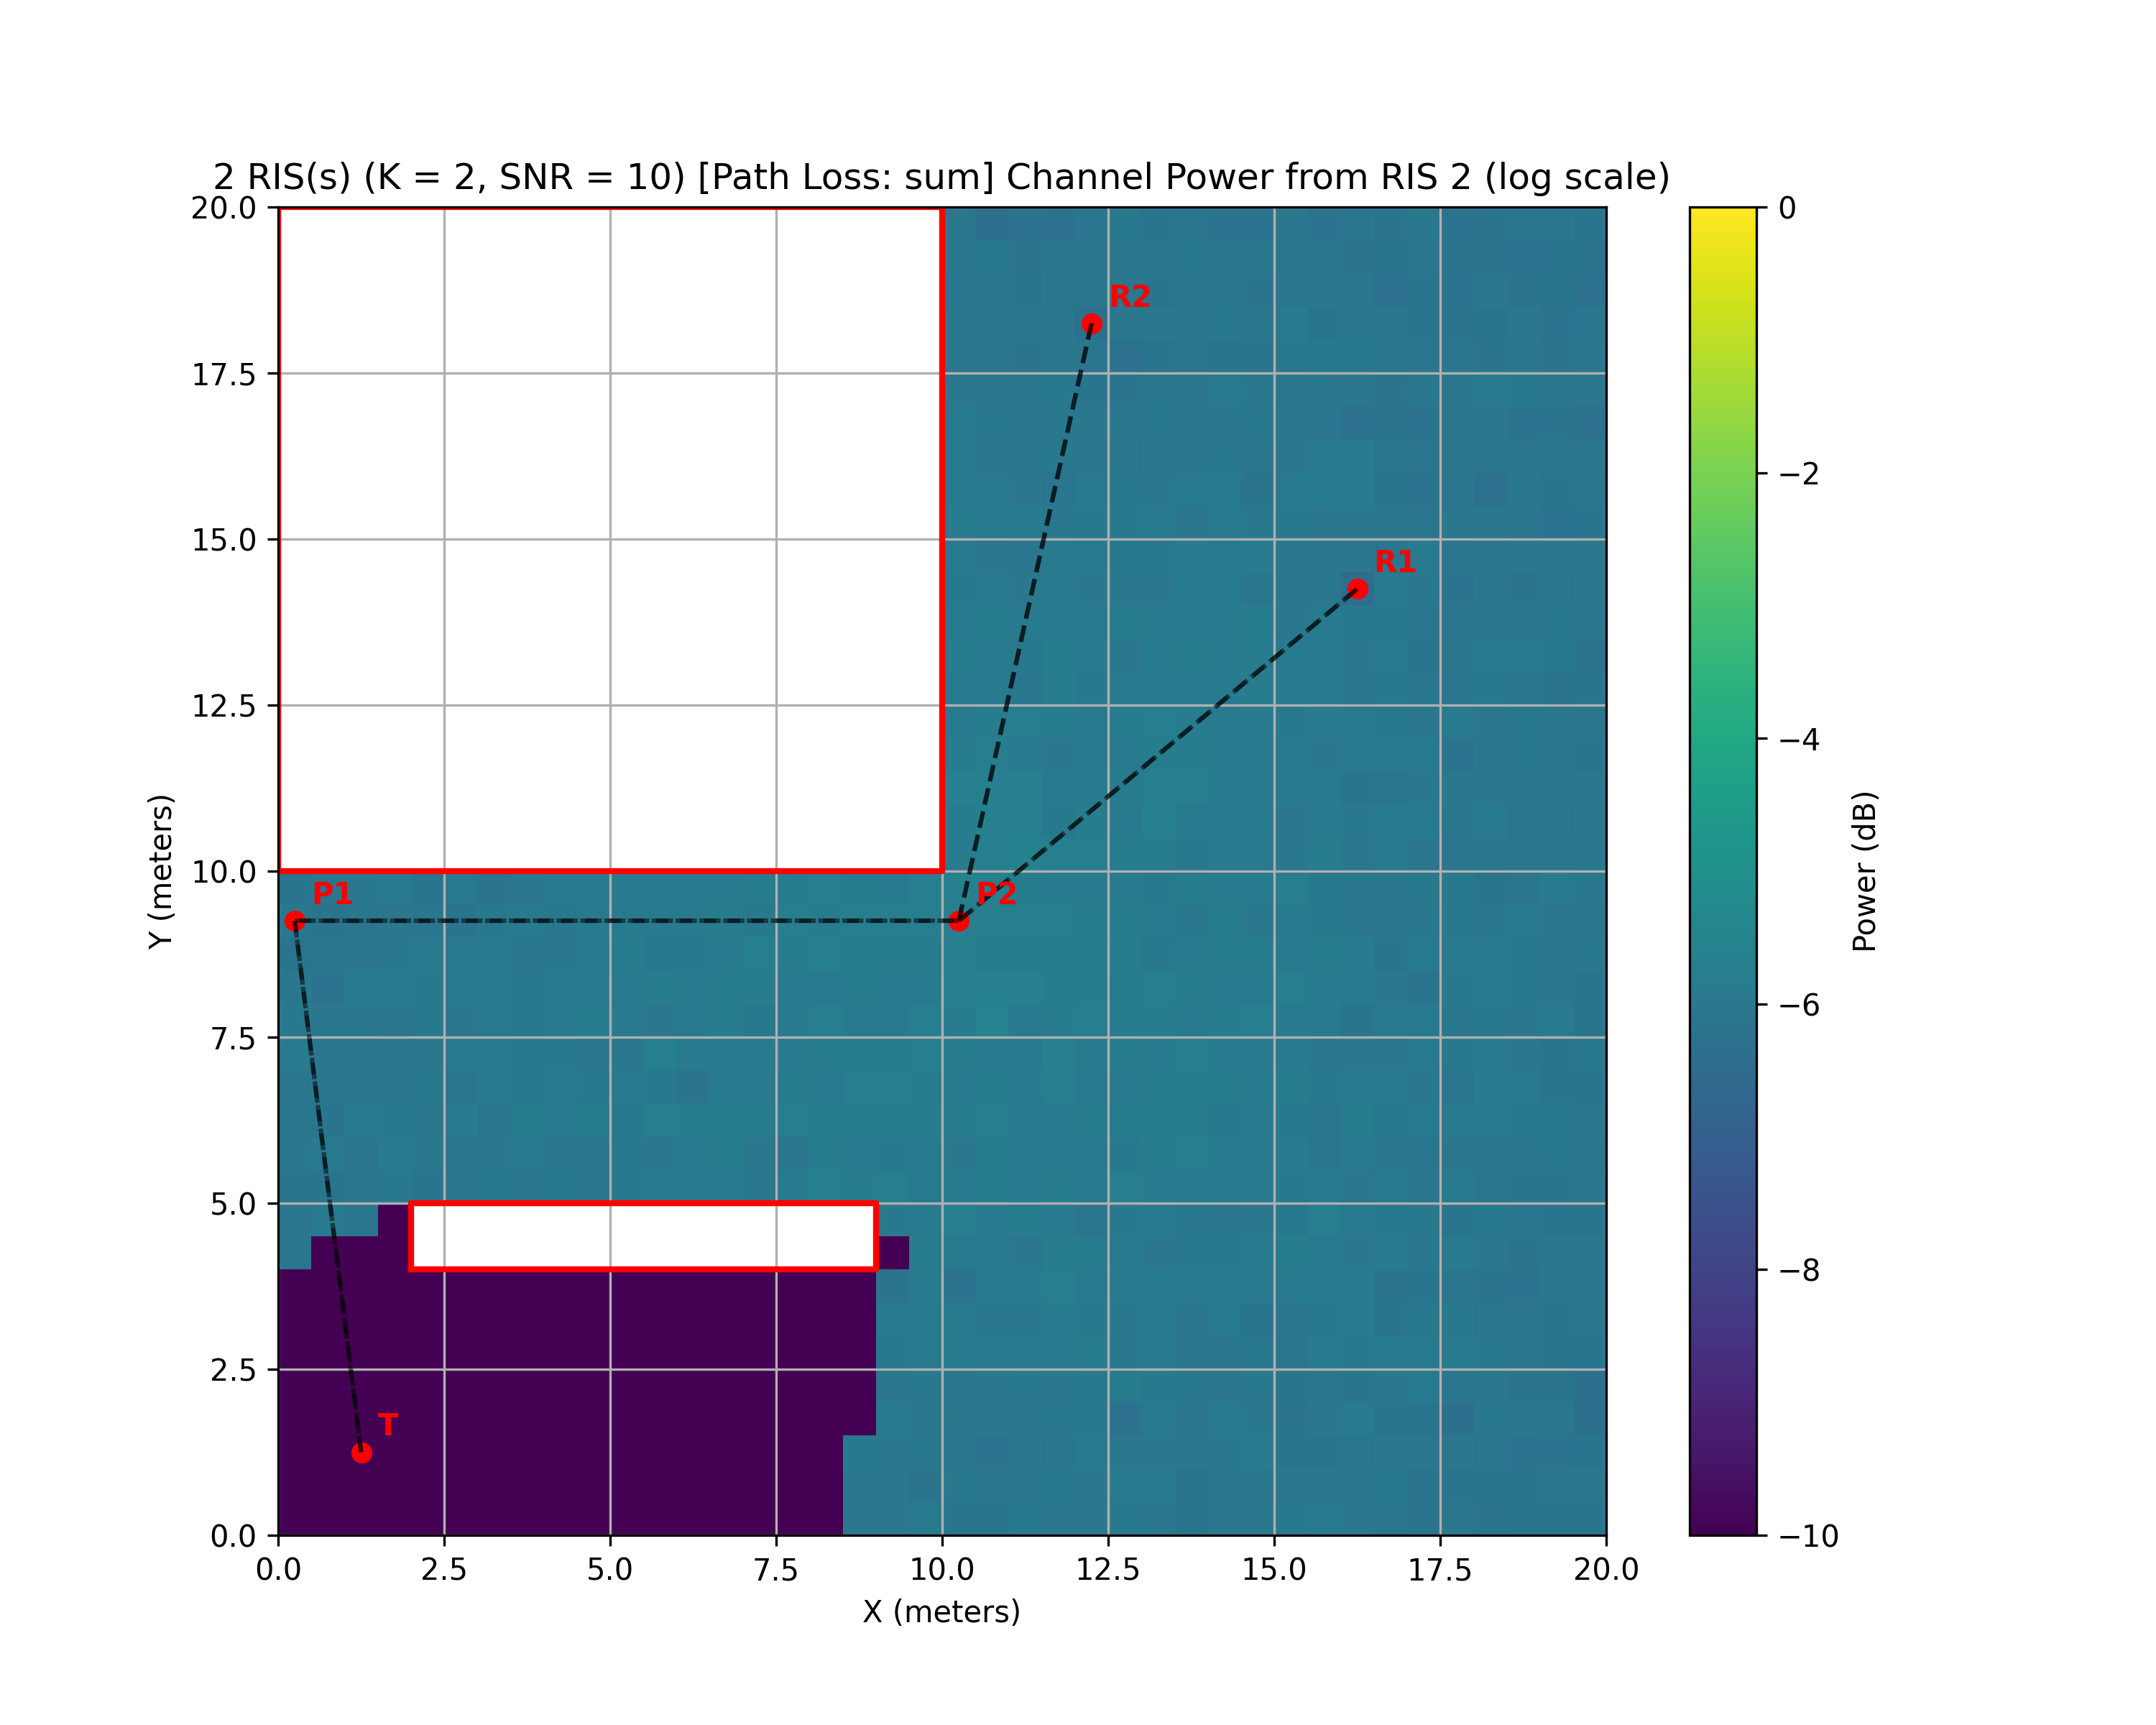
\includegraphics[width=0.8\linewidth]{imgs/heatmap-simulations/2 RIS(s) (K = 2, SNR = 10) [Path Loss_ sum] Channel Power from RIS 2 (log scale).png}
%   \caption{2 RIS(s) (K = 2, SNR = 10) [Path Loss: sum] Channel Power from RIS 2 (log scale)}
% \end{figure}

% \begin{figure}[H]
%   \centering
%   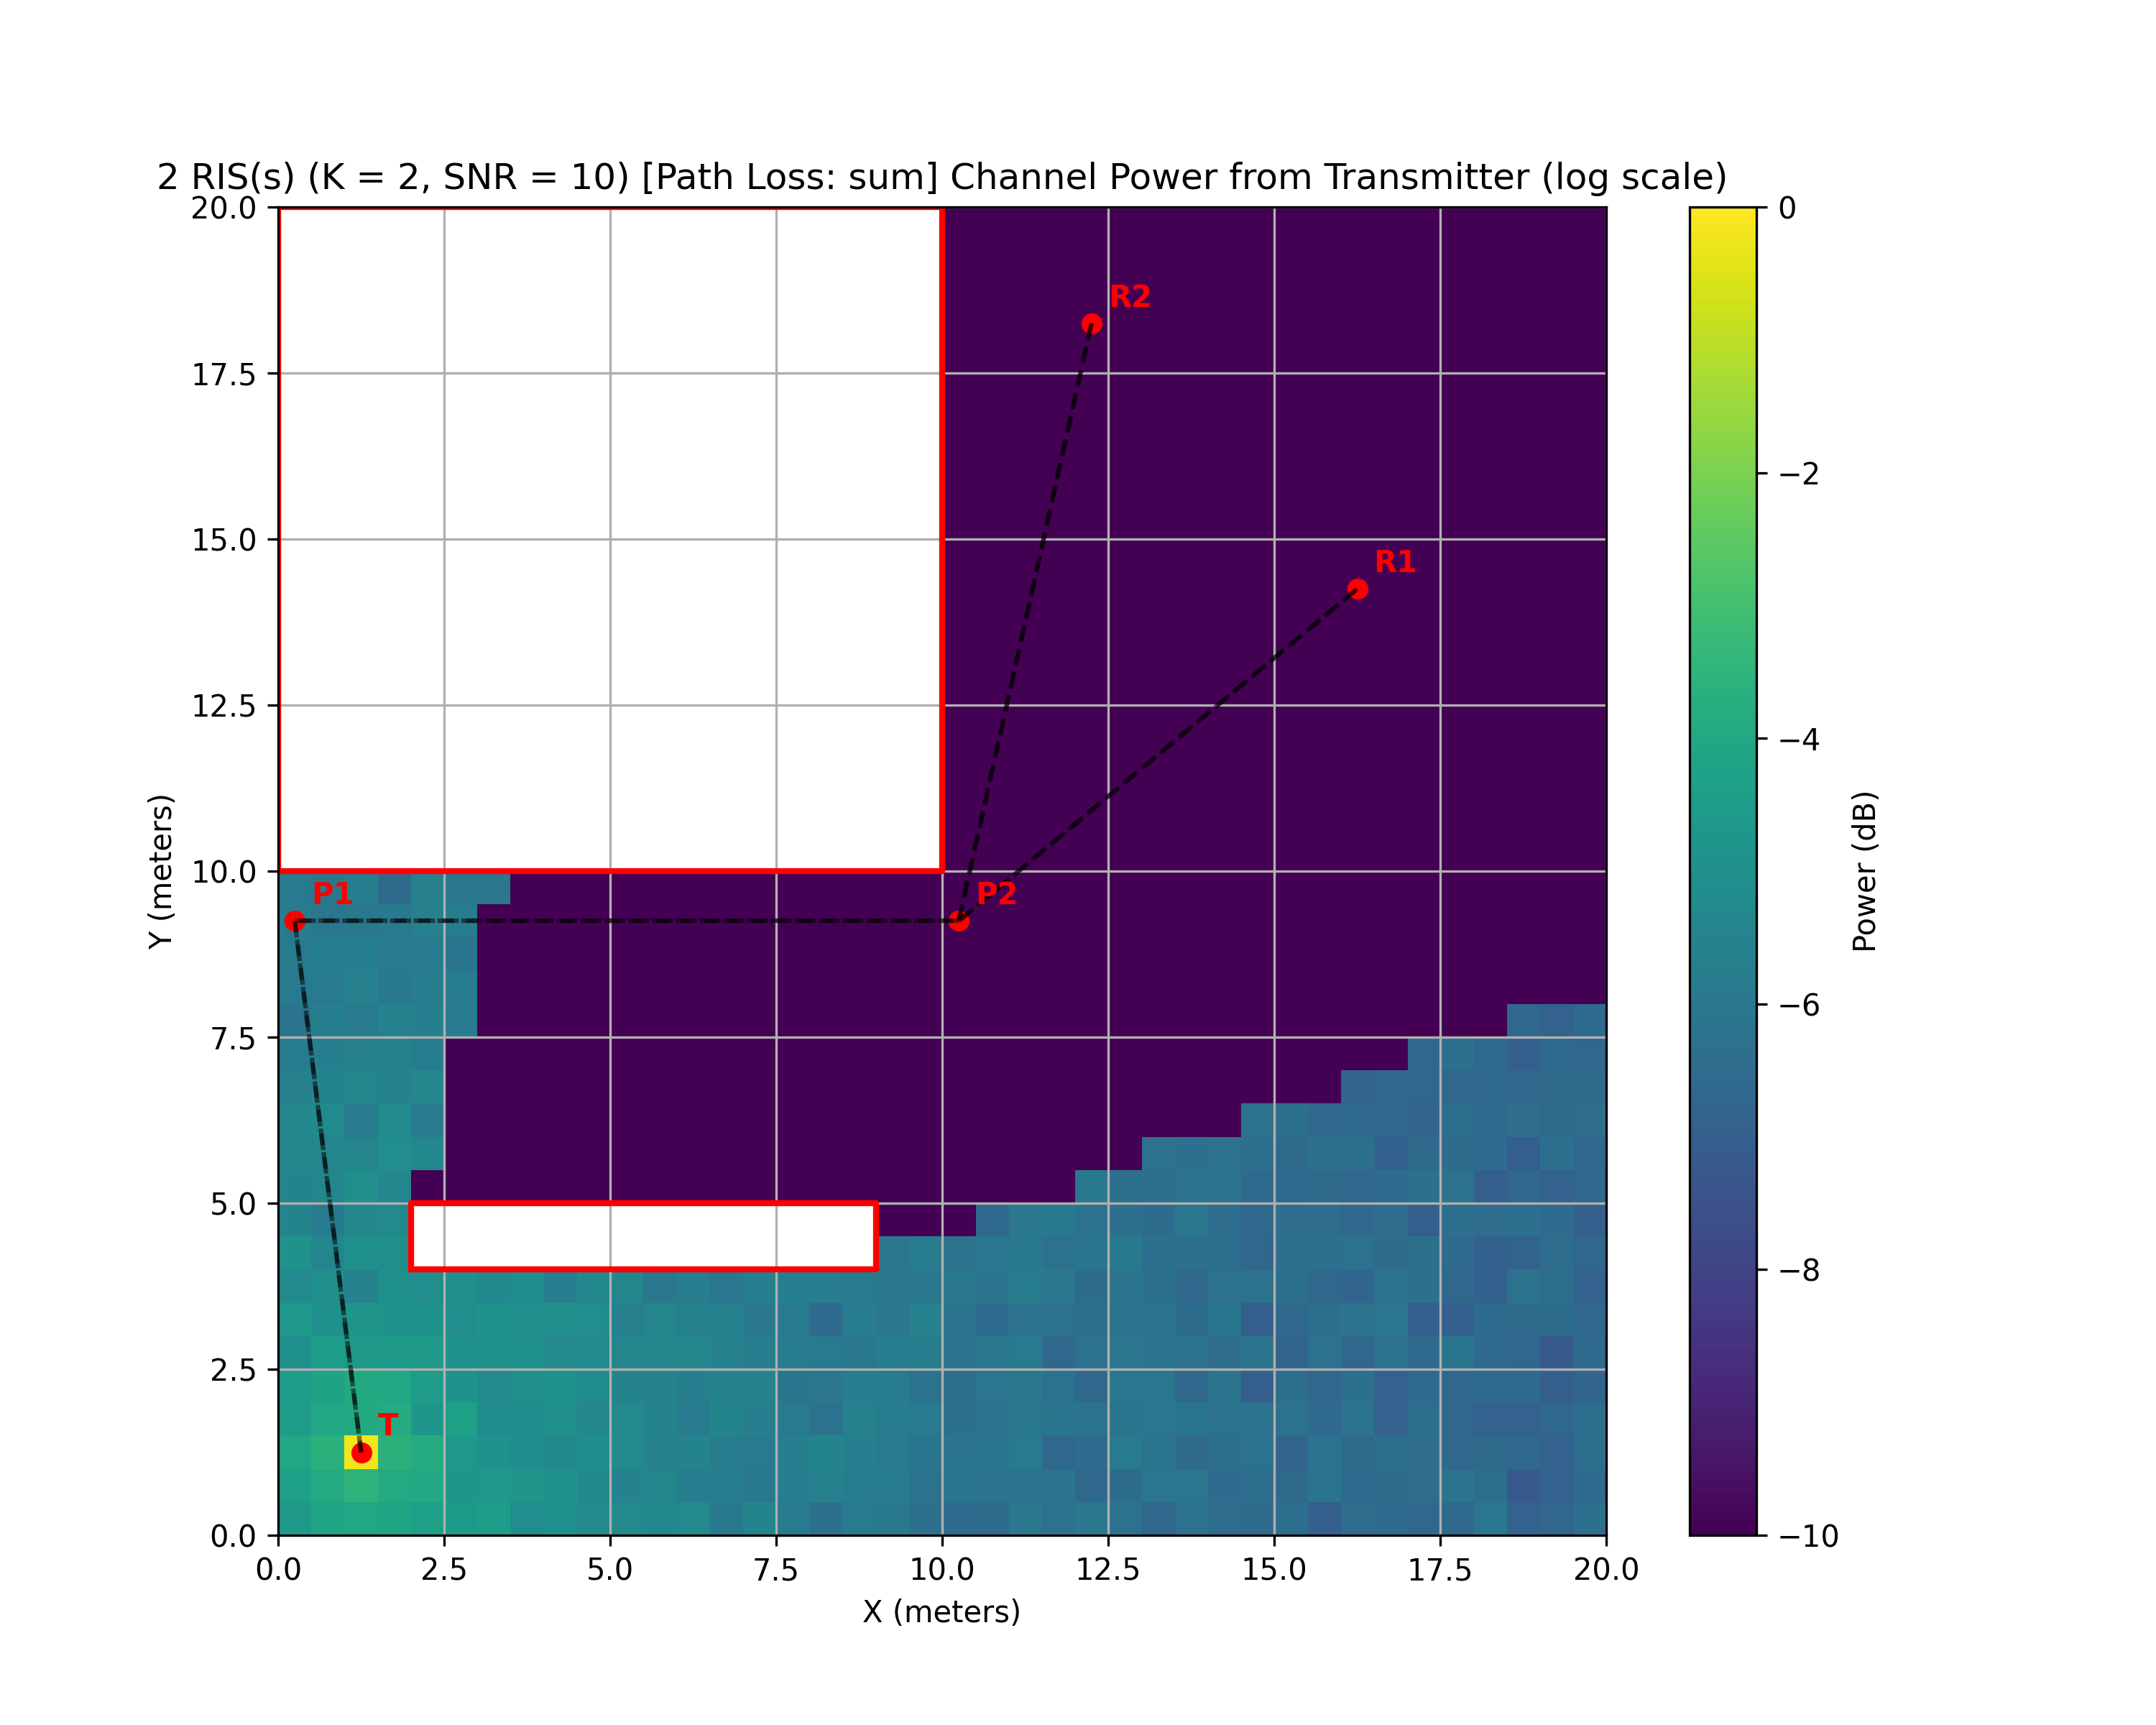
\includegraphics[width=0.8\linewidth]{imgs/heatmap-simulations/2 RIS(s) (K = 2, SNR = 10) [Path Loss_ sum] Channel Power from Transmitter (log scale).png}
%   \caption{2 RIS(s) (K = 2, SNR = 10) [Path Loss: sum] Channel Power from Transmitter (log scale)}
% \end{figure}

